\chapter{The Experimental Apparatus}
\section{The Large Hadron Collider}
The Large Hadron Collider (LHC) is a particle accelerator designed to explore the physics of particles at the energy scale of electroweak symmetry breaking. The accelerator occupies a 26.7 km tunnel beneath the Switzerland-France border near Geneva, which previously housed the Large Electron Positron Collider (LEP). Protons are accelerated in two counter-rotating beams up to a design momentum of $7~\mbox{TeV}/c$. The beams collide at four interaction points (IPs), shown in figure~\ref{fig:LHC-IPs}, where four collider detectors, ATLAS, CMS, LHCb, and ALICE, analyze the remnants of the collisions.

\begin{figure}[htbp]
	\centering
	\resizebox{0.5\textwidth}{!}{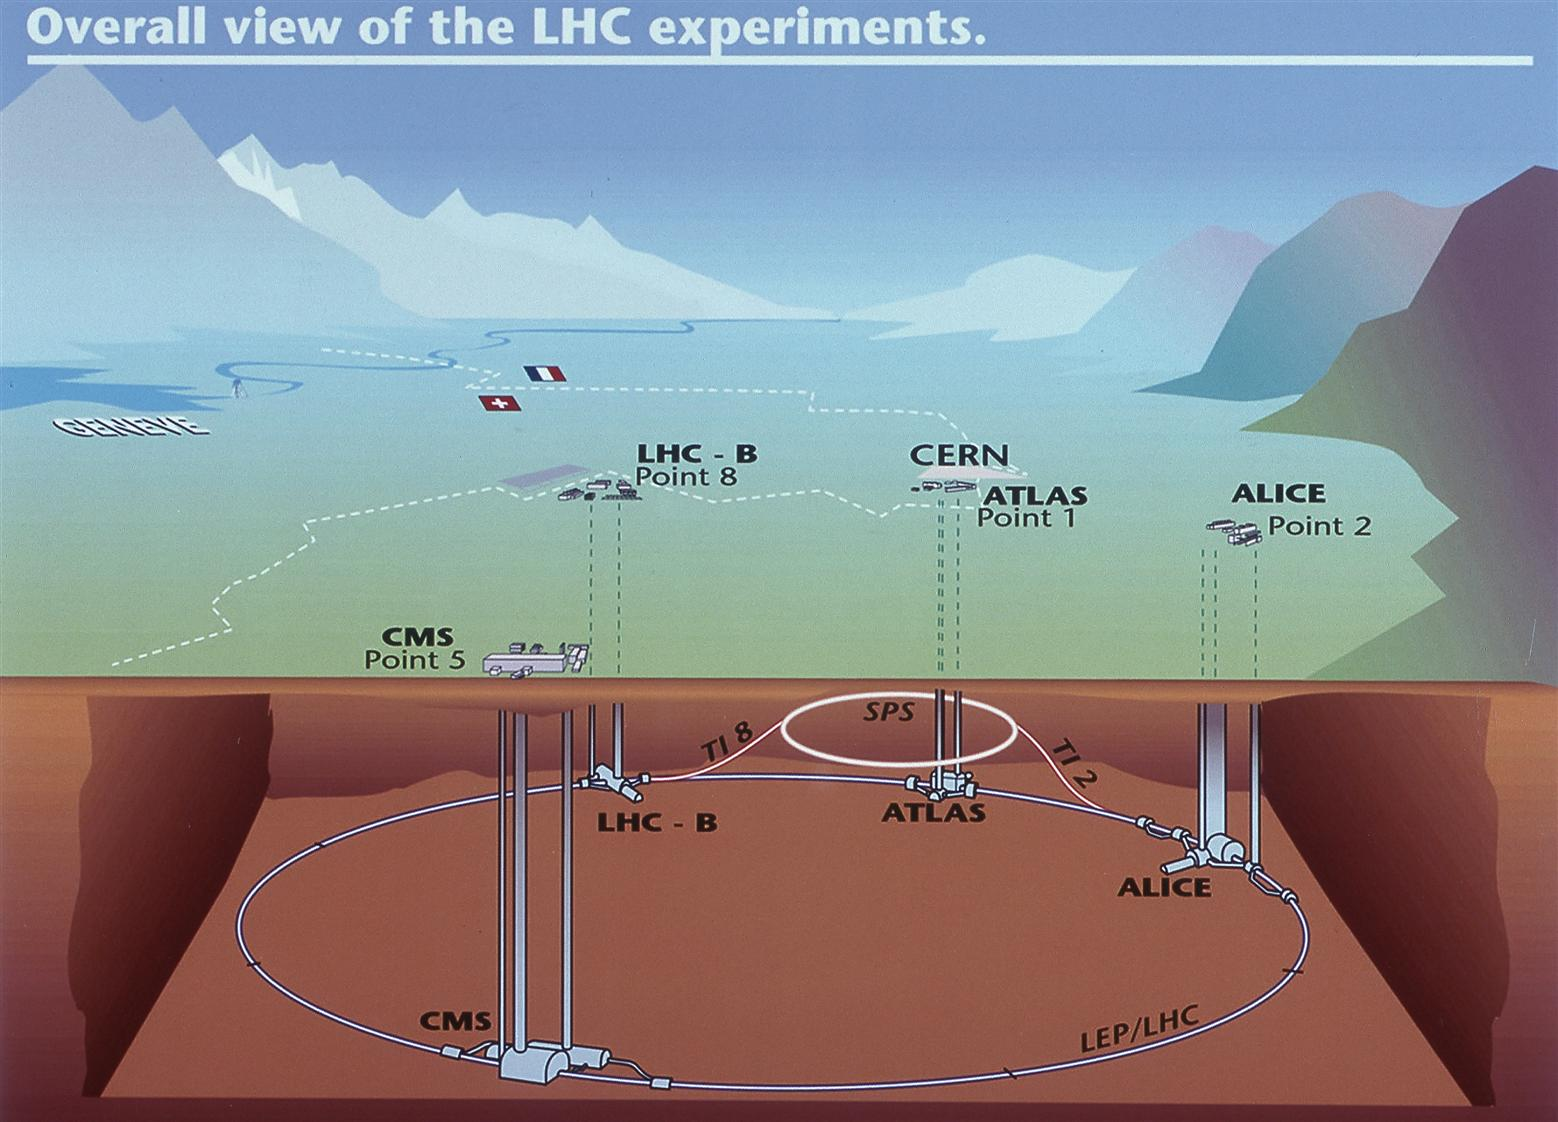
\includegraphics{figures/experiment/LHC_IPs}}
	\caption{The LHC and the four interaction points where the beams are brought into collision. The ATLAS experiment is located at interaction point 1.}
	\label{fig:LHC-IPs}
\end{figure}


The LHC project was approved in 1994 by the CERN Council, and construction proceeded over the ensuing 14 years. The collider detectors were constructed in parallel, beginning with the excavation of two additional caverns at IP1 and IP5 for the ATLAS and CMS detectors (LHCb and ALICE occupied the existing caverns at IP2 and IP8, which previously housed the DELPHI and L3 LEP experiments). The first beam was circulated on 10 September 2008; however, on 19 September, the LHC sustained severe damage due to an incident stemming from a faulty joint between magnets\footnote{A postmortem analysis implicated a bad splice between the superconducting cables of adjacent magnets as the source of the incident, with a resistance about $10^3$ times above specification. The joint melted, and 275~MJ of energy in the magnets dissipated in electric arcs, which vaporized beam pipes and breached the cryogenic vessel containing the magnets. A large amount of liquid helium entered the vacuum vessel and heated rapidly, breaking several vacuum barriers of the cryostats with a force of up to 56 tons. Ultimately, 30 dipoles and 7 quadrupoles were damaged beyond repair, and another 9 dipoles and 7 quadrupoles required repairs; 9 magnet interconnections were destroyed; 26 magnets were pushed down the tunnel; 276~MJ of energy were dissipated in electrical faults and arcs; 6 tons of helium were lost; and 2.8~km of both beam pipes were contaminated with fragments of insulation, with 1~km also contaminated with soot from molten copper and insulation.~\cite{Rossi:2010el}}. Repairs took an extra year, and the energy of the beams was reduced to $3.5-4~\mbox{TeV}$ for the first data-taking run, to mitigate the risk of another possible faulty joint. 

Proton-proton collisions at a center-of-mass energy of $\sqrt{s}=7~\mbox{TeV}$ commenced in early 2010. The LHC delivered an integrated luminosity of $\int \mathcal{L}\, dt=48.1~\mbox{pb}^{-1}$ to the ATLAS detector in 2010, and $\int \mathcal{L}\, dt=5.46~\mbox{fb}^{-1}$ in 2011. In 2012, the collision energy was increased to $\sqrt{s}=8~\mbox{TeV}$, and a dataset of $\int \mathcal{L}\, dt=22.8~\mbox{fb}^{-1}$ was delivered. 

\subsection{Accelerator Components}
The primary devices used for acceleration are synchrotrons, circular accelerators comprised of magnets and radio frequency (RF) cavities. The magnets are used to manipulate the particle beams: dipole magnets bend the beams in a circle and steer the beams down transfer lines between the accelerators, while quadrupole and higher moment magnets focus the beams. RF cavities are metallic structures used for particle acceleration. The RF cavities are driven by klystrons, radio frequency amplifiers that act as power sources, at their resonant frequency, creating an oscillating electric field inside the structure. The frequency of the RF cavities is matched to the rotation frequency of the particle beams.

The RF oscillations cause the particle beam to bunch longitudinally into so-called RF buckets, shown schematically in figure~\ref{fig:RF-bucket}. The center of the bucket corresponds to particles with the reference energy, determined by the magnets, which arrive in phase with the RF oscillations so that they experience no force. During \emph{flat-top} operation, where the particle are held at fixed energy in the synchrotron, particles at the center of the RF bucket remain stationary at that point (neglecting energy losses due to synchrotron radiation), while nearby particles oscillate around the fixed point. During a \emph{ramp}, where particles are accelerated, the magnetic fields of the dipoles are slowly increased, shifting the RF bucket and causing the particle bunches to fall on the accelerating edge of the electric field oscillations. 

\begin{figure}[htbp]
	\centering
	\resizebox{0.5\textwidth}{!}{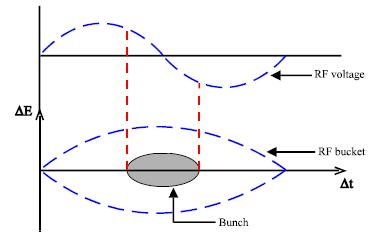
\includegraphics{figures/experiment/LHC_RF_buckets}}
	\caption{Schematic picture of an RF bucket.}
	\label{fig:RF-bucket}
\end{figure}

\FloatBarrier

\subsection{The Accelerator Complex}

\subsubsection{Injection Chain}

\begin{figure}[htbp]
	\centering
	\resizebox{3.5in}{!}{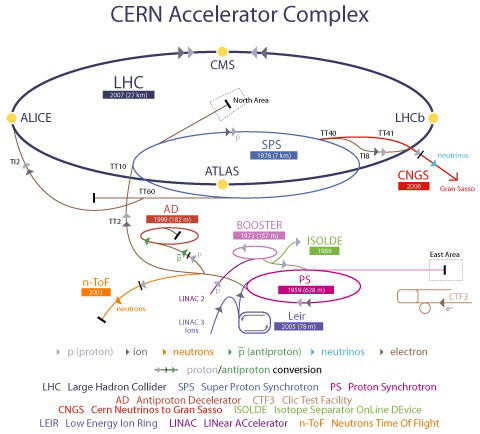
\includegraphics{figures/experiment/converted/LHC_accelerator_complex.png}}
	\caption{The LHC accelerator complex. The proton injection chain begins at LINAC2, proceeding through the booster, PS, and SPS before reaching the LHC. The facility also provides ions to the LHC, as well as a variety of particles to other experiments.}
	\label{fig:LHC-accelerator-complex}
\end{figure}


The LHC itself is the last stage of a chain of lower-energy accelerators, shown in figure~\ref{fig:LHC-accelerator-complex}. A full description of the injection chain can be found at~\cite{Benedikt:2004wm}. The staged acceleration chain preserves the high-quality of the beam over many decades of energy. It consists of a linear accelerator and three synchrotrons which were used for previous generations of experiments at CERN. The reuse of the older accelerators is economical while still meeting the stringent performance requirements of the LHC, providing up to 2808 proton bunches with a very small transverse emittance and controllable longitudinal emittance. 

Protons are produced from hydrogen gas using a duoplasmatron source, which strips electrons from protons in a high electric field. After passing through a $90~\mbox{kV}$ pre-injector, a radio frequency quadrupole (RFQ) focuses and accelerates the protons to $750~\mbox{kV}$. A linear accelerator (LINAC2) then accelerates the protons to $50~\mbox{MeV}$ using RF cavities. The protons then pass through an $80~\mbox{m}$-long transfer line into the the Proton Synchrotron Booster (PSB) and Proton Synchrotron (PS). 

The PSB consists of four stacked circular synchrotrons, $157~\mbox{m}$ in circumference, and accelerates the protons to $1.4 \GeV$. The use of four separate rings mitigates the space charge effects caused by the repulsion of protons within a bunch, which scale as $N_b/(\beta\gamma^2)$, where $N_b$ is the number of protons per bunch. The protons are then injected into single-ring PS, where the higher injection energy reduces the space charge effect. The RF cavities of the PS, operating at several frequencies, accelerate the beams to $26 \GeV$, and also split the protons into the bunches eventually inject into the LHC. Nominally, this yields 72 bunches separated by 25~ns, but for Run I, 50~ns spacing was used instead. 

The protons are extracted from the PS at intervals of 3.6~s and injected into the third synchrotron in the chain, the $7~\mbox{km}$-circumference Super Proton Synchrotron (SPS). Immediately prior to extraction, the bunches are rotated by increasing the RF voltage, reducing the longitudinal emittance in order to ease capture in the SPS RF buckets, which have a frequency of $200~\mbox{MHz}$.  Up to four PS batches are injected per SPS cycle, after which the particle are accelerated at an average of $78~\GeV/s$ to the LHC injection energy of $450 \GeV$. Flat-top is maintained for about one second, during which the injection is prepared:

\begin{itemize}
	\item The magnets used for the beam extraction are ramped, safety checks are performed, and the SPS phase is tuned to match that of the LHC.
	\item The bunch length is compressed using an RF voltage increase, as in the PS-SPS transfer.
	\item The tails of the bunches are removed, down to $3$--$3.5\sigma$.
\end{itemize}

The SPS cycle takes 21.6 seconds, leading to a total LHC filling time of about nine minutes.

\subsubsection{LHC Main Ring}
The LHC main ring accelerates protons from the injection energy of $450 \GeV$ to the collision energy, $3.5 \TeV$ or $4 \TeV$ for proton-proton collisions during Run I. The 26.7~km ring consists of eight arcs and eight straight sections, shown in figure~\ref{fig:LHC-segments}. Each straight section is called an \emph{insertion region} (IR), and contain either collider experiments or important services. IRs 1, 2, 5, and 8 contain the ATLAS, LHCb, CMS, and ALICE experiments, respectively; IR 4 contains two independent $400~\mbox{MHz}$ RF systems, one for each of the counter-rotating beams; IR 6 contains the beam dump system; and IRs 3 and 7 contain collimation systems. The beams are contained in separate beam pipes except at the collision points.

\begin{figure}[htbp]
	\centering
	\resizebox{0.5\textwidth}{!}{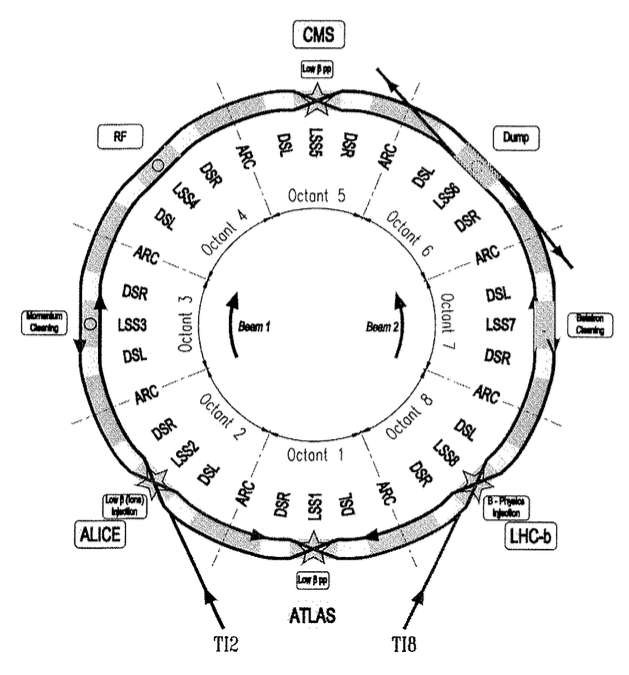
\includegraphics{figures/experiment/LHC_segments}}
	\caption{Layout of the LHC. The ring consists of eight arcs and eight long straight sections (LSS). Each junction between an arc and a LSS contains a dispersion suppressor cell (DSL, DSR). TI2 and TI8 are the two injection tunnels (``tunnel d'injection'') leading from the SPS to the LHC.}
	\label{fig:LHC-segments}
\end{figure}


The beams are controlled by over 7,000 magnets. The primary bending and focusing are performed by 1232 superconducting dipole and 392 superconducting quadrupole magnets. The dipole magnets, shown in figure~\ref{fig:LHC-dipole-magnets}, have a nominal maximum field of $8.33~\mbox{T}$ and a length of $15~\mbox{m}$. The conducting coils are constructed from Nb-Ti Rutherford cables, and are cooled to $1.9~\mbox{K}$ using superfluid helium. The dipoles have a double-bore structure, so that a single magnet provides the bending field for both beams. 

\begin{figure}[htbp]
	\centering
	\subfloat[] {
		\resizebox{0.45\textwidth}{!}{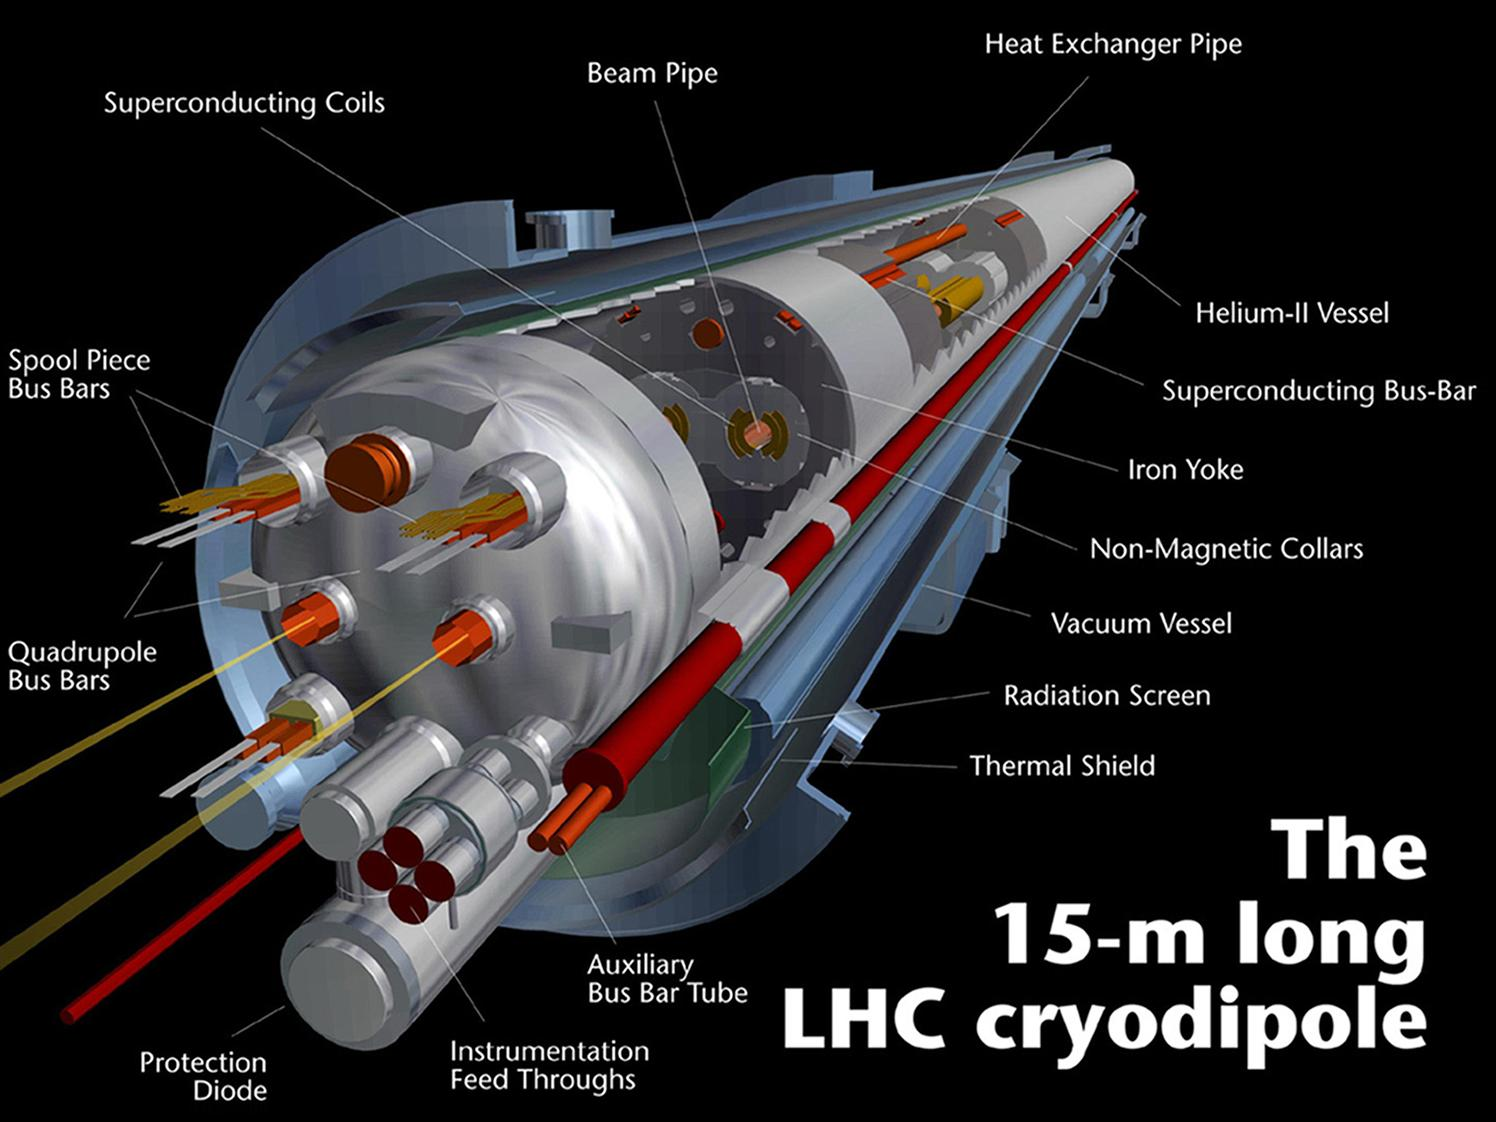
\includegraphics{figures/experiment/LHC_dipole_sketch}}
	}
	\hfill
	\subfloat[] {
		\resizebox{0.45\textwidth}{!}{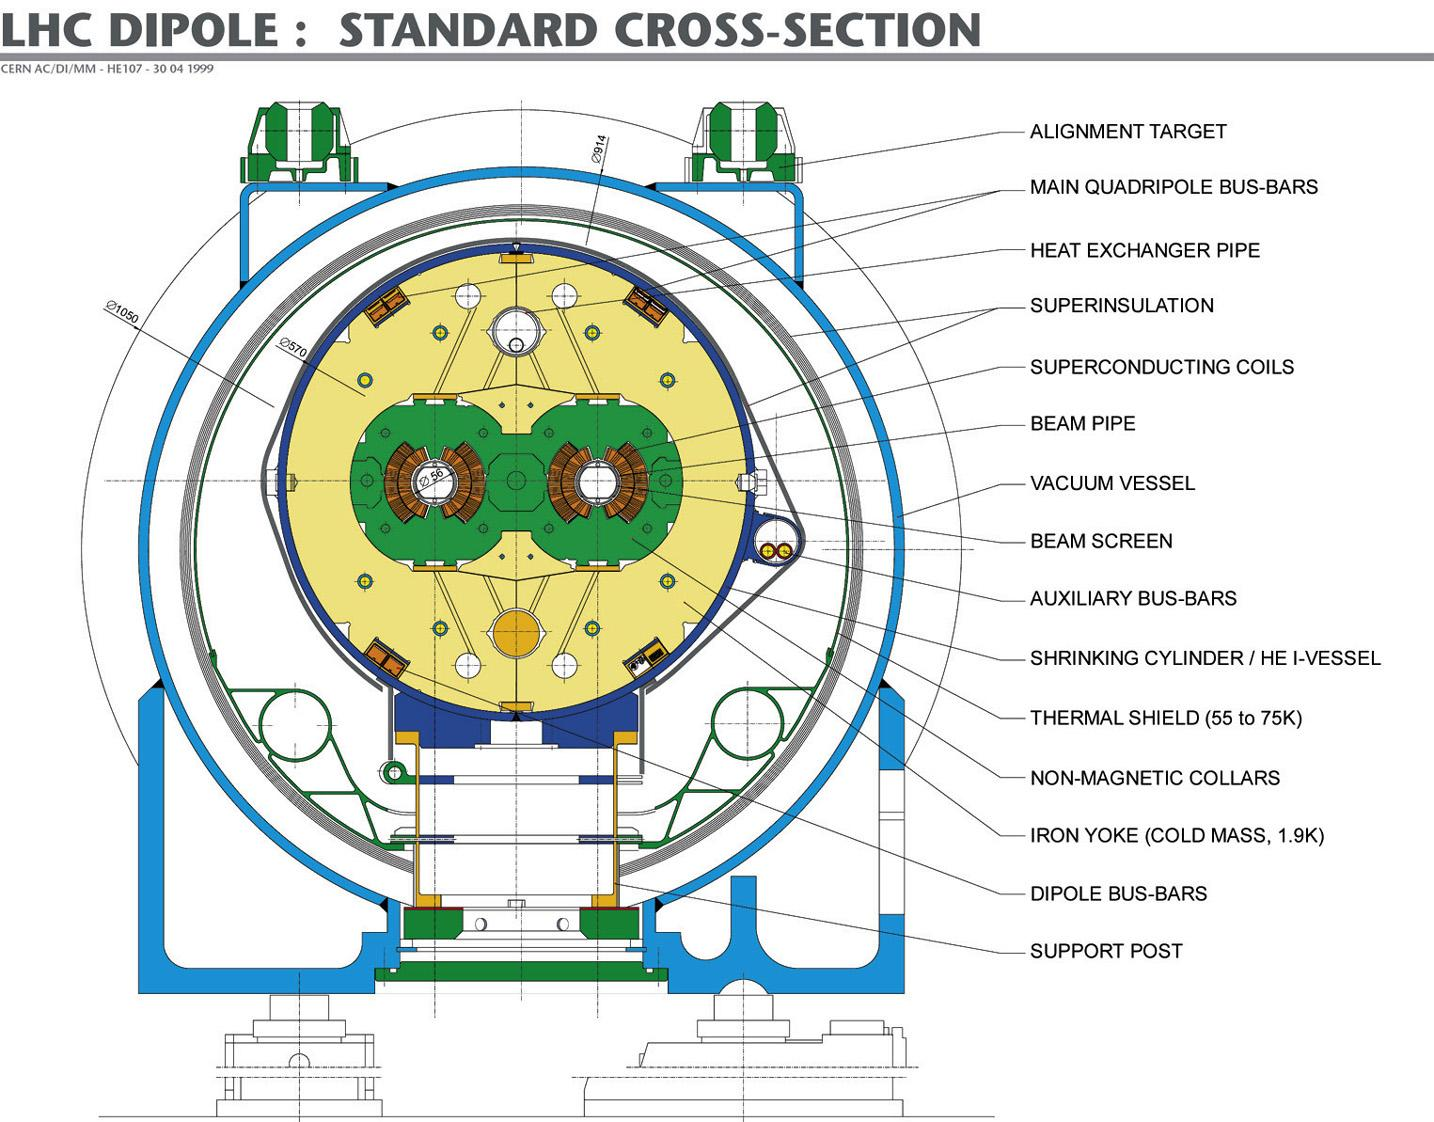
\includegraphics{figures/experiment/LHC_dipole_xsec}}
	}
	\caption{Two views of the LHC superconducting dipole magnet. The magnets are $15~\mbox{m}$ long and have two bores, one for each of the counter-rotating beams.}
	\label{fig:LHC-dipole-magnets}
\end{figure}

The acceleration is provided by two superconducting RF systems, one for each beam. The RF cavities are constructed from copper with a thin ($1-2~\micron$) layer of niobium, and operate at $4.5~\mbox{K}$. The single-cell cavities, each nominally providing $2~\mbox{MV}$, are arranged into cryomodules containing eight cells, for a total peak voltage of $16~\mbox{MV}$. A module consisting of two cells is shown in figure~\ref{fig:RF-module}. The RF frequency is $400~\mbox{MHz}$, giving an RF bucket length of $2.5~\mbox{ns}$, or $75~\mbox{cm}$. 

\begin{figure}[htbp]
	\centering
	\subfloat[ A prototype cryomodule containing two cavities.] {
		\resizebox{0.45\textwidth}{!}{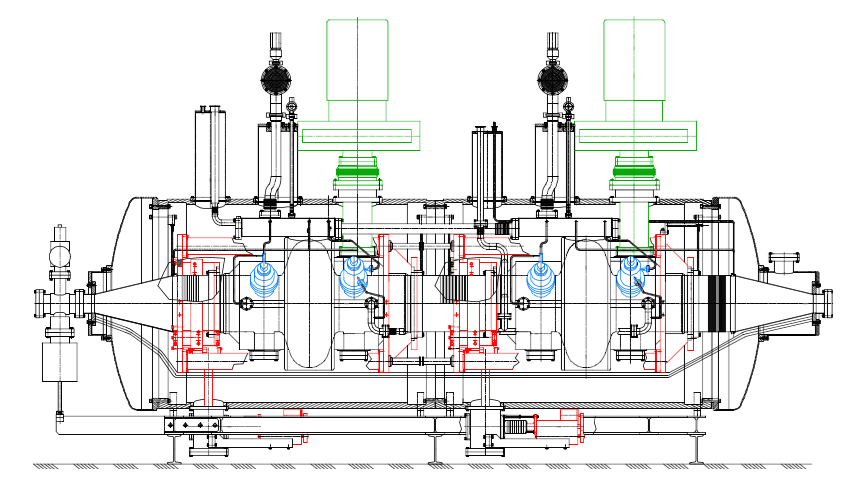
\includegraphics{figures/experiment/LHC_RF_cryomodule}}
	}
	\hfill
	\subfloat[ The RF cryomodules installed at IR4.] {
		\resizebox{0.45\textwidth}{!}{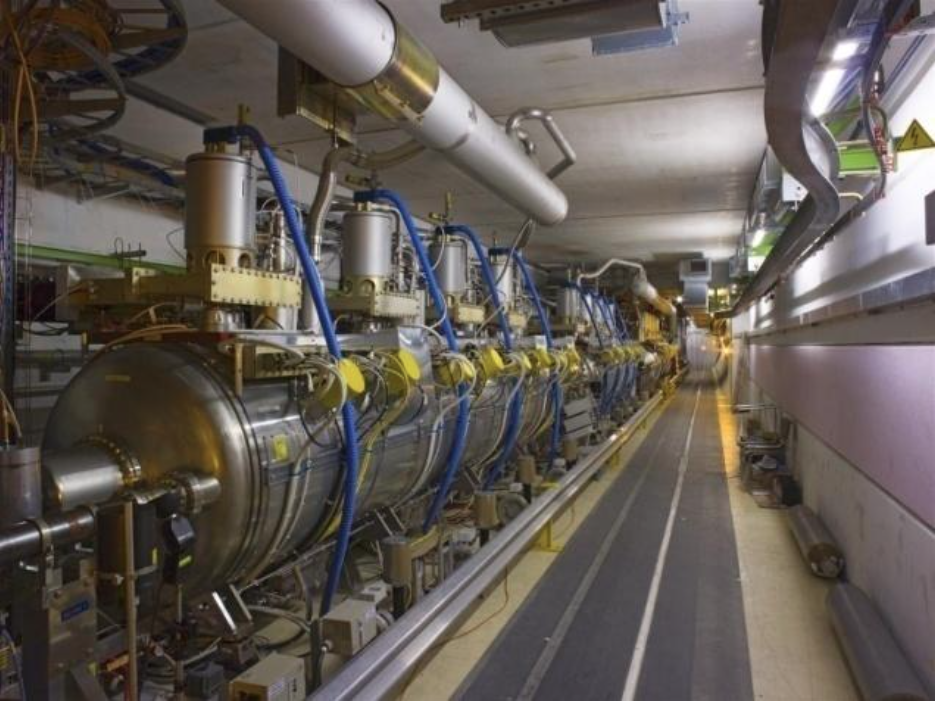
\includegraphics{figures/experiment/LHC_RF_IR4}}
	}
	\caption{The LHC RF cryomodules.}
	\label{fig:RF-module}
\end{figure}

At the collision points, the two beams converge in a single pipe for approximately $130~\mbox{m}$. A steering dipole directs the beams into collision, and a triplet of quadrupoles on each side of the interaction region focus the beam onto the interaction point, squeezing the beams in the transverse directions from a typical orbiting width of $\mathcal{O}(1~\mbox{mm})$ to a collision width of $\mathcal{O}(10~\micron)$. 


\subsection{Beam Parameters}
From the experiments' point of view, there are two main parameters to optimize in order to maximize sensitivity to new physics: the collision energy, $\sqrt{s}$, and the integrated luminosity, $L=\int \mathcal{L}\, dt$. The collision energy is limited to $\sqrt{s}=14~\mbox{TeV}$ by the bending power of the dipole magnets, which have a nominal field strength of $8.33~\mbox{T}$; however, due to the faulty splice design mentioned above, the energy was limited to $\sqrt{s}=7-8~\mbox{TeV}$ in Run I. 

The optimization of the integrated luminosity is somewhat more complicated. The instantaneous luminosity of two colliding bunches is given by:
\begin{equation}\label{eqn:lumi}
	\mathcal{L} = \frac{f_r N_1 N_2 \gamma_b}{4\pi \epsilon_n \beta_{*}} F(\alpha),
\end{equation}
where $f_r=11245.5~\mbox{Hz}$ is the LHC revolution frequency, $N_{1,2}$ are the numbers of protons in the two beams, $\gamma_b$ is the relativistic gamma factor, $\epsilon_n$ is the normalized transverse emittance, $\beta_{*}$ is the beta function at the collision point, and $F(\alpha)$ is the reduction in luminosity due to a nonzero beam crossing half-angle of $\alpha$. The total instantaneous luminosity is given by the sum of all colliding bunch pairs. 

% TO DO: beta* formula?

In general, a higher total integrated luminosity is desired. This depends on a number of factors:

\begin{itemize}
	\item The instantaneous luminosity per bunch, $\mathcal{L}=\frac{f_r N_1 N_2}{4\pi\epsilon_n \beta_{*}}$. A higher $\mathcal{L}$ increases the number of simultaneous collisions per bunch crossing (\emph{pileup}), $\mu=L_b/\sigma_{\mathrm{inel}}$, which degrades the performance of the detectors. 
	% Removed for now. According to Frank Zimmerman's slides, no beam-beam limit was found in MDs! 
	% From the accelerator's point of view, the number of protons per bunch, $N_{1,2}$, and the transverse emittance are limited by non-linear beam-beam effects~\cite{Papotti:2014vb}. Typical values during 2012 were $N_{1,2}=1.65\times 10^{11}$ and $\epsilon_n=2.5~\micron$, giving pileup values at the start of a fill of around 30, with tails up to $\sim$40. 

	\item The number of bunches in the LHC, $n_b$. During Run I, the LHC was filled with 1380 bunches with $50~\mbox{ns}$ spacing between bunches, as opposed to the nominal 2808 bunches with $25~\mbox{ns}$ spacing. The advantages of $50~\mbox{ns}$ spacing include less days needed for electron-cloud scrubbing, smalled transverse emittances, and a smaller crossing angle~\cite{Papotti:2014vb}. The primary disadvantage is a higher pileup for the experiments. 

	\item The crossing angle, $\alpha$. A nonzero crossing angle is required to prevent \emph{parasitic collisions} between bunches away from the nominal collision point. For bunches spaced by $25~\mbox{ns}$, there are 34 unwanted parasitic collision points inside the common beam pipe at each interaction region. The reduction in luminosity is:

	\begin{equation}
		F(\alpha)=\frac{1}{\sqrt{1+\left(\frac{2\alpha \sigma_z}{2\sigma^*}\right)}},
	\end{equation}
	
	where $\sigma_z$ is the RMS bunch length and $\sigma^{*}$ is the transverse beam width at the collision point. During normal 2012 running conditions, the crossing half-angle was $\alpha=145~\mu\mbox{rad}$, and the luminosity reduction factor was about $18\%$. 

	\item The fill schedule of the LHC. The instantaneous luminosity of the LHC decreases over time. The dominant loss of luminosity is due to the loss of protons from the collisions themselves, with a typical decay constant of $\tau_{\mathrm{nuclear},1/e}=29~\mbox{h}$. Including other sources of loss such as intra-bunch scattering, scattering from collisions with gas in the beam pipe, beam-beam effects, and RF noise, the typical luminosity lifetime is $\tau_L=14.9~\mbox{h}$. 

	The the fill schedule can be optimized to maximize the luminosity based on $\tau_L$ and the average turnaround time to refill the LHC after a beam dump, $T_{\mathrm{turnaround}}$. This can be quantified using the \emph{H{\"u}bner factor}, $\mathrm{HF}_{\mathrm{peak}}$, defined as the ratio of the delivered integrated luminosity to the hypothetical integrated luminosity with $\tau_L=\infty$ and $T_{\mathrm{turnaround}}=0$. In 2011, this was typically in the range $15\%$--$20\%$.
\end{itemize}

The delivered luminosity in 2011 and 2012 will be discussed later in chapter~\ref{ch:luminosity}.


\section{The ATLAS Experiment}\label{sec:the-atlas-experiment}

The ATLAS detector is a large, cylindrical collider detector located at IR1 on the LHC ring (figure~\ref{fig:LHC-IPs}). The detector measures the energy and momenta of particles produced in the collisions provided by the LHC. It consists of several subsystems occupying a cylinder with a diameter of $25~\mbox{m}$ and a length of $46~\mbox{m}$, with a combined weight of approximately 7,000 tons. Closest to the interaction region, the inner detector measures the momenta of charged particles by tracking their movement through a solenoidal magnetic field. Outside the inner detector solenoid magnet, electromagnetic and hadronic calorimeters measure the energy of electrons, photons, and hadrons. Finally, the muon spectrometer provides additional tracking and particle identification for muons in large toroidal magnetic field. 

This section describes the design of the magnets, inner detector, calorimeters, and muon spectrometer. The reconstruction of physics objects from the detector measurements is described in chapter~\ref{ch:event-reconstruction}. 

\subsection{Coordinate System}\label{sec:ATLAS-coordinate-system}

The ATLAS detector uses a right-handed coordinate system, with $\hat{x}$ pointing from the interaction point towards the center of the LHC ring, $\hat{y}$ pointing up, and $\hat{z}$ pointing along the ring towards IR2. Due to the symmetry of the detector, cylindrical coordinates ($r,\theta,\phi$) are often used, with $r$ the transverse distance from the beam line, $\theta$ the polar angle from the beamline, and $\phi$ the azimuthal angle in the $x$-$y$ plane. The polar angle can also be expressed in term of the pseudorapidity, $\eta = -\log \tan \frac{\theta}{2}$, which is useful for describing the geometry of particles in part because differences in pseudorapidity, $\Delta\eta$, are invariant under longitudinal Lorentz boosts along $\hat{z}$. For massless particles, the pseudorapidity is equal to the rapidity, $y=\frac12 \log \frac{E+p_z}{E-p_z}$. 

\subsection{Magnets}\label{sec:ATLAS-magnets}
ATLAS relies on four powerful superconducting magnets to bend the trajectories of charged particles, allowing the tracking detectors to provide measurements of their momenta. The solenoid provides a $2~\mbox{T}$ axial magnetic field in the volume of the inner detector, while the barrel and two endcap toroids provide a toroidal magnetic field ranging from $0.5$--$1~\mbox{T}$ for the muon spectrometer. The geometry of the magnets is shown in figure~\ref{fig:ATLAS-magnets-sketch}. Key parameters for the magnet system are shown in table~\ref{table:ATLAS-magnet-parameters}.

\begin{figure}[htbp]
	\centering
	\resizebox{0.6\textwidth}{!}{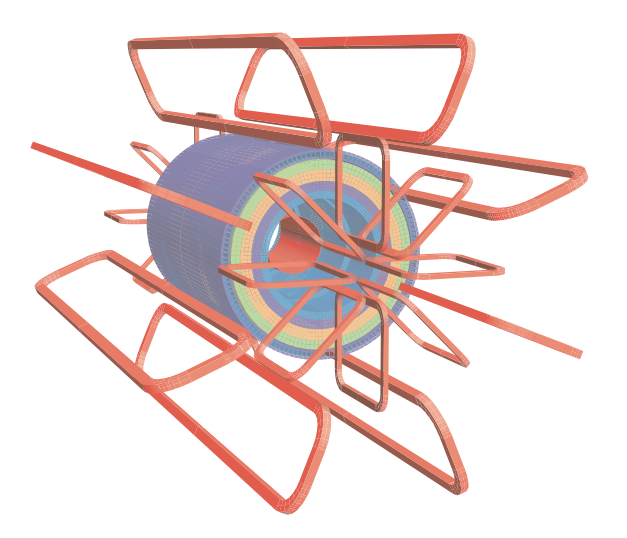
\includegraphics{figures/experiment/ATLAS_magnets_sketch}}
	\caption{The geometry of the magnet windings and tile calorimeter steel. The three toroids and solenoid are shown in red. The remaining colors show layers of the tile calorimeter with different magnetic properties and an outside return yoke.}
	\label{fig:ATLAS-magnets-sketch}
\end{figure}


\begin{table}[htbp]
	\centering
	\scriptsize
	\begin{tabular}{|l|l|c|c|c|c|}
		\hline
		\textbf{Property} & \textbf{Feature} & \textbf{Unit} & \textbf{Solenoid} & \textbf{Barrel toroid} & \textbf{End-cap toroids} \\
		\hline
		\textbf{Size} & Inner diameter & m & $2.46$ & $9.4$ & $1.65$ \\
		\hline
		 & Outer diameter & m & $2.56$ & $20.1$ & $10.7$ \\
		\hline
		 & Axial length & m & $5.8$ & $25.3$ & $5.0$ \\
		\hline
		 & Number of coils & & $1$ & $8$ & $2\times 8$ \\
		\hline
		\textbf{Mass} & Conductor & t & $3.8$ & $118$ & $2\times 20.5$ \\
		\hline
		 & Cold mass & t & $5.4$ & $370$ & $2\times 140$ \\
		\hline
		 & Total assembly & t & $5.7$ & $830$ & $2\times 239$ \\
		\hline
		\textbf{Coils} & Turns per coil & & $1154$ & $120$ & $116$ \\
		\hline
		 & Nominal current & kA & $7.73$ & $20.5$ & $20.5$ \\
		\hline
		 & Magnet stored energy & GJ & $0.04$ & $1.08$ & $2\times 0.25$ \\
		\hline
		 & Peak field in the windings & T & $2.6$ & $3.9$ & $4.1$ \\
		\hline
		 & Field range in the bore & T & $0.9$-$2.0$ & $0.2$-$2.5$ & $0.2$-$3.5$ \\
		\hline
		\textbf{Conductor} & Overall size & mm$^2$ & $30\times 4.25$ & $57\times12$ & $41\times 12$ \\
		\hline
		 & Ratio Al:Cu:NbTi & & $15.6:0.9:1$ & $28:1.3:1$ & $19:1.3:1$ \\
		\hline
		 & Number of strands (NbTi) & & $12$ & $38$-$40$ & $40$ \\
		\hline
		 & Strand diameter (NbTi) & mm & $1.22$ & $1.3$ & $1.3$ \\
		\hline
		 & Critical current (at $5~\mbox{T}$ and $4.2~\mbox{K}$) & kA & $20.4$ & $58$ & $60$ \\
		\hline
		 & Operating/critical current ratio at $4.5~\mbox{K}$ & \% & $20$ & $30$ & $30$ \\
		\hline
		 & Residual resistivity ratio (RRR) for Al & & $>500$ & $>800$ & $>800$ \\
		\hline
		 & Temperature margin & K & $2.7$ & $1.9$ & $1.9$ \\
		\hline
		 & Number of units $\times$ length & m & $4\times 2290$ & $8\times 4 \times 1730$ & $2\times8\times2\times800$ \\
		\hline
		 & Total length (produced) & km & $10$ & $56$ & $2\times13$ \\
		\hline
		\textbf{Heat load} & At $4.5~\mbox{K}$ & W & $130$ & $990$ & $330$ \\
		\hline
		 & At $60$-$80~\mbox{K}$ & kW & $0.5$ & $7.4$ & $1.7$ \\
		\hline
		 & Liquid helium mass flow & g/s & $7$ & $410$ & $280$ \\
		\hline
	\end{tabular}
	\caption{Main parameters of the ATLAS magnet system. From~\cite{TheATLASCollaboration:2008fg}.}
	\label{table:ATLAS-magnet-parameters}
\end{table}




\subsubsection{Solenoid}\label{sec:ATLAS-magnets-solenoid}

The central solenoid, shown in figure~\ref{fig:solenoid}, occupies the volume between the inner detector and the electromagnetic calorimeter, with an inner radius of $2.46~\mbox{m}$, an outer radius of $2.56~\mbox{m}$, and a length of $5.8~\mbox{m}$. The single coil has 1154 windings made of high strength Al-stabilized NbTi conductor. With a nominal current of $7.73~\mbox{kA}$, the magnetic field is $1.998~\mbox{T}$ at the center of the solenoid, falling to $1.8~\mbox{T}$ at $z=1.7~\mbox{m}$ and $0.9~\mbox{T}$ the end of the inner detector cavity.  The magnetic flux is returned via the steel in the hadronic calorimeter and its support structures. Liquid helium is used to cool the superconducting coil to an operating temperature of $4.5~\mbox{K}$. At nominal current, the stored energy is $40~\mbox{MJ}$. 

The longitudinal and radial magnetic field components are shown for different $R$ and $z$ values in figure~\ref{fig:ATLAS-solenoid-Bfield}.

\begin{figure}[htbp]
	\centering
	\resizebox{0.6\textwidth}{!}{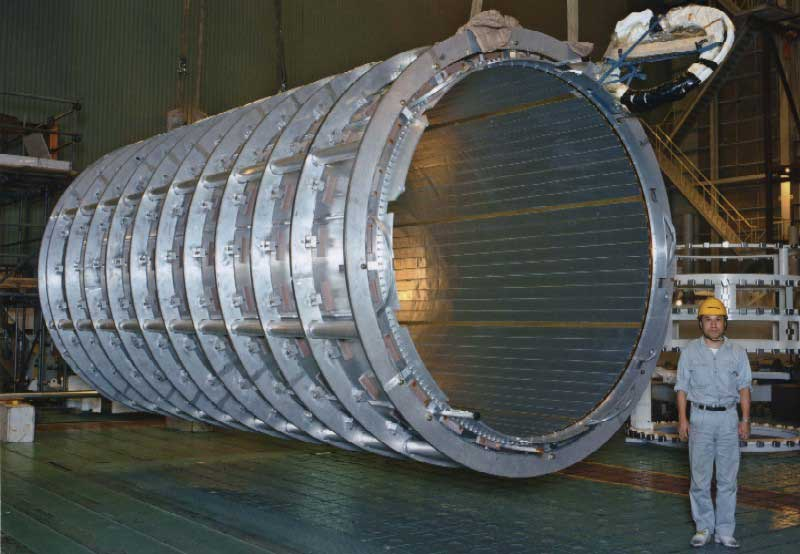
\includegraphics{figures/experiment/ATLAS_solenoid_2}}
	\caption{The central solenoid in the factory after completion of the coil winding~\cite{TheATLASCollaboration:2008fg}.}
	\label{fig:solenoid}
\end{figure}

\begin{figure}[htbp]
	\centering
	\resizebox{0.6\textwidth}{!}{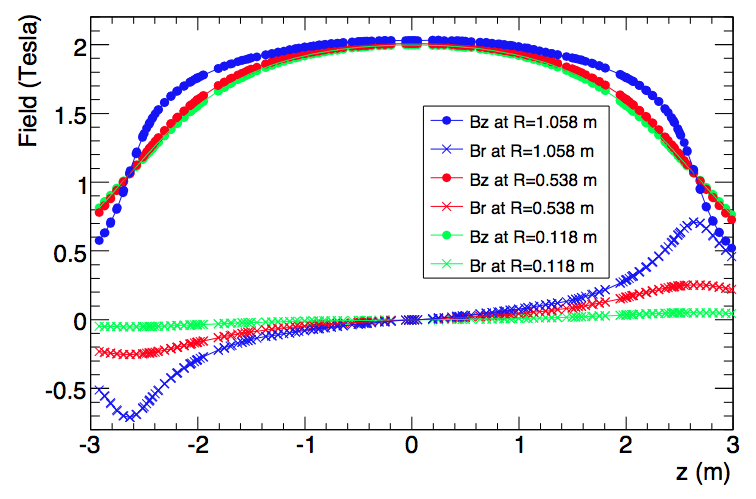
\includegraphics{figures/experiment/ATLAS_solenoid_Bfield}}
	\caption{The solenoid magnetic field in the radial ($B_r$) and longitudinal ($B_z$) directions, shown as a function of $z$ for $\phi=20\pi/16$ at different values of $R$. The field determined from a fit of the field model to measurements using an array of Hall probes~\cite{Aleksa:2008br}.}
	\label{fig:ATLAS-solenoid-Bfield}
\end{figure}



\subsubsection{Toroid}\label{sec:ATLAS-magnets-toroid}

The magnetic field for the muon spectrometer is provided by three large toroid magnets, each with eight superconducting coils. The magnets are shown in figure~\ref{fig:ATLAS-toroids}. The barrel toroid measures $25.3~\mbox{m}$ in length, with inner and outer diameters of $9.4~\mbox{m}$ and $20.1~\mbox{m}$, respectively. The two end-cap toroids are $5.0~\mbox{m}$ in length, with inner and outer diameters of $1.65~\mbox{m}$ and $10.7~\mbox{m}$, respectively. Both types of toroid contain eight coils, with 120 windings per coil in the barrel and 116 windings per coil in the end-caps. The end-cap coils are rotated by $22.5^{\circ}$ from the barrel coils to optimize the bending power in the overlap region between the magnets. Like the solenoid, the conductor is Al-stabilized NbTi, operated at $4.5~\mbox{K}$. The nominal current is $20.5~\mbox{kA}$, producing a magnetic field that varies from $0.15~\mbox{T}$ to $2.5~\mbox{T}$ in the barrel region, and $0.2~\mbox{T}$ to $3.5~\mbox{T}$ in the end-caps. The total stored energy at nominal current is $1.58~\mbox{GJ}$. 

The field integral of the toroid is shown as a function of $\eta$ in figure~\ref{fig:ATLAS-toroid-Bintegral}. The field integral drops at the boundary between the barrel and end-caps, where the fields from the two magnets partially cancel. 

\begin{figure}[htbp]
	\centering
	\subfloat[ Barrel toroid.] {
		\resizebox{0.45\textwidth}{!}{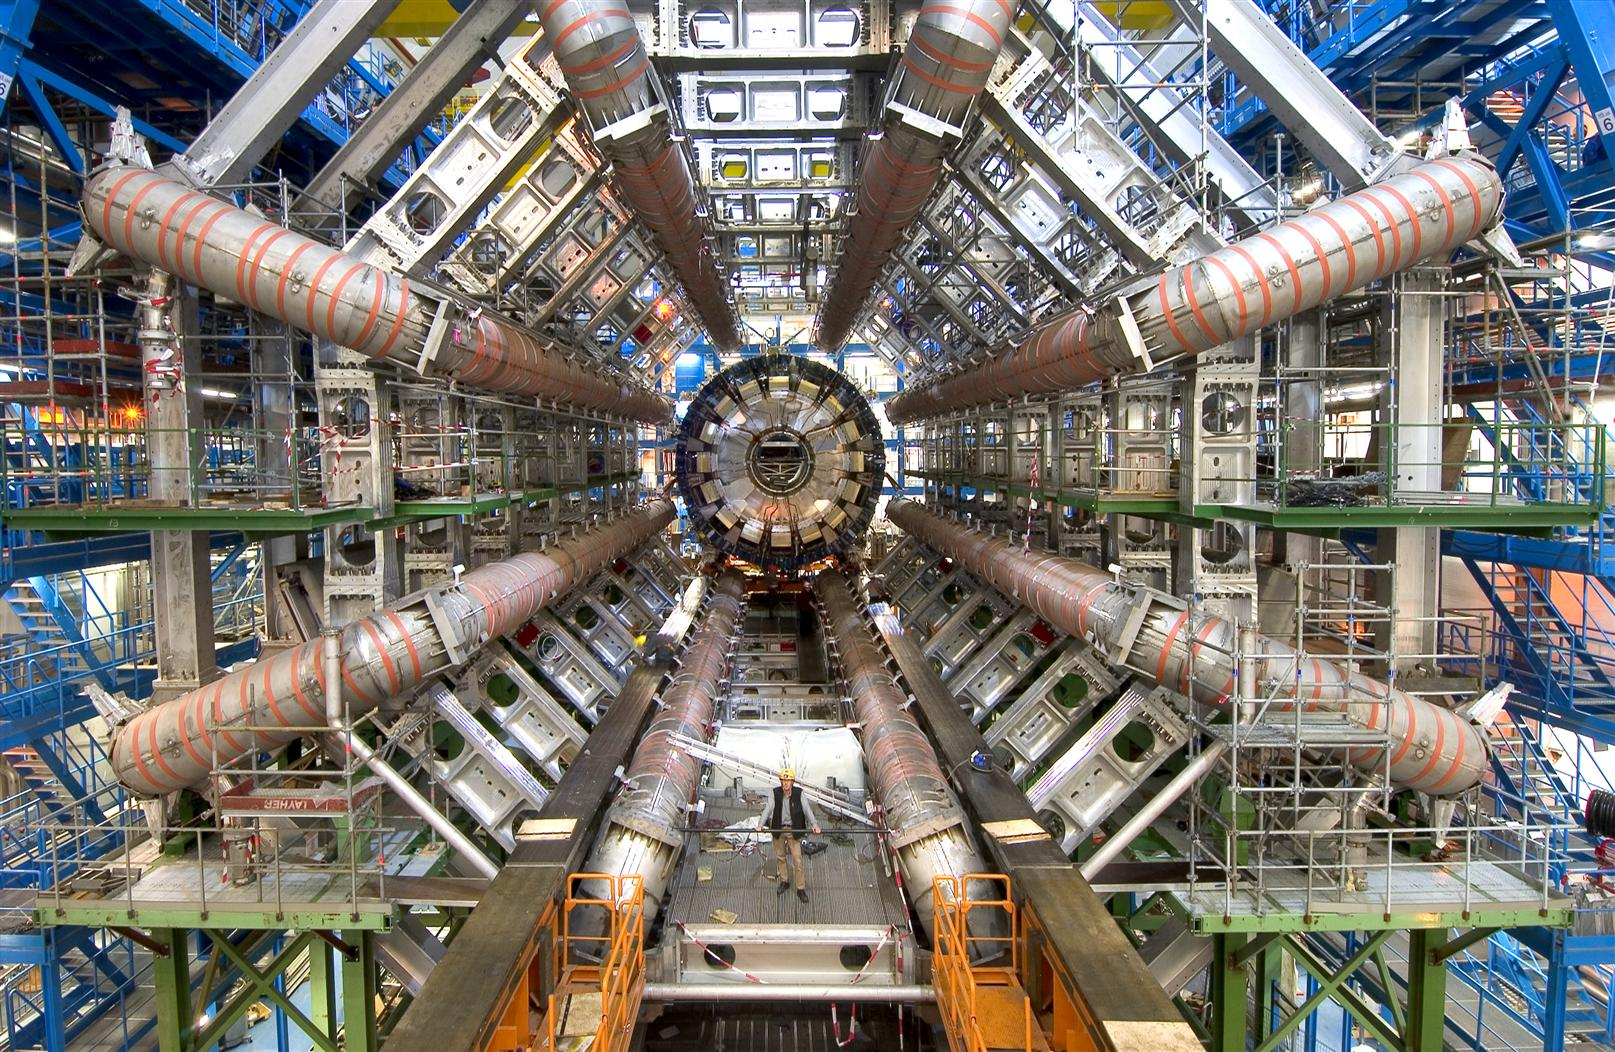
\includegraphics{figures/experiment/ATLAS_toroid}}
	}
	\hfill
	\subfloat[ End-cap toroid, inserted into the barrel toroid.] {
		\resizebox{0.45\textwidth}{!}{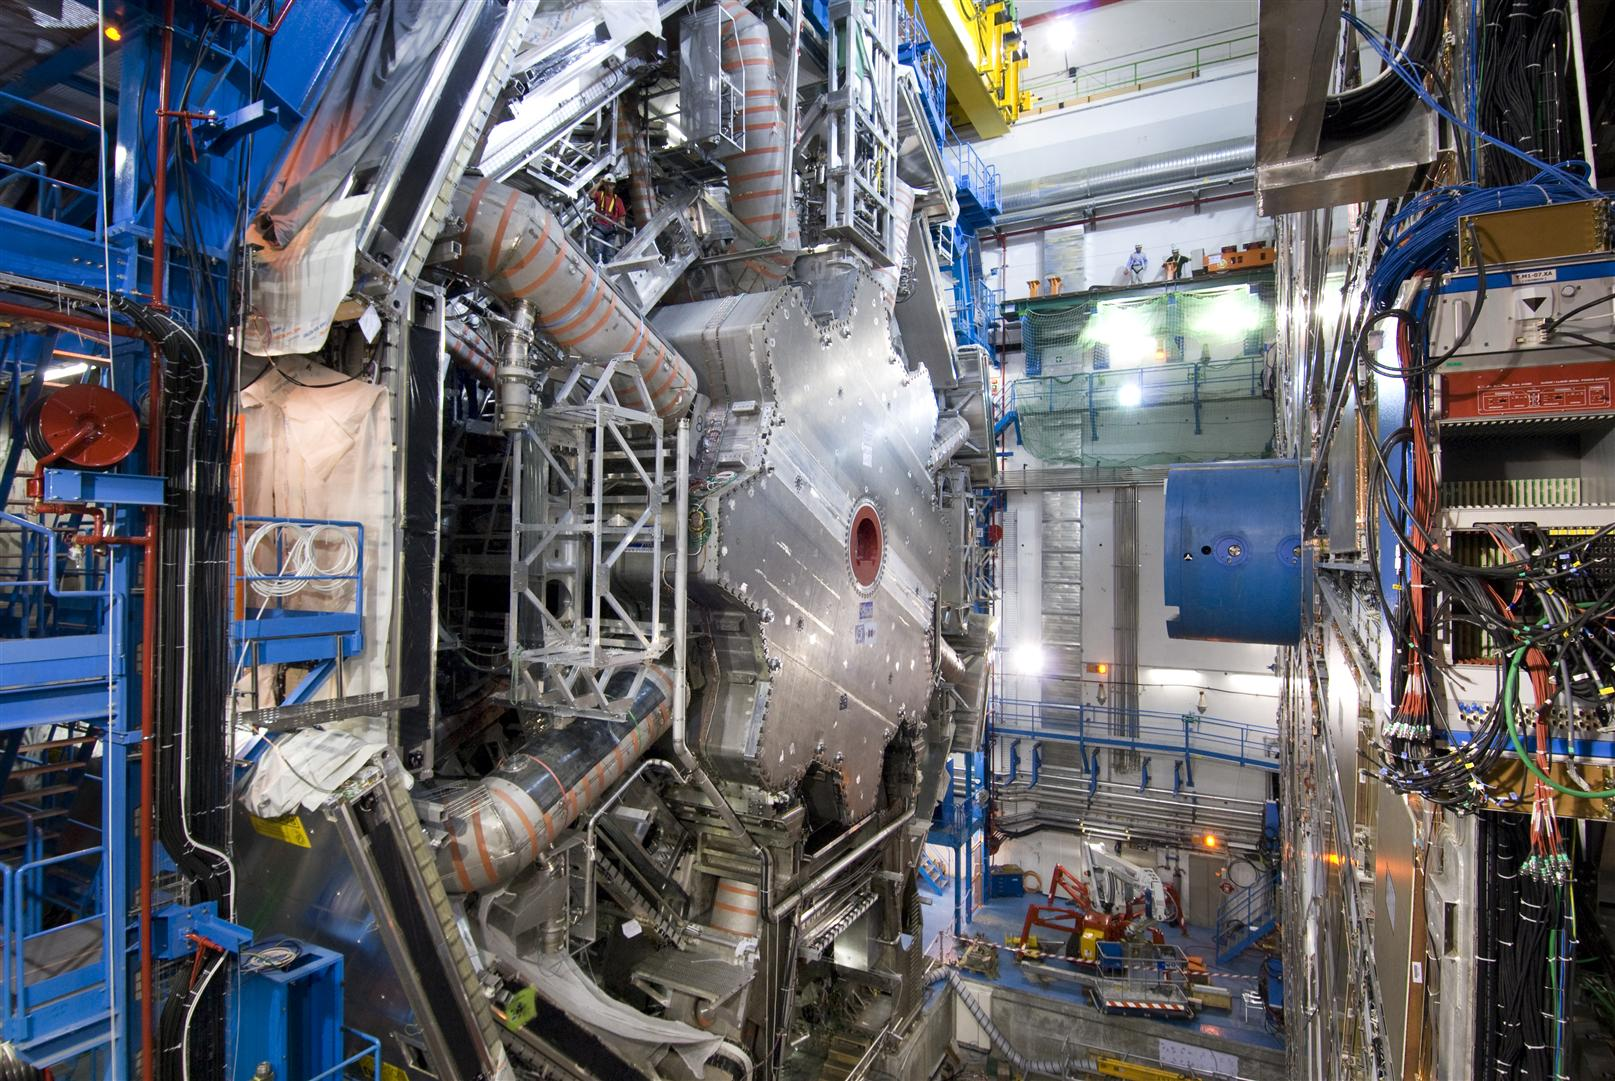
\includegraphics{figures/experiment/ATLAS_toroid_endcap_inserted2}}
	}
	\caption{Images of the barrel and end-cap toroid magnets during installation.}
	\label{fig:ATLAS-toroids}
\end{figure}

\begin{figure}[htbp]
	\centering
	\resizebox{0.6\textwidth}{!}{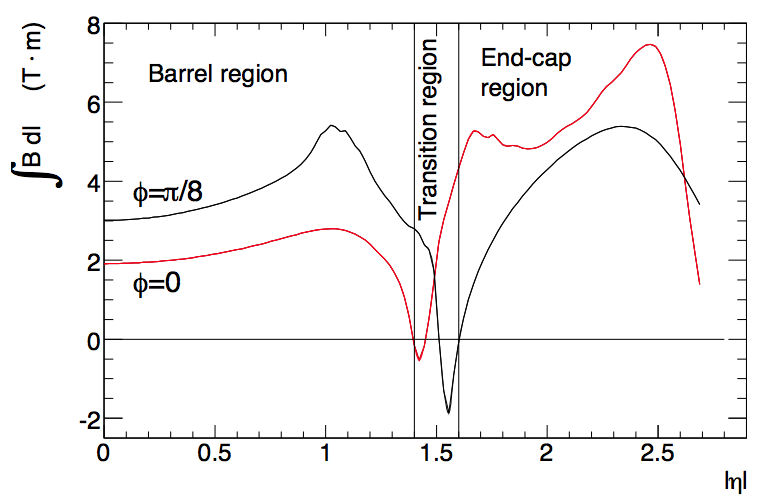
\includegraphics{figures/experiment/ATLAS_toroid_Bintegral}}
	\caption{The predicted toroid magnetic field integral as a function of $|\eta|$. The integral is taken over a straight line through the interaction point, from the innermost to the outermost muon detector (section~\ref{sec:ATLAS-muon-spectrometer}).}
	\label{fig:ATLAS-toroid-Bintegral}
\end{figure}



\subsection{Inner Detector}\label{sec:ATLAS-inner-detector}

The inner detector performs tracking of charged particles traversing the $2~\mbox{T}$ solenoidal magnetic field in the pseudorapidity range $|\eta|<2.5$. It also performs electron identification in the range $|\eta|<2.0$. It consists of three subdetectors occupying the volume closest to the interaction region, directly outside the beam pipe, as shown in figure~\ref{fig:ATLAS-ID}. Proceeding outwards from the interaction point, these are the pixel detector, the semiconductor tracker (SCT), and the transition radiation tracker (TRT). The pixel detector provides three track measurements with high spatial resolution using silicon pixels. The SCT provides an additional four measurements using silicon strips. Finally, for particles with $|\eta|<2.0$, the TRT provides an average of 36 measurements per track using gas-filled straw tubes, which aids the pattern recognition, improves the momentum resolution, and performs electron identification. Examples of trajectories of $10 \GeV$ particles through the barrel and end-cap layers are shown in figure~\ref{fig:ATLAS-ID-tracks}.

\begin{figure}[htbp]
	\centering
	\subfloat[ 3D model of the inner detector, showing the arrangement of the pixel detector, SCT, and TRT in the barrel and end-caps.] {
		\resizebox{0.45\textwidth}{!}{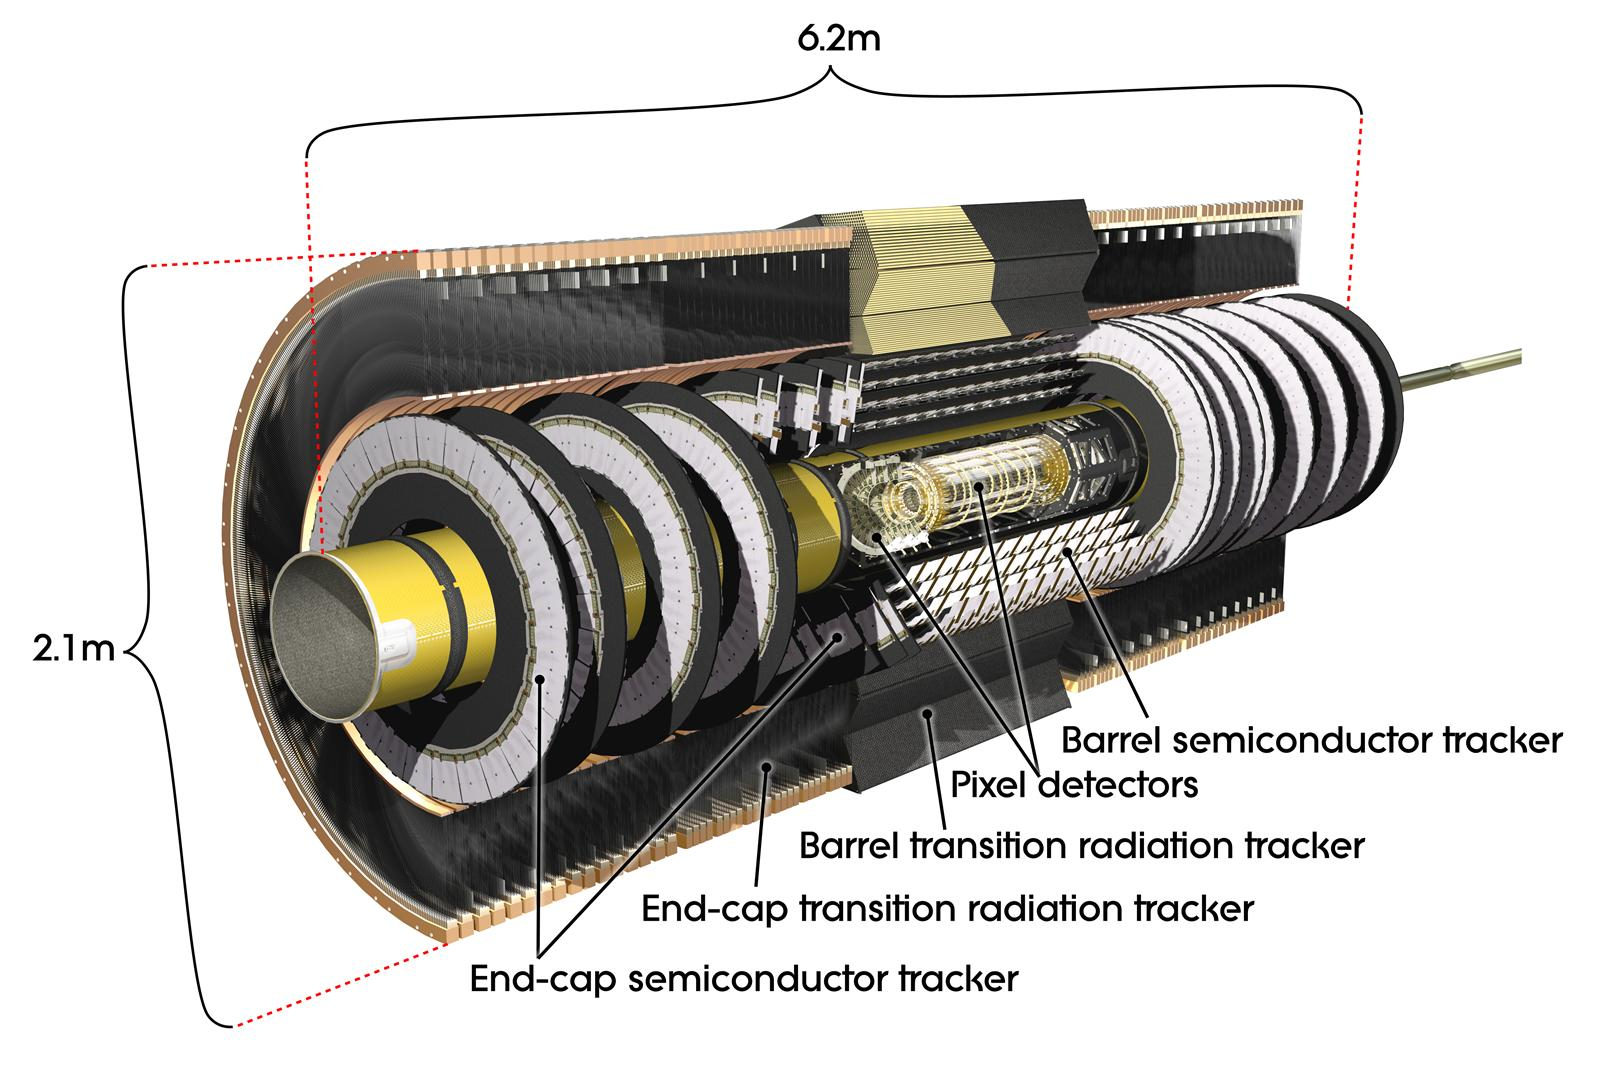
\includegraphics{figures/experiment/ATLAS_ID_sketch}}
	}
	\hfill
	\subfloat[ Layout of the inner detector in the $R-z$ plane.] {
		\resizebox{0.45\textwidth}{!}{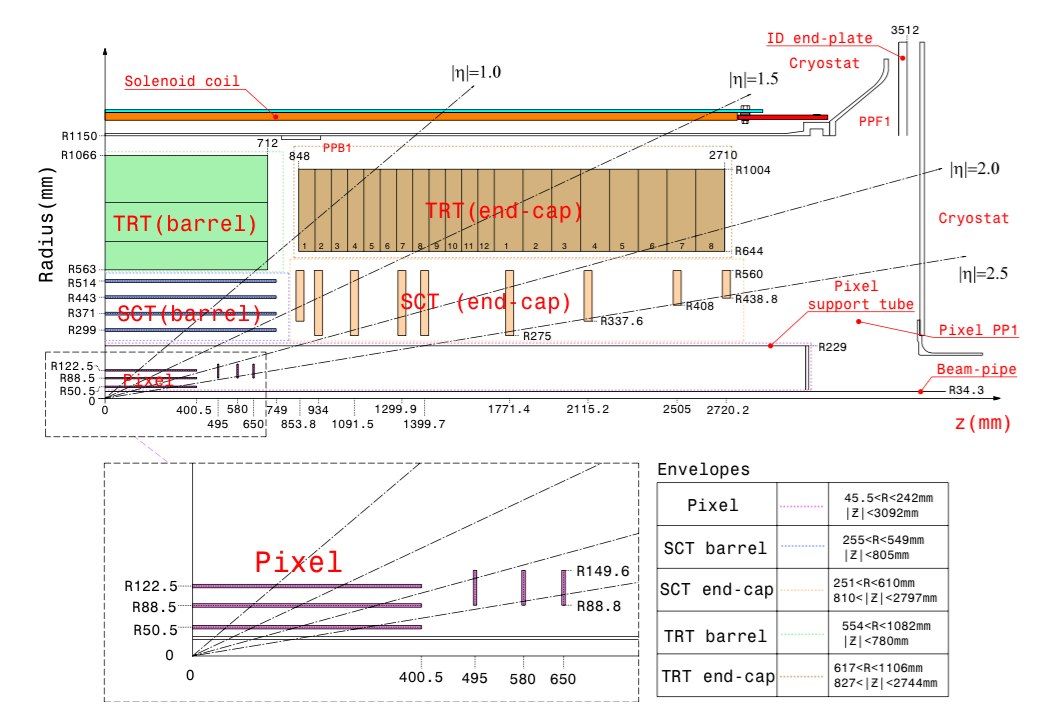
\includegraphics{figures/experiment/ATLAS_ID_layout_rz}}
	}
	\caption{Layout of the ATLAS inner detector.}
	\label{fig:ATLAS-ID}
\end{figure}

\begin{figure}[htbp]
	\centering
	\subfloat[ Trajectory of a $10 \GeV$ charged particle with $\eta=0.3$ traversing the barrel elements of the inner detector.] {
		\resizebox{0.4\textwidth}{!}{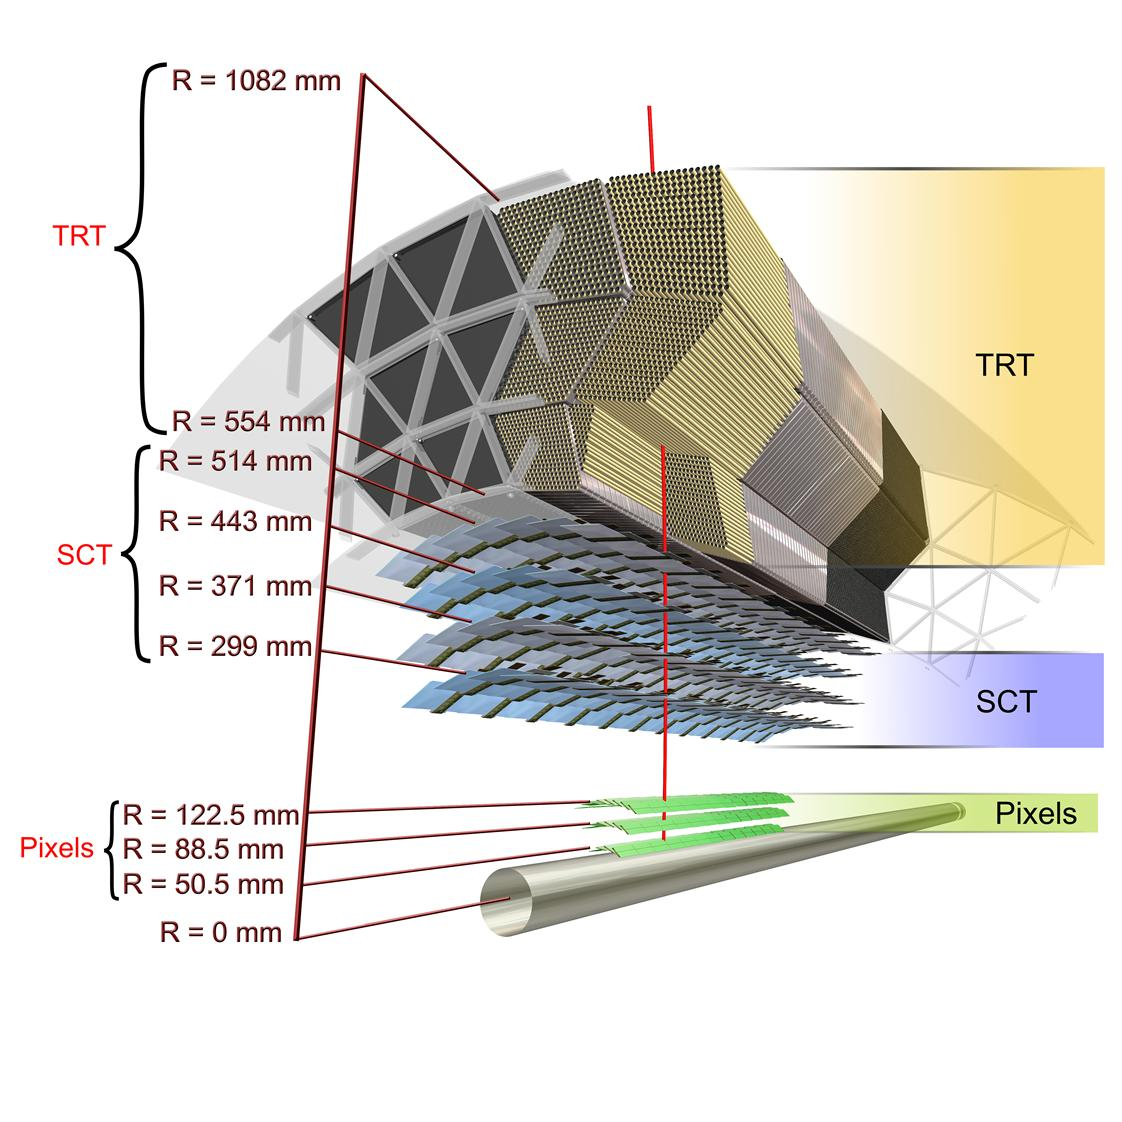
\includegraphics{figures/experiment/ATLAS_ID_track_barrel}}
	}
	\hfill
	\subfloat[ Trajectories of $10 \GeV$ charged particles with $\eta=1.4$ and $\eta=2.2$ traversing the barrel and end-cap elements of the inner detector.] {
		\vspace{-0.4in}
		\resizebox{0.55\textwidth}{!}{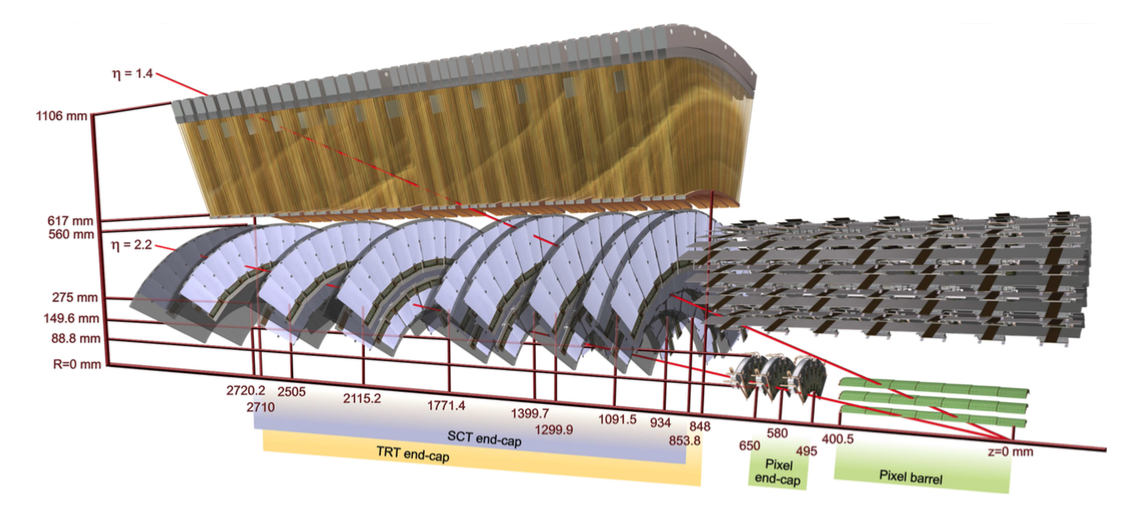
\includegraphics{figures/experiment/ATLAS_ID_track_endcap}}
	}
	\caption{Drawings of the inner detector sensors and structural elements traversed by $10 \GeV$ charged particles originating from the interaction point at various angles.}
	\label{fig:ATLAS-ID-tracks}
\end{figure}


\subsubsection{Pixel Detector}\label{sec:ATLAS-id-pixel-detector}

The pixel detector consists of 1744 identical pixel sensors, each measuring $19\times\SI{63}{\milli\meter\tothe{2}}$ and containing $144\times 328=47232$ pixels, for a total of $80.4\times 10^6$ pixels. The size of the pixels is dictated by the front-end electronics: in 128 of the 144 columns, the pixels have a pitch of $50\times \SI{400}{\micro\meter\tothe{2}}$, while the remaining 16 columns have a pitch of $50\times \SI{600}{\micro\meter\tothe{2}}$. For space reasons, eight pairs of pixels in each column are ganged to a common readout, giving a total of 46080 readout channels per sensor.

 The sensors are $\SI{256}{\micro\meter}$-thick detectors constructed from $n$-type wafers, with high dose positive ($p^+$) and negative ($n^+$) dose regions implanted on each side of a wafer. Initially, the asymmetric depletion region at the $p^+-n$ junction is operated in reverse bias with a voltage of $\SI{150}{\volt}$, and fills the sensor bulk volume, shown in figure~\ref{fig:ATLAS-pixel-normal}. The charge carriers generated by the passage of an ionizing particle through the bulk are collected at the $n^+$ side of the sensor, where the readout electronics are bump-bonded to the pixel. The nominal threshold for readout is about 3,500 electrons, which a minimally ionizing particle cross a pixel leaves a signal of about 20,000 electrons. However, over time, radiation damage induces type inversion in the bulk, after which the junction moves to the $n^+$ side of the sensor and the depletion zone grow from the pixel side, as shown in figure~\ref{fig:ATLAS-pixel-inverted}. The double-sided construction thus allows the pixel sensors to continue operating after type inversion.

 \begin{figure}[htbp]
 	\centering
 	\subfloat[ Before type inversion.] {\label{fig:ATLAS-pixel-normal}
 		\resizebox{0.45\textwidth}{!}{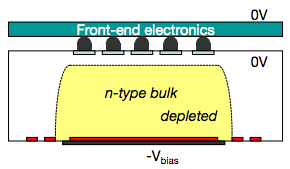
\includegraphics{figures/experiment/ATLAS_pixel_depletion_zones_normal}}
 	}
 	\hfill
 	\subfloat[ After type inversion.] {\label{fig:ATLAS-pixel-inverted}
 		\resizebox{0.45\textwidth}{!}{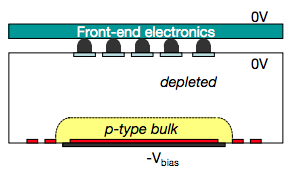
\includegraphics{figures/experiment/ATLAS_pixel_depletion_zones_inverted}}
 	}
 	\caption{Comparison of depletion zones in $n^+$-in-$n$ pixel sensors before and after type inversion. Before type inversion, the electrical field grows from the bottom side, reaching the pixel implants at full depletion. After type inversion, the depletion zone grows from the pixel side, allowing operation even if the bulk is not fully depleted.}
 	\label{fig:ATLAS-pixel}
 \end{figure}

 \begin{figure}[htbp]
 	\centering
 	\resizebox{0.5\textwidth}{!}{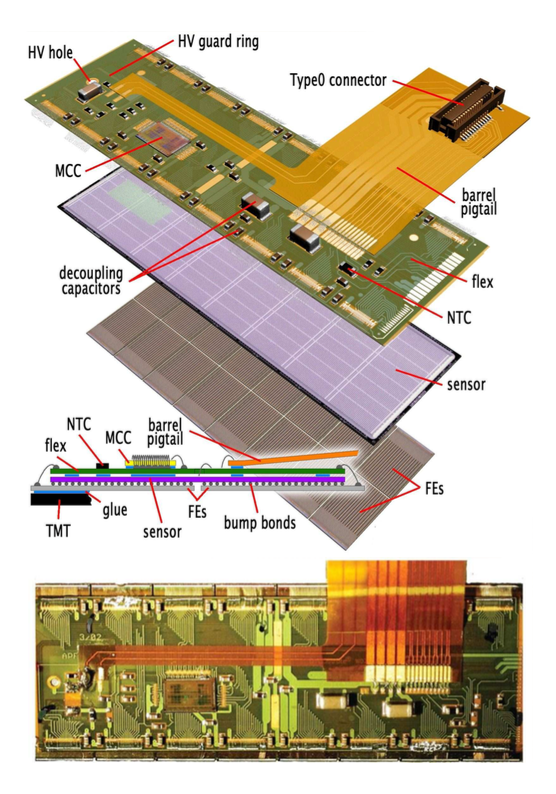
\includegraphics{figures/experiment/ATLAS_pixel_module}}
 	\caption{Schematic pictures of a barrel pixel module. The top diagram shows the assembly of a module, consisting of the front-end electronics chips (FEs), the pixel sensor elements, and the flex-hybrid, which bears the module control chip (MCC) and NTC thermistors. The bottom is a photograph of a barrel pixel module.}
 	\label{fig:ATLAS-pixel-module}
 \end{figure}
 
 

The pixel sensors are assembled into pixel modules, shown in figure~\ref{fig:ATLAS-pixel-module}. Each modules contains 16 front-end electronics chips each with 2880 electronics channels. The front-ends are bump bonded to the pixel sensor elements. The other side of the pixel sensor tile is glued to a flexible polyimide printed circuit board (\emph{flex-hybrid}) that houses the module control chip.

The layout of the pixel detector is summarized in table~\ref{table:ATLAS-pixel-layout}.  The modules are assembled into staves in the barrel region, each with 13 pixel modules, and sectors in the end-caps, each with 6 pixel modules. The barrel layers consist of 22, 38, and 52 staves for layers 0, 1, and 2, respectively, while the end-caps each contain eight sectors. In the barrel, to provide complete coverage, the pixel staves overlap and are mounted with a tilt angle of $20^{\circ}$ between the normal to the module surface and $\hat{r}$, in the $\hat{\phi}$ direction. 

In the barrel, the pixels have an intrinsic accuracy of $\SI{10}{\micro\meter}$ in the $R-\phi$ direction and $\SI{115}{\micro\meter}$ in the $z$ direction, while in the end-caps, the intrinsic accuracy is $\SI{10}{\micro\meter}$ in the $R-\phi$ direction and $\SI{115}{\micro\meter}$ in the $R$ direction.

\begin{table}[htbp]
	\centering
	\begin{tabular}{|l|c|c|c|c|}
		\hline
		\textbf{Barrel} & \textbf{Radius (mm)} & \textbf{Modules} & \textbf{Pixels} \\
		\hline
		Layer-0 & $50.5$ & $22$ & $286$ & $13.2\times 10^6$ \\
		Layer-1 & $88.5$ & $38$ & $494$ & $22.8\times 10^6$ \\
		Layer-2 & $112.5$ & $52$ & $676$ & $31.2\times 10^6$ \\
		\hline
		\textbf{End-cap (one side)} & $z$ \textbf{(mm)} & \textbf{Sectors} & \textbf{Modules} & \textbf{Pixels} \\
		\hline
		Disk 1 & $495$ & $8$ & $48$ & $2.2\times 10^6$ \\
		Disk 2 & $495$ & $8$ & $48$ & $2.2\times 10^6$ \\
		Disk 3 & $495$ & $8$ & $48$ & $2.2\times 10^6$ \\
		\hline
		\textbf{Barrel and both end-caps} & & $1744$ & $80.4\times 10^6$ \\
		\hline
	\end{tabular}
	\caption{Parameters of the pixel detector, from~\cite{TheATLASCollaboration:2008fg}.}
	\label{table:ATLAS-pixel-layout}
\end{table}

\subsubsection{SCT}\label{sec:ATLAS-id-sct}

The SCT consists of 15912 sensors using single-sided, p-in-n type silicon strips. The use of single-sided strips lowers both the cost and the number of readout channels of the detector, which covers significantly more area than the pixel detector ($\SI{61.1}{\meter\tothe{2}}$ versus $\SI{2.3}{\meter\tothe{2}}$). In the barrel, the strips have a pitch of $\SI{80}{\micro\meter}$ and a length of $\SI{12}{\centi\meter}$. In the endcaps, the sensors are trapezoidal with radially arranged strips, with a mean strip pitch of $\SI{80}{\micro\meter}$ and a length of $\SI{12}{\centi\meter}$. Each sensor has 768 active strips. Like the pixel sensors, the operating voltage will be $\sim$\SI{150}{\volt} initially, and will increase to \SIrange[range-phrase=-]{250}{350}{\volt} after several years of irradiation, depending on the location of the sensor. 

The SCT modules are shown in figure~\ref{fig:ATLAS-SCT-modules}.The 2112 barrel modules contain four sensors, while the 1976 end-cap modules contain two sensors. In both cases, the sensors are glued to a $\SI{380}{\micro\meter}$-thick thermal pyrolitic graphite (TPG) base-board. The sensors are assembled in two layers with a rotation of $\pm\SI{20}{\milli\radian}$ about the center of the sensors. The stereo angle between the two sensors allows for a measurement of the position along the length of the sensors. 

% Arrangement into barrel layers and end-caps

The intrinsic accuracy of the SCT sensors is $\SI{17}{\micro\meter}$ along the strip pitch, corresponding to the $R-\phi$ direction. Along the length of the strips, the stereo angle allows for position measurement with an accuracy of $\SI{580}{\micro\meter}$, corresponding to the $z$ direction in the barrel and the $R$ direction in the end-caps.

\begin{table}[htbp]
	\centering
	\scriptsize
	\begin{tabular}{|l|c|c|c|c|}
		\hline
		\textbf{Barrel layer} & \textbf{Radius (mm)} & \textbf{Length (mm)} & \textbf{Module tilt angle} & \textbf{Number of modules} \\
		\hline
		3 & $299$ & $1498$ & $11.00^{\circ}$ & $384$ \\
		4 & $371$ & & $11.00^{\circ}$ & $480$ \\
		5 & $443$ & & $11.25^{\circ}$ & $576$ \\
		6 & $514$ & & $11.25^{\circ}$ & $672$ \\
		\hline
	\end{tabular}
	\caption{The dimensions and arrangement of modules in the four SCT layers. The tilt angle is between the normal to the module surface and $\hat{r}$, in the $\hat{\phi}$ direction.}
	\label{fig:ATLAS-SCT-layout}
\end{table}

\subsubsection{TRT}\label{sec:ATLAS-id-trt}

The TRT detector elements are polyimide drift (straw) tubes. The straws are arranged such that charged particles with $\pt > \SI{500}{\mega\electronvolt}$ and $|\eta|<2.0$ traverse at least 36 straws, except in the barrel/end-cap transition region where particles traverse as few as 22 straws. The straws are interleaved with polypropylene fibers in the barrel and polypropylene foils in the end-caps to provide transition radiation; electrons with $\pt>\SI{2.0}{\giga\electronvolt}$ typically leave $7$-$10$ high-threshold hits. The intrinsic resolution of the straws is $\SI{130}{\micro\meter}$ in the transverse direction.

The straws measure $\SI{4}{\milli\meter}$ in diameter and $\SI{144}{\centi\meter}$ ($\SI{37}{\centi\meter}$) in length in the barrel (end-caps). The straw walls consist of two $\SI{35}{\micro\meter}$ films bonded back-to-back. The base film material is a $\SI{25}{\micro\meter}$ thick layer of polyamide, which is coated on the exterior side with a $\SI{0.2}{\micro\meter}$ thick layer of Al and a \SIrange[range-phrase=-]{5}{6}{\micro\meter} thick protective layer of graphite-polyamide. The other side of the film is coated with a \SIrange[range-phrase=-]{5}{6}{\micro\meter} thick layer of polyurethane, which is used to heat-seal the two film layers together. The anodes of the detectors are tungsten wires running down the axis of the tubes, with $\SI{31}{\micro\meter}$ diameter and plated with \SIrange[range-phrase=-]{0.5}{0.7}{\micro\meter} of gold. The wires are supported at the end of the straw by an end plug, where they connect to the front-end electronics. At the middle of the straw, the wires are supported by a plastic insert, and are also split electrically by a fused glass capillary to reduce occupancy. The active length of each half of the wire is $\SI{71.2}{\centi\meter}$, with a $\SI{2}{\centi\meter}$ inefficient length at the middle. The signal attenuation length is $\sim$\SI{4}{\meter}, and the signal propagation time is $\sim$\SI[per-mode=fraction]{4}{\nano\second\per\meter}. The straws are filled with a mixture of 70\% Xe, 27\% CO$_2$, and $3\%$ O$_2$. With a cathode voltage of $\SI{-1530}{\volt}$, the gain in the straws is $2.5\times 10^4$.

The layout of the straws in the barrel and end-caps is summarized in table~\ref{table:ATLAS-TRT-layout}. In the barrel, the straws are arranged into three layers of modules as shown in figure~\ref{fig:barrel-modules}, with different dimensions and straw counts depending on the layer. The straws are interleaved with transition radiation material, polypropylene fibers measuring $\SI{19}{\micro\meter}$ in diameter. The module shell is made from $\SI{400}{\micro\meter}$ thick carbon fiber, and serve not only as a support structure, but also as a gas manifold for CO$_2$, which prevents high-voltage discharges, flushes any Xe leaking from the straws, and conducts heat away from the straws.  

The endcaps consist of 160 layers of 768 straws, arranged radially into 20 wheels with 8 layers each. The inner 12 wheels (type-A) are spaced $\SI{8}{\milli\meter}$ in $z$, while the outer 8 wheels (type-B) are spaced by $\SI{15}{\milli\meter}$. Each successive layer in a wheel is separated by a $\SI{15}{\micro\meter}$ thick polypropylene radiator foil, and is rotated by $3/8$ of the azimuthal straw spacing to optimize the uniformity of the number of straw crossed.


\begin{table}[htbp]
	\centering
	\begin{tabular}{|l|c|c|c|c|c|}
		\hline
		 & $z$ (mm) & $R$ (mm) & Modules & Layers & Straws/Module \\
		 \hline
		 \textbf{Barrel (both sides)} & $\mathbf{0\mhyphen780}$ & $\mathbf{554\mhyphen1082}$ & $\mathbf{96}$ & $\mathbf{73}$ & $\mathbf{52544}$ \\
		 Type-1 module (inner) & $400\mhyphen712.1$ & $563\mhyphen624$ & \multirow{2}{*}{$32$} & $9$ & \multirow{2}{*}{$329$} \\
		 Type-1 module (outer) & $7.5\mhyphen712.1$ & $625\mhyphen 694$ & & $10$ & \\
		 Type-2 module & $7.5\mhyphen 712.1$ & $697\mhyphen860$ & $32$ & $24$ & $520$ \\
		 Type-3 module & $7.5\mhyphen 712.1$ & $863\mhyphen 1066$ & $32$ & $30$ & $793$ \\
		 \hline
		 \textbf{End-cap (one side)} & $\mathbf{827\mhyphen 2744}$ & $\mathbf{615\mhyphen1106}$ & $\mathbf{20}$ & $\mathbf{160}$ & $\mathbf{122880}$ \\
		 Type-A wheels & $848\mhyphen1705$ & $644\mhyphen1004$ & $12$ & $8$ & $6144$ \\
		 Type-B wheels & $1740\mhyphen2710$ & $644\mhyphen1004$ & $8$ & $8$ & $6144$ \\
		 \hline
	\end{tabular}
	\caption{Layout and straw counts of the TRT barrel modules and end-cap wheels. The totals for the barrel and end-caps, shown in bold, include services and electronics.}	
	\label{table:ATLAS-TRT-layout}
\end{table}


\subsection{Calorimetry}\label{sec:ATLAS-calorimeters}
The calorimeter system occupies the volume directly exterior to the solenoid magnet, and measures the energy of electrons, photon, and hadrons up to a pseudorapidity of $|\eta|=4.9$. The arrangement of the calorimeters is shown in figure~\ref{fig:ATLAS-calorimeters}. The system consists of a number of independent sampling calorimeters. The electromagnetic calorimeter measures the energy of electrons and photons using lead and liquid argon (LAr) to measure the energy of electrons and photons. The hadronic calorimeter measures the energy of hadrons using steel and scintillator tiles in the barrel and copper and LAr in the end-caps. Finally, electromagnetic and hadronic calorimetry is performed in the forward region using copper-LAr and tungsten-LAr technology. Besides performing energy measurements, the calorimeters providing containment electrons, photons, and hadrons, which effectively provides shielding for the muon spectrometer~\ref{sec:ATLAS-muon-spectrometer}. The total amount of material in front of and in the calorimeters is shown in terms of radiation lengths, $X_0$, and interaction lengths, $\lambda$, in figures~\ref{fig:ATLAS-calorimeters-X0} and \ref{fig:ATLAS-calorimeters-lambda0}.

\begin{figure}[htbp]
	\centering
	\resizebox{0.7\textwidth}{!}{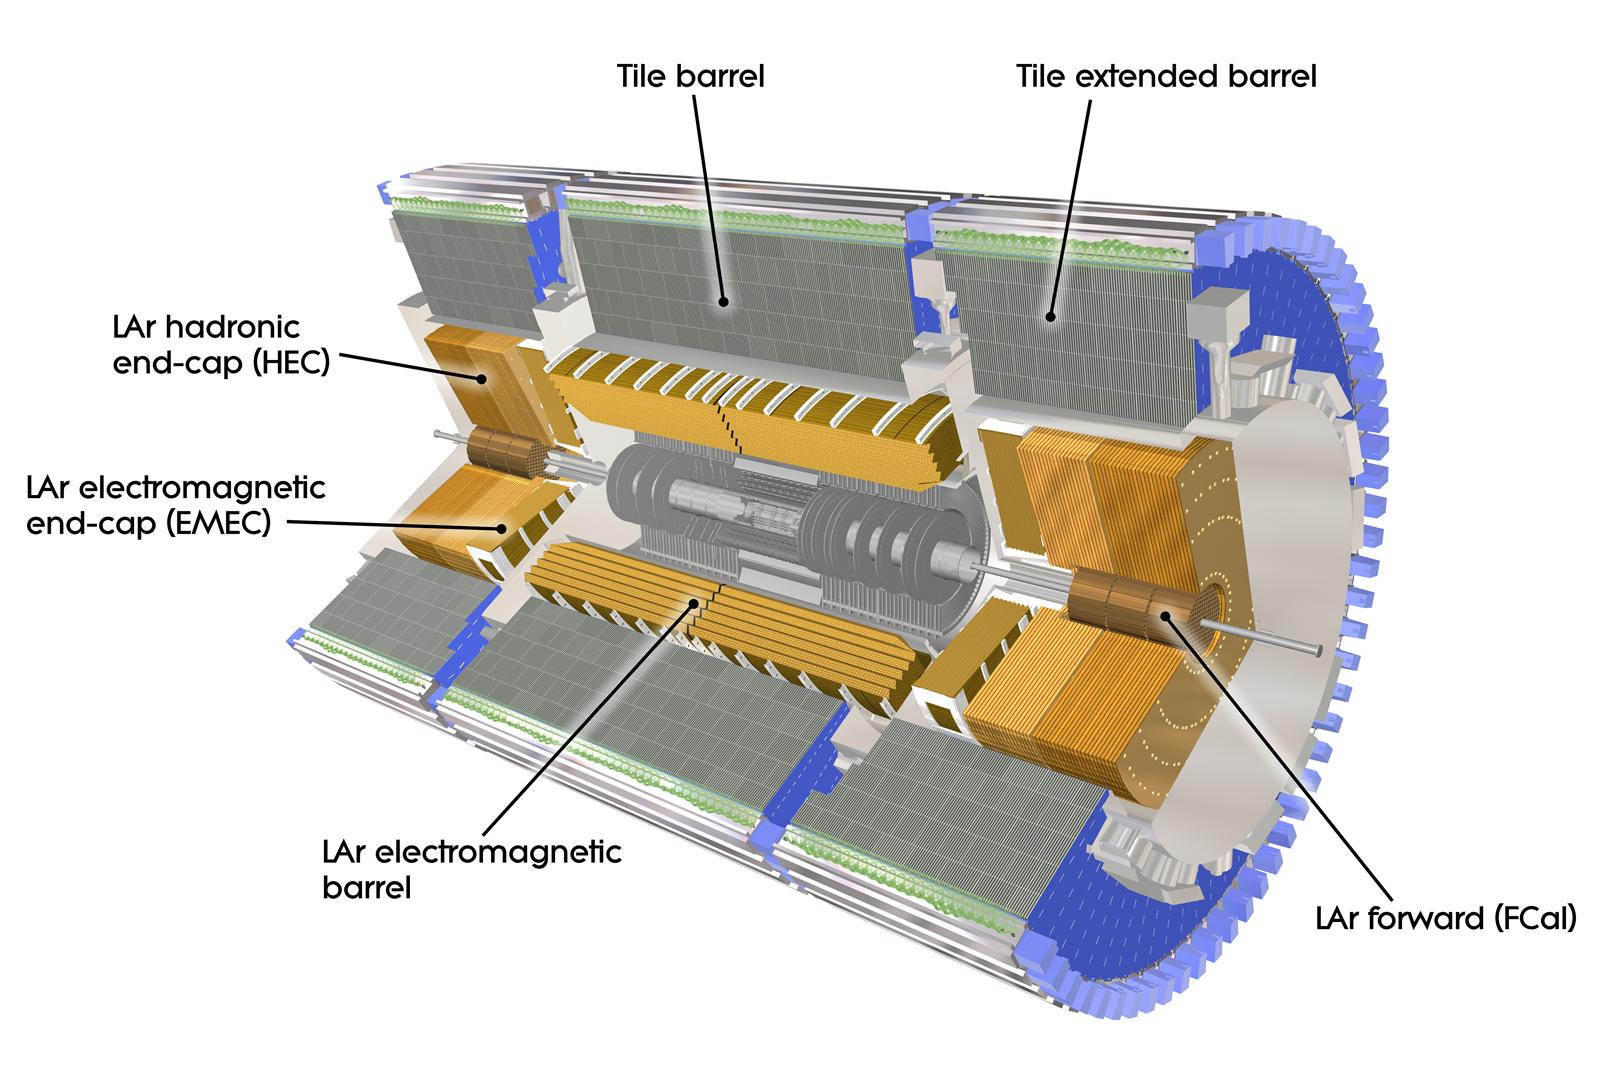
\includegraphics{figures/experiment/ATLAS_calorimeters_sketch}}
	\caption{A 3D model of the ATLAS calorimeters, showing the electromagnetic barrel and end-caps, hadronic barrel and end-caps, and the forward calorimeter.}
	\label{fig:ATLAS-calorimeters}
\end{figure}

\begin{figure}
	\centering
	\subfloat[ Material before the calorimeters.] {
		\resizebox{0.45\textwidth}{!}{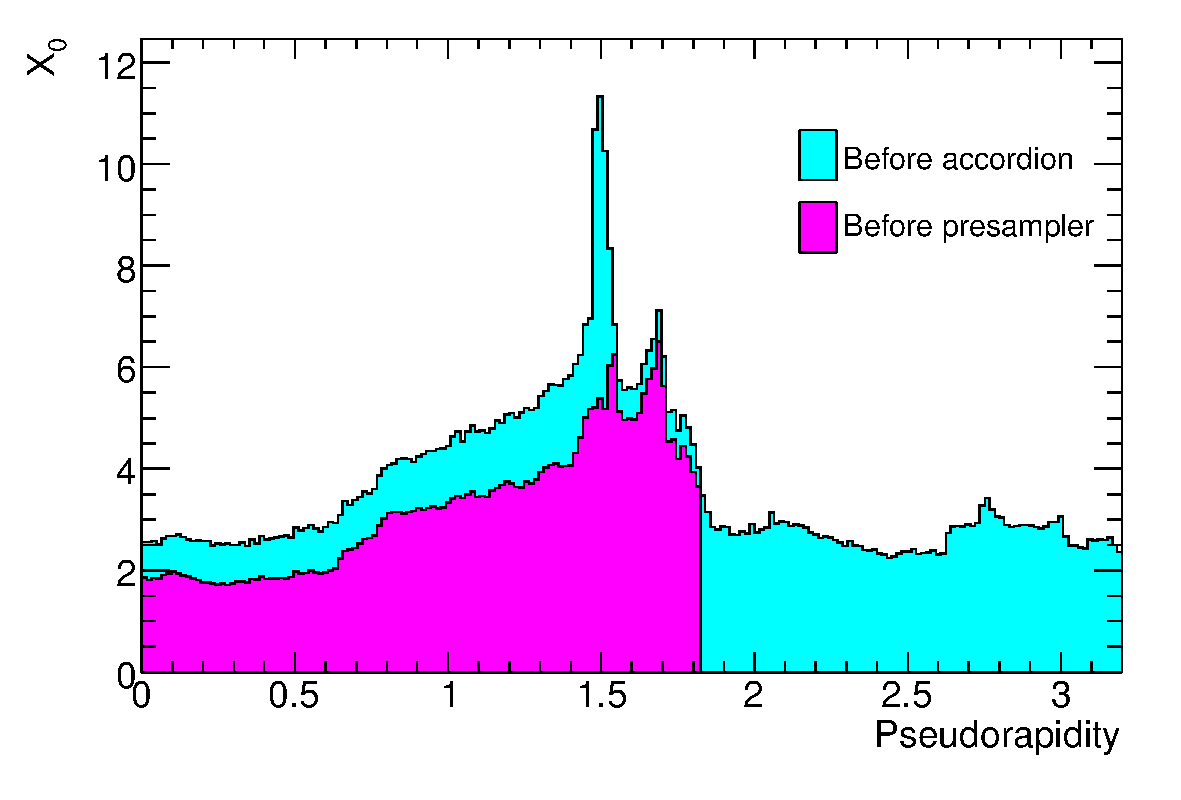
\includegraphics{figures/experiment/x0_before_calo_csc03}}
	}\hfill
	\subfloat[ Material in the crack region between the barrel and end-cap cryostats.] {
		\resizebox{0.45\textwidth}{!}{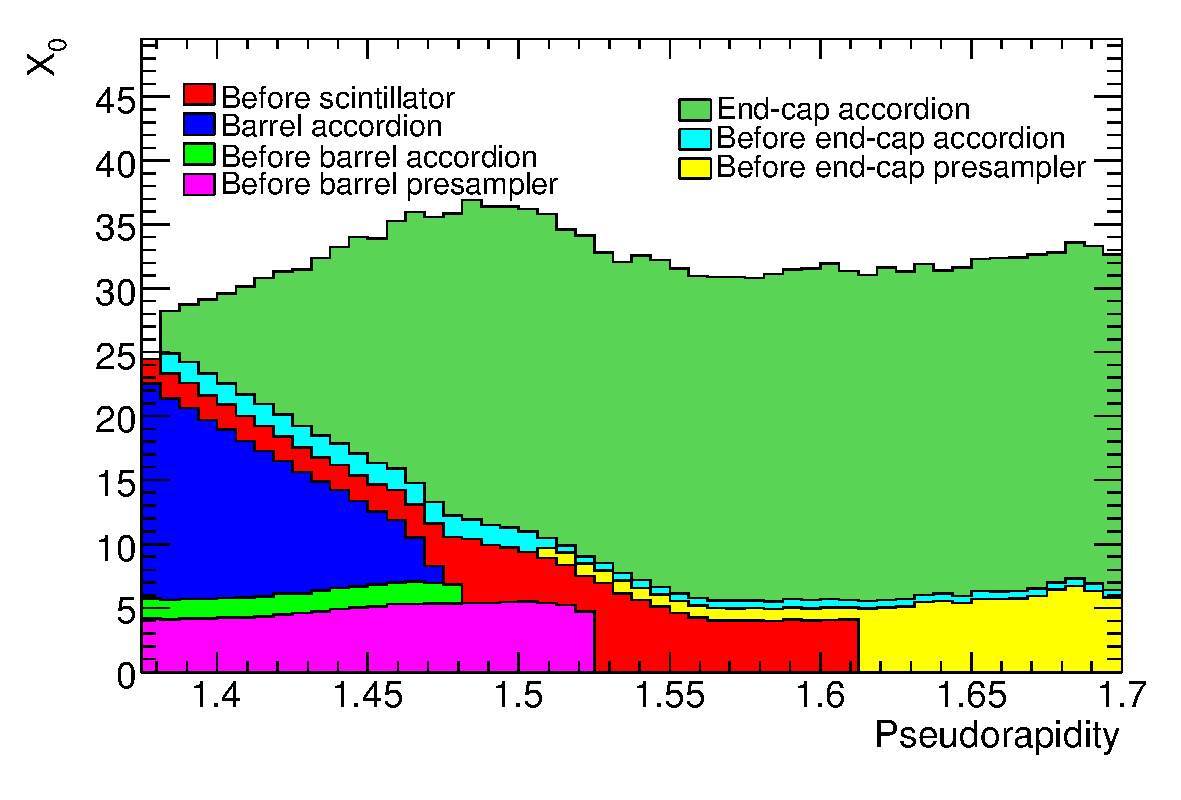
\includegraphics{figures/experiment/x0_crack_csc03}}
	} \\
	\subfloat[ Material in and before the barrel LAr calorimeter.] {
		\resizebox{0.45\textwidth}{!}{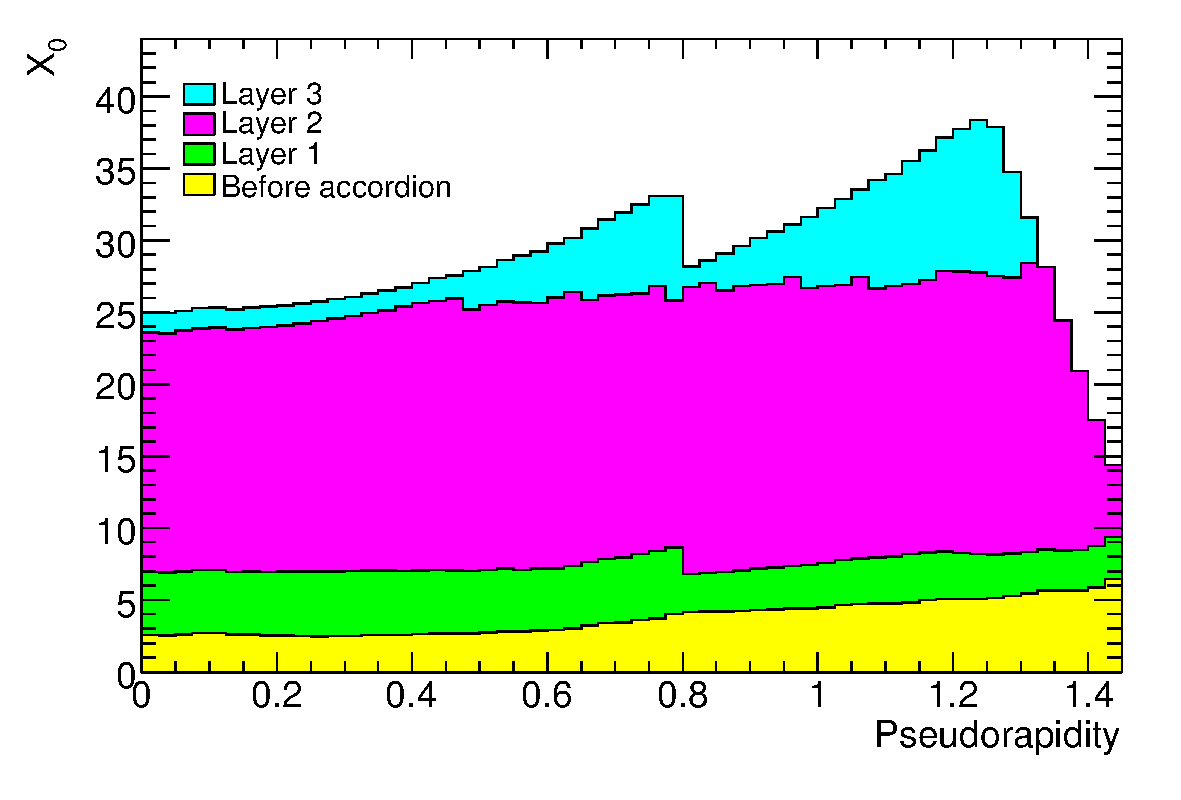
\includegraphics{figures/experiment/x0_layers_barrel_csc03}}
	}\hfill
	\subfloat[ Material in and before the end-cap LAr calorimeters.] {
		\resizebox{0.45\textwidth}{!}{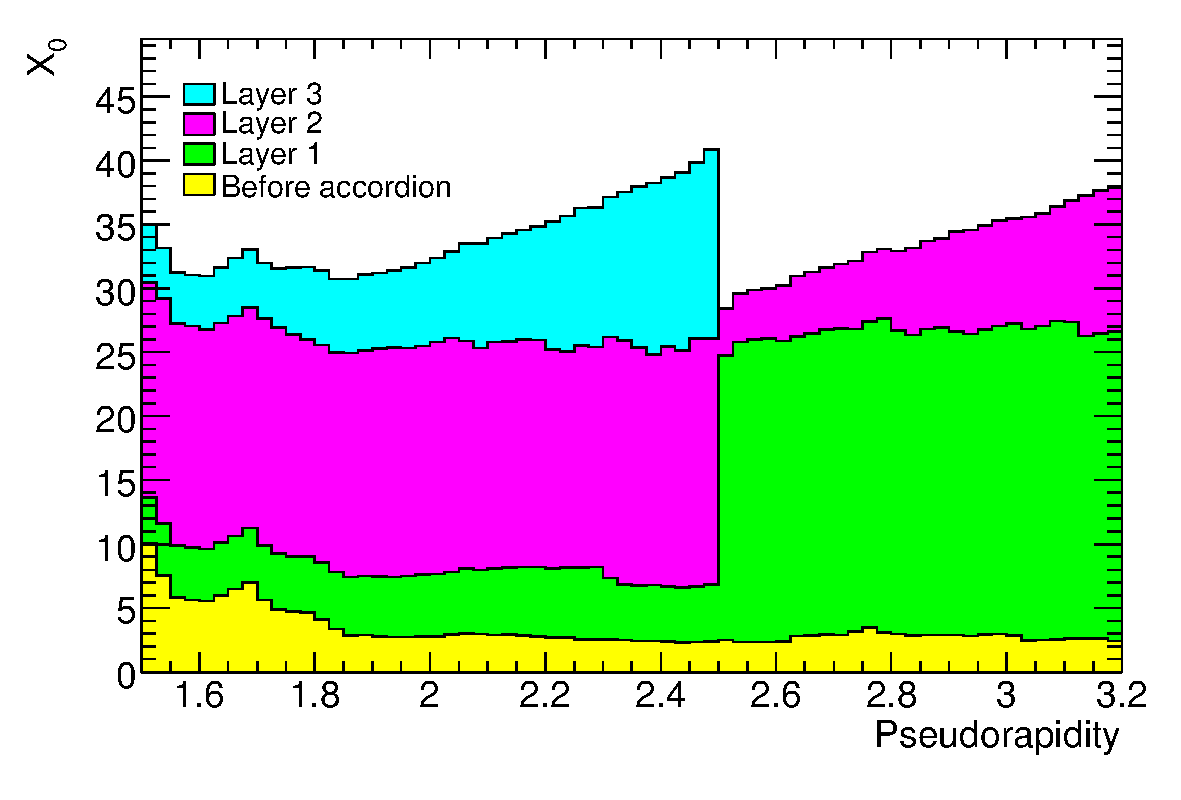
\includegraphics{figures/experiment/x0_layers_endcap_csc03}}
	}
	\caption{Cumulative amounts of material versus $|\eta|$ in front of and within the LAr electromagnetic calorimeter, in terms of radiation lengths, $X_0$.}
	\label{fig:ATLAS-calorimeters-X0}
\end{figure}

\begin{figure}
	\centering
	\resizebox{0.6\textwidth}{!}{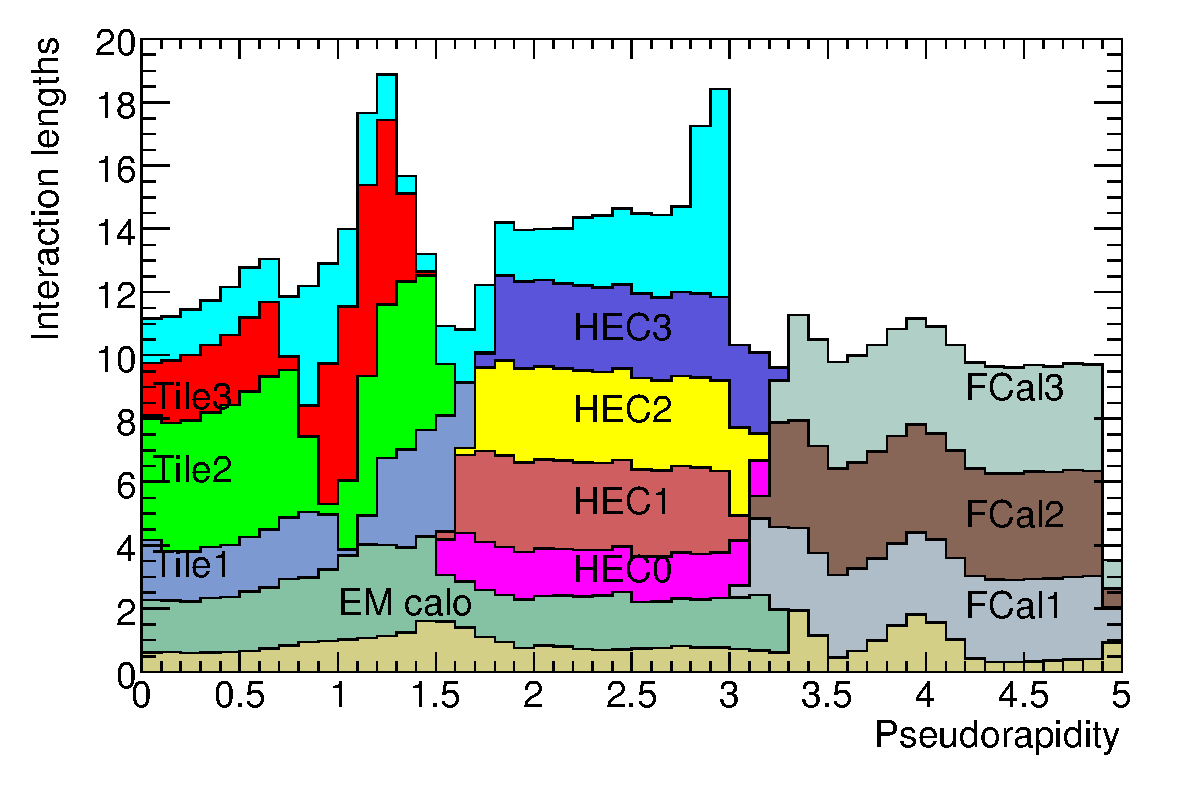
\includegraphics{figures/experiment/lambda_csc03}}
	\caption{Cumulative amounts of material versus $|\eta|$ due to each calorimeter in terms of interaction lengths, $\lambda$. The material in front of the calorimeters is also shown in tan.}
	\label{fig:ATLAS-calorimeters-lambda0}
\end{figure}



\subsubsection{Electromagnetic Calorimeter}\label{sec:ATLAS-calorimeters-ecal}

The electromagnetic calorimeter consists of two half-barrels ($0<\eta<\pm1.475$) and two end-caps ($1.375<|\eta|<3.2$), all of which use LAr as the active material and steel-clad lead plates as the absorber. The lead plates are arranged in an accordion geometry to provide a uniform, gapless coverage in $\phi$, shown for a barrel module in figure~\ref{fig:ATLAS-LAr-module}. The plates are interleaved with electrodes built from copper etchings on polymide, consisting of three conducting layers. The outer conductive layers of the electrodes distribute the $\SI{2000}{\volt}$ high voltage over the electrode surface, which drifts the charges induced by ionization in the LAr towards the electrodes with a drift time of $\SI{450}{\nano\second}$. The inner layer of the electrode, separated from the outer layers by isolating foils, collects the signals via capacitive coupling.

\begin{figure}[htbp]
	\centering
	\subfloat[ A LAr barrel module.] {
		\resizebox{0.45\textwidth}{!}{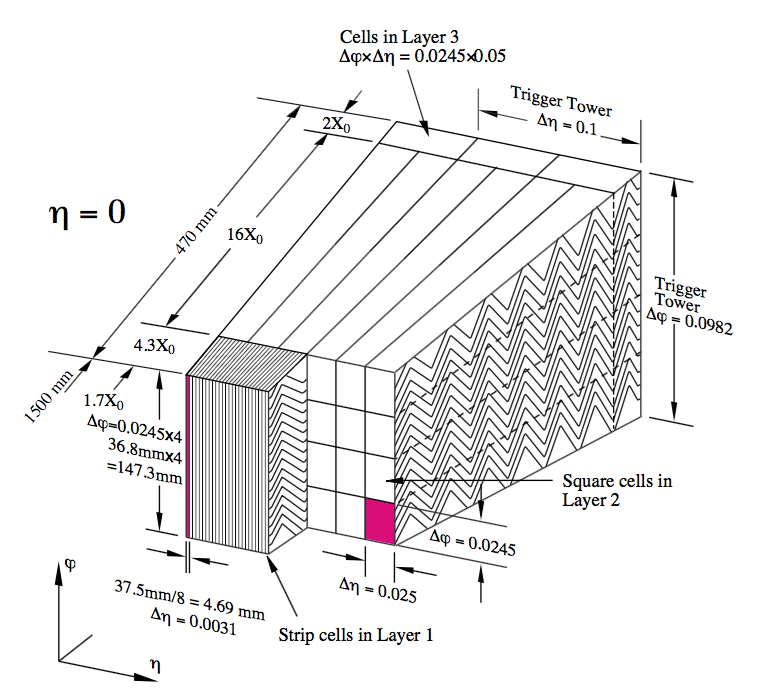
\includegraphics{figures/experiment/ATLAS_LAr_module}}
	}
	\subfloat[ Closeup image of the LAr accordion geometry.] {
		\resizebox{0.45\textwidth}{!}{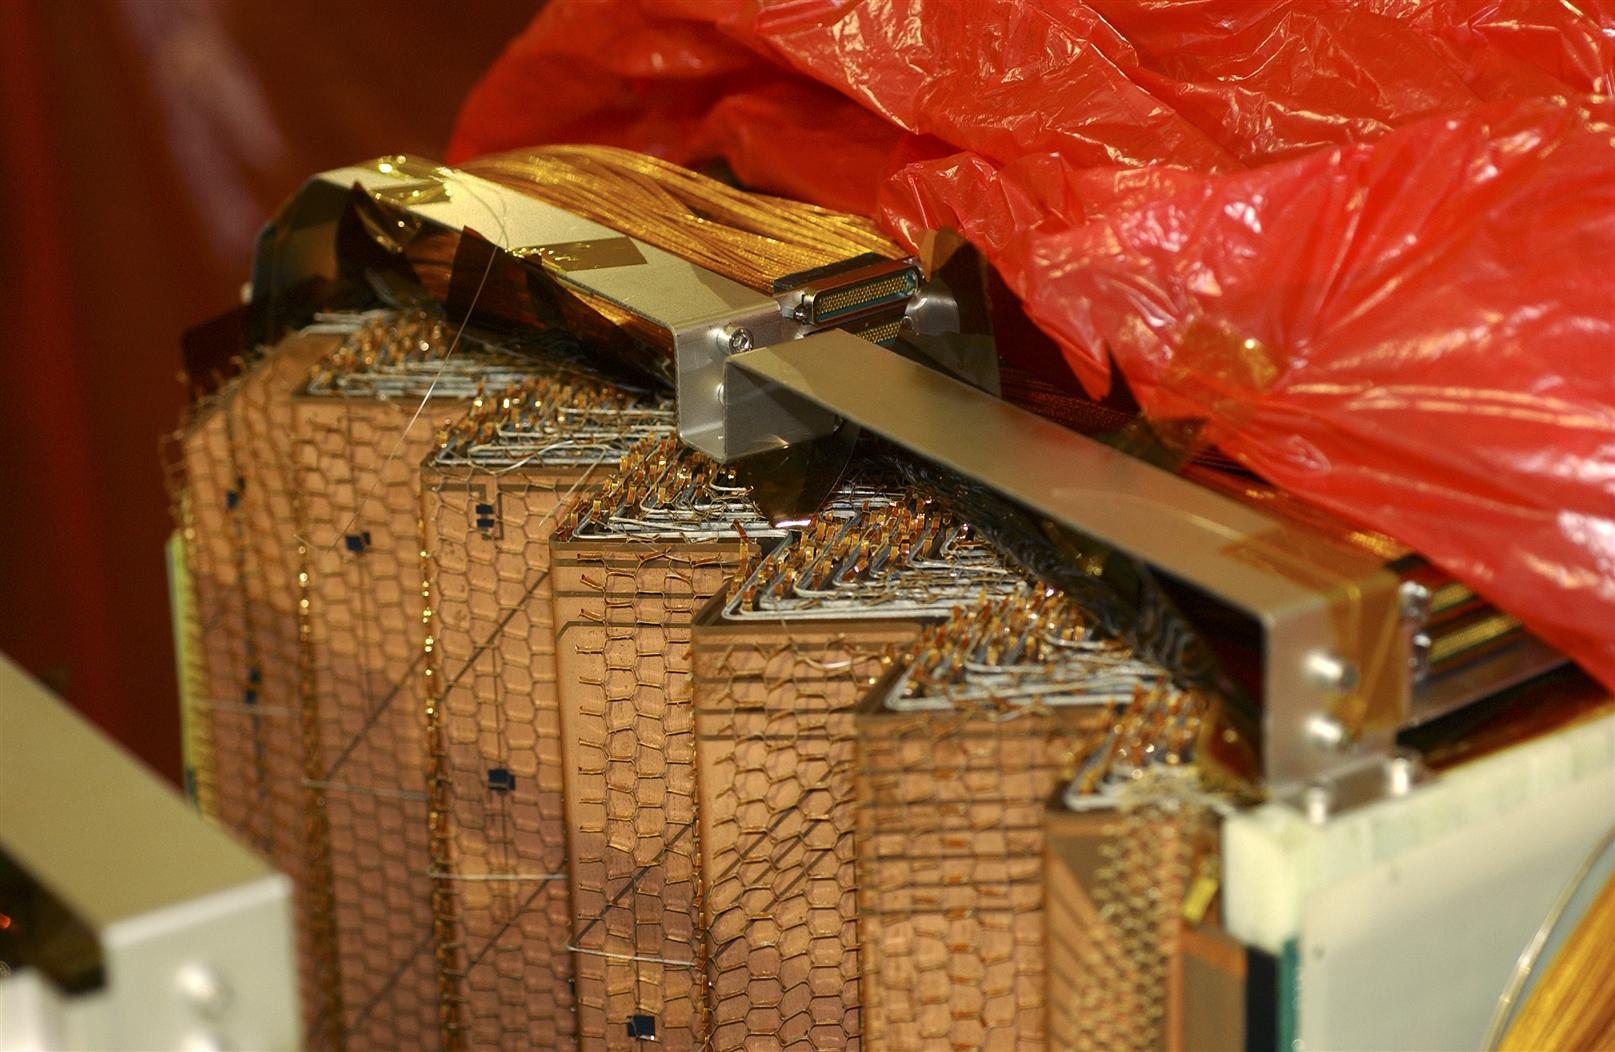
\includegraphics{figures/experiment/ATLAS_LAr_zigzags}}
	}
	\caption{The LAr calorimeter uses an accordion geometry to provide uniform coverage in $\phi$. Steel-clad lead plates are interleaved with electrodes, consisting of three copper layers separated by polyamide sheets. The barrel module is divided into three layers in depth, with fine segmentation in $\eta$ in the layer closest the interaction point.}
	\label{fig:ATLAS-LAr-module}
\end{figure}


The two half-barrels occupy the region $\SI{2.8}{\meter}<R<\SI{4}{\meter}$ and $\SI{0}{\meter}<z<\pm\SI{3.2}{\meter}$. Each has 1024 lead plates with a thickness of $\SI{1.53}{\milli\meter}$ for $|\eta|<0.8$ and $\SI{1.13}{\milli\meter}$ for $|\eta|>0.8$. The barrels are divided into 16 modules, each covering an azimuthal angle of $\Delta \phi = 22.5^{\circ}$. Each module has three layers in depth to provide a rough measurement of the longitudinal profile of the electromagnetic showers. The segmentation of each layer in $\Delta\eta\times\Delta\phi$ is shown in table~\ref{table:ATLAS-LAr-segmentation}. The fine segmentation of the front layer aids particle identification, and, in combination with the middle layer, allows for a measurement of photon trajectories. A LAr half barrel is shown in figure~\ref{fig:LAr-barrel}, prior to installation.

\begin{figure}[htbp]
	\centering
	\resizebox{0.4\textwidth}{!}{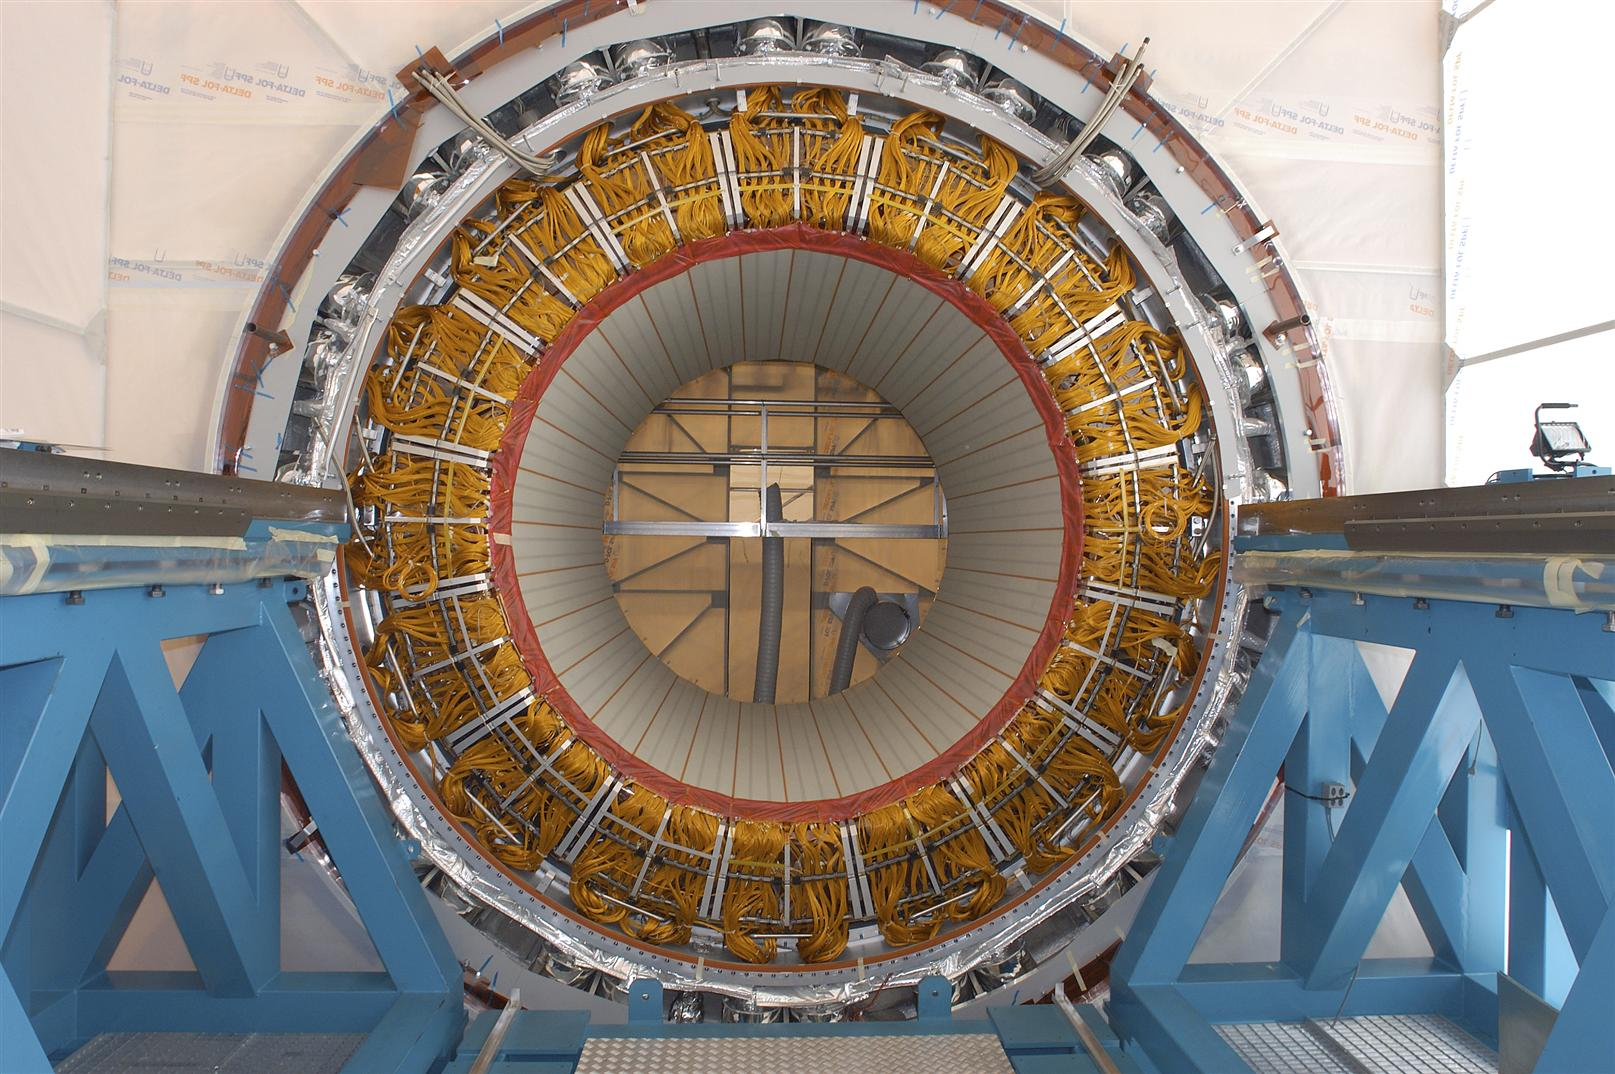
\includegraphics{figures/experiment/ATLAS_LAr_barrel}}
	\caption{Photograph of a LAr calorimeter half-barrel, prior to installation.}
	\label{fig:LAr-barrel}
\end{figure}


The end-caps, one on either side of the interaction region, measure $\SI{63}{\centi\meter}$ in thickness with inner and outer radii of $\SI{33}{\centi\meter}$ and $\SI{209.8}{\centi\meter}$, respectively. Each end-cap contains two co-axial sub-wheels, divided by a $\SI{3}{\milli\meter}$ gap at $|\eta|=2.5$. The inner and outer wheels contain 256 and 768 lead absorbers, respectively, with the same accordion geometry as used in the barrel. In the region $1.5<|\eta|<2.5$, the outer wheel of the end-caps presents three layers in the longitudinal direction, with fine $\eta$ segmentation in the front layer. For $|\eta|<1.5$ in the outer wheel and the entire inner wheel ($2.5<|\eta|<3.2$), there are two longitudinal layers and coarser transverse granularity.

The total amount of material before and in the electromagnetic calorimeters is shown in figure~\ref{fig:ATLAS-calorimeters-X0} in terms of radiation lengths, $X_0$. The beam pipe, inner detector, solenoid, cryostats, and other services and support structures present a significant amount of material in between the interaction point and the calorimeters. To provide a measurement of the energy loss due to particles interacting before the calorimeters, a presampler is installed in front of the first LAr layer. The presampler is a liquid argon layer $\SI{11}{\milli\meter}$ in depth, divided into 64 azimuthal sectors (32 in each half-barrel) of dimension $\Delta\eta\times\Delta\phi=1.52\times0.2$. Each sector contains eight modules, the central seven of which span $\Delta\eta=0.2$, and the outermost of which measures $\Delta\eta=0.12$.  The modules contain interleaved cathodes and anodes with \SIrange[range-phrase=-]{1.9}{2.0}{\milli\meter} spacing. Like the three LAr calorimeter layers, the anodes contain three conducting layers, the outer two of which supply the $\SI{2000}{\volt}$ operating voltage, and the innermost of which performs the signal readout via capacitive coupling.

% Conclusion
In total, the electromagnetic calorimeter has 101,760 readout channels for the barrel, 62,208 channels for the end-caps, 7,808 channels for the barrel presampler, and 1,536 channels for the end-cap presamplers. 


\begin{table}[htbp]
	\centering
	\begin{tabular}{|l|c|c|}
		\hline
		Layer & $\eta$ range & Granularity $\Delta\eta\times\Delta\phi$ \\
		\hline
		Barrel presampler & $|\eta|<1.52$ & $0.025\times0.1$ \\
		\hline
		\multirow{2}{*}{Barrel 1} & $|\eta|<1.40$ & $0.025 / 8 \times 0.1$ \\
		 & $1.40<|\eta|<1.475$ & $0.025\times0.025$ \\
		\hline
		\multirow{2}{*}{Barrel 2} & $|\eta|<1.40$ & $0.025\times0.025$ \\
		 & $1.40<|\eta|<1.475$ & $0.075\times 0.025$ \\
		\hline
		Barrel 3 & $|\eta|<1.35$ & $0.050\times0.025$ \\
		\hline
		\hline
		\multirow{7}{*}{End-cap 1} & $1.375<|\eta|<1.425$ & $0.050\times0.1$ \\
		 & $1.425<|\eta|<1.5$ & $0.025\times0.1$ \\
		 & $1.5<|\eta|<1.8$ & $0.025/8\times0.1$ \\
		 & $1.8<|\eta|<2.0$ & $0.025/6\times0.1$ \\
		 & $2.0<|\eta|<2.4$ & $0.025/4\times0.1$ \\
		 & $2.4<|\eta|<2.5$ & $0.025\times0.1$ \\
		 & $2.5<|\eta|<3.2$ & $0.1\times0.1$ \\
		\hline
		\multirow{3}{*}{End-cap 2} & $1.375<|\eta|<1.425$ & $0.050\times0.025$ \\
		 & $1.425<|\eta|<2.5$ & $0.025\times0.025$ \\
		 & $2.5<|\eta|<3.2$ & $0.1\times0.1$ \\
		\hline
		End-cap 3 & $1.5<|\eta|<2.5$ & $0.050\times0.025$ \\
		\hline
	\end{tabular}
	\caption{Granularity of each layer of the LAr electromagnetic calorimeter.}
	\label{table:ATLAS-LAr-segmentation}
\end{table}


\subsubsection{Tile Calorimeter}\label{sec:ATLAS-calorimeters-tile}
The tile calorimeter performs hadronic calorimetry in the region $|\eta|<1.7$, occupying the radial range $\SI{2.28}{\meter}<R<\SI{4.25}{\meter}$. Divided into a $\SI{5.8}{\meter}$-long central barrel and two $\SI{2.6}{\meter}$-long extended barrels on either side, the tile calorimeter uses steel as the absorber and scintillating tiles as the active material. The total depth is approximately $7.4\lambda$. 

Each of the three calorimeter sections is divided azimuthally into 64 modules, each spanning $\Delta\phi=5.625$. A module is shown schematically in figure~\ref{fig:ATLAS-calorimeters-tile-module}. The outer edge of a module is a steel girder which houses the tile calorimeter readout electronics and also provides flux return for the solenoidal magnetic field. The body of the module is a self-supporting structure built from steel absorber plates, with $\SI{4}{\milli\meter}$-thick spacer plates glued in staggered fashion to $\SI{5}{\milli\meter}$-thick master plates. The staggered spacing creates the gaps into which the scintillating tiles are inserted, with a steel-to-scintillator volume ratio of approximately $4.7:1$. 

The scintillating tiles use polystyrene as the base material, in which ionizing particles induce the production of ultraviolet light. The polystyrene is doped with wavelength-shifting fluors, 1.5\% PTP and 0.044\% POPOP, which convert the scintillation light into the visible light. The tiles measure $\SI{3}{\milli\meter}$ thick, and vary between \SIrange[range-phrase=-]{97}{187}{\milli\meter} in radial length and \SIrange[range-phrase=-]{200}{400}{\milli\meter} in azimuthal length. A plastic sleeve envelops each tile, both for the protection of the tile during installation and also to improve the scintillation light collection efficiency due to a reflectivity of $\sim 95\%$. 

At the tile edges, the light is collected by wavelength-shifting fibers, which transmit the light to photomultiplier tubes housed in the girder. The fibers occupy a gap between adjacent modules approximately $\SI{1.5}{\milli\meter}$ wide. The fibers are grouped to form a three-dimensional sampling structure as shown in figure~\ref{fig:ATLAS-calorimeters-tile-cell-layout}, with cells measuring $\Delta\eta\times\Delta\phi=0.1\times0.1$ in the transverse direction. Longitudinally, the grouping provides three radial sampling layers, with depths at $\eta=0$ of approximately $1.5\lambda$, $4.1\lambda$, and $1.8\lambda$ in order of increasing distance from the interaction point. 

\begin{figure}[htbp]
	\centering
	\subfloat[ Schematic view of a tile calorimeter module, showing assembly of the steel absorber, the inserted scintillator tiles, and the readout of lighting through wavelength-shifting fibers to the photomultiplier tubes.] {\label{fig:ATLAS-calorimeters-tile-module}
		\resizebox{0.4\textwidth}{!}{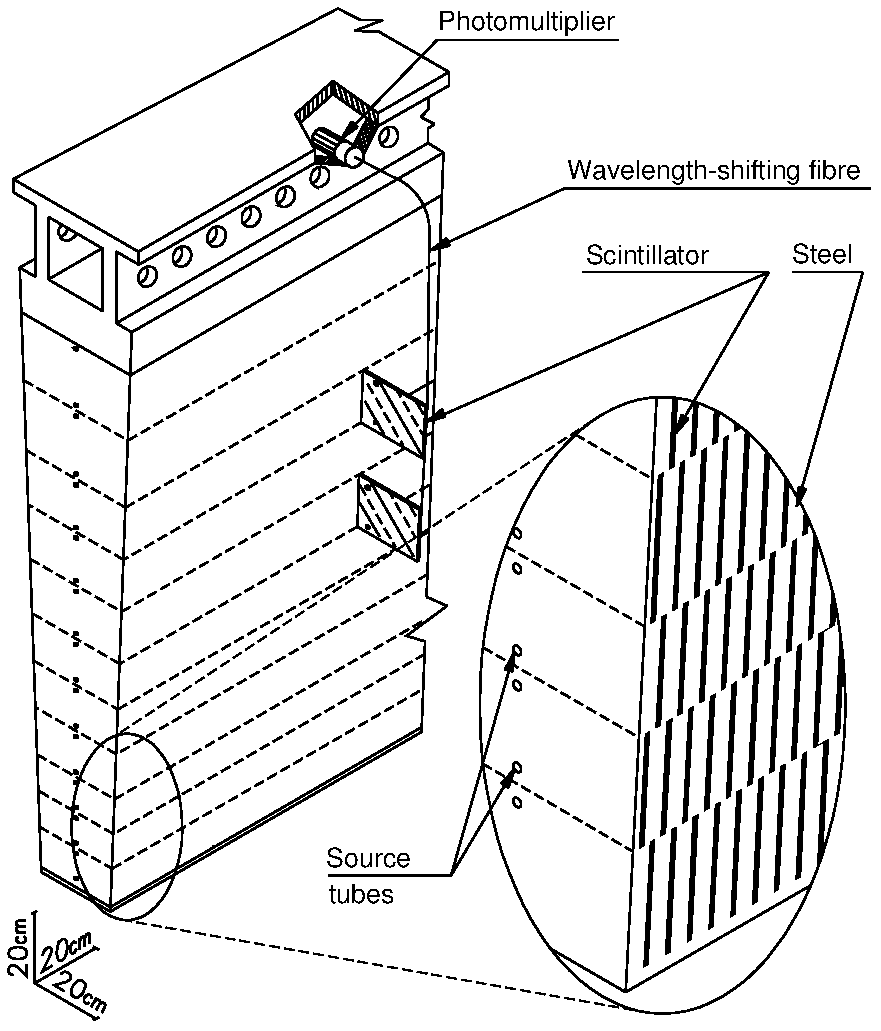
\includegraphics{figures/experiment/ATLAS_TILE_module}}
	}
	\subfloat[ Layout of the tile calorimeter cells, defined by the grouping of the readout fibers connecting the scintillating tiles to the photomultiplier tubes.] {\label{fig:ATLAS-calorimeters-tile-cell-layout}
		\resizebox{0.4\textwidth}{!}{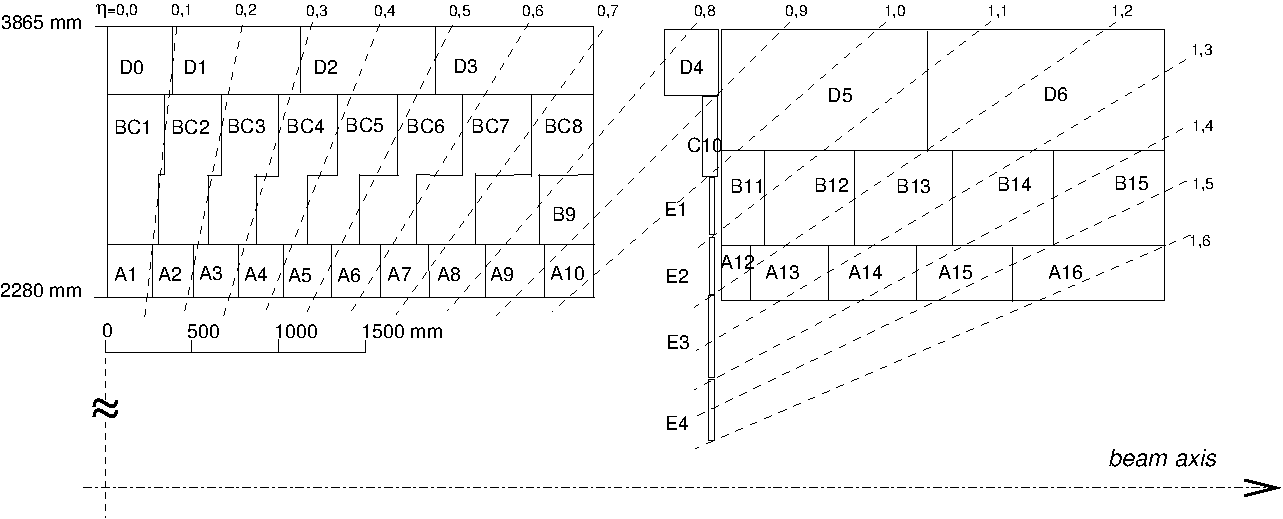
\includegraphics{figures/experiment/ATLAS_TILE_cell_layout}}
	}
	\caption{Schematic views of the ATLAS tile calorimeter, showing an individual module and the grouping of modules into readout cells.}
	\label{fig:ATLAS-calorimeters-tile}
\end{figure}



\subsubsection{Hadronic End-Cap Calorimeters}\label{sec:ATLAS-calorimeters-HEC}
Outside the tile calorimeter, two hadronic end-cap calorimeters (HEC) perform hadronic calorimetry in the pseudorapidity range $1.5<|\eta|<3.2$. The HECs use copper and LAr arranged into a flat plate geometry, as shown in figure~\ref{fig:ATLAS-calorimeters-HEC-layout}. Each HEC consists of two wheels (HEC1 and HEC2), which are further divided into two longitudinal segments.  The plates have an inner radius of $\SI{372}{\milli\meter}$ or $\SI{475}{\milli\meter}$ depending on $z$, and an outer radius of $\SI{2030}{\milli\meter}$. HEC1 contains 24 copper plates, each $\SI{24}{\milli\meter}$ thick and spaced by $\SI{8.5}{\milli\meter}$, plus a $\SI{12.5}{\milli\meter}$-thick front plate. HEC2 contains 16 copper plates measuring $\SI{50}{\milli\meter}$ in thickness, with a $\SI{25}{\milli\meter}$-thick front plate. The sampling fractions are thus $4.4\%$ for HEC1 and $2.2\%$ for HEC2. 

The gaps contain 3 electrodes spaced by $\SI{1.8}{\milli\meter}$, the outer two of which supply a nominal operating voltage of $\SI{1800}{\volt}$, and the middle of which performs the readout. The readout pads provide a transverse segmentation of $\Delta\eta\times\Delta\phi=0.1\times0.1$ for $|\eta|<2.5$, and $\Delta\eta\times\Delta\phi=0.2\times0.2$ for $2.5<|\eta|<3.2$. In total, 5,632 channels are read from the HEC. 

\begin{figure}[htbp]
	\centering
	\resizebox{0.6\textwidth}{!}{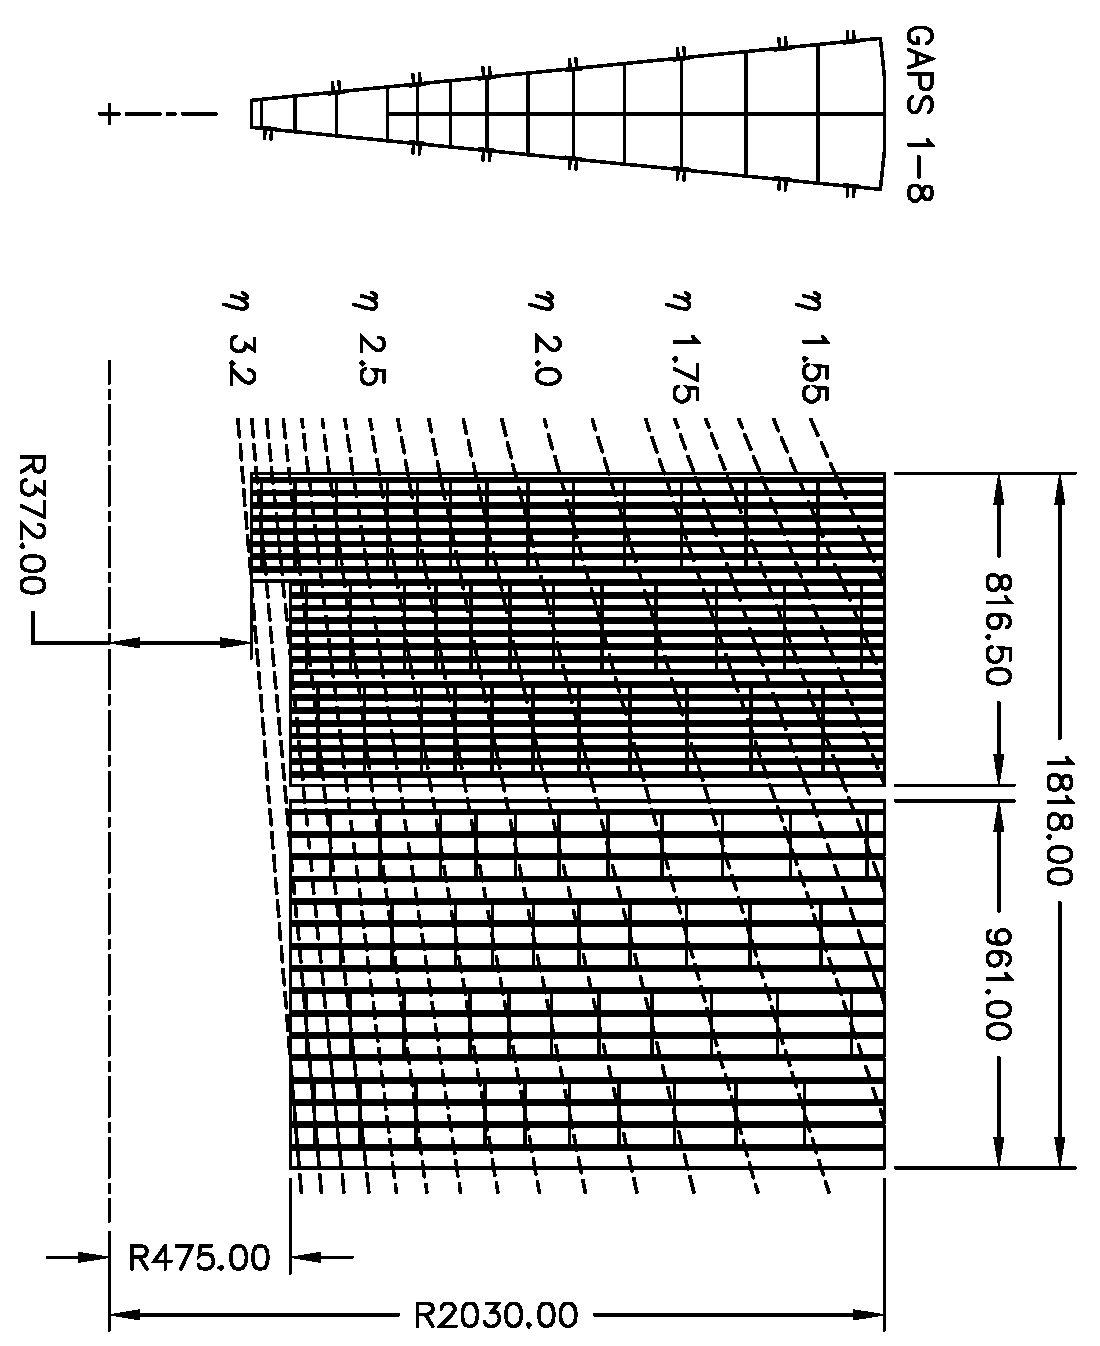
\includegraphics[angle=270]{figures/experiment/ATLAS_HEC_layout}}
	\caption{Schematic $R-\phi$ (left) and $R-z$ (right) views of the ATLAS hadronic end-cap calorimeters.}
	\label{fig:ATLAS-calorimeters-HEC-layout}
\end{figure}


\subsubsection{Forward Calorimeter}\label{sec:ATLAS-calorimeters-fcal}
The forward calorimeter (FCal) performs both electromagnetic and hadronic calorimetry in the very forward region, $3.2<|\eta|<4.9$, and also shields the muon system from high particle fluxes. On each side, the FCal is divided into three layers measuring $\SI{45}{\centi\meter}$ in depth, an electromagnetic layer (FCal1) and two hadronic layers (FCal2 and FCal 3). All three layers use LAr as the active medium, with very thin gaps due to avoid ion buildup due to the high particle flux. FCal1 uses copper absorbers to optimize the resolution and heat removal. FCal2 and FCal3 use tungsten absorbers, which provides good containment and reduces the lateral spread of hadronic showers. Finally, a passive brass plug behind FCal3 provides shielding for the muon system. The layout of the three layers and shielding plug is shown in figure~\ref{fig:ATLAS-calorimeters-fcal-layout}. 

FCal1 consists of stacked copper plates with $\SI{0.27}{\milli\meter}$ LAr gaps. The electrodes occupy 12,260 holes drilled through the copper plates, and consist of a copper rod coaxial with a copper tube, as shown in figure~\ref{fig:ATLAS-calorimeters-fcal1-electrodes}. FCal2 and FCal3 consist of two $\SI{2.35}{\centi\meter}$-thick copper end-plates spanned by an array electrodes similar to those in FCal1, except with tungsten rods, as shown in figure~\ref{fig:ATLAS-calorimeter-fcal23-electrodes}. The arrays contains 10,200 and 8,224 electrodes in FCal2 and FCal3, respectively. In total, the three layers, FCal1, FCal2, and FCal3, contain 1008, 500, and 254 readout channels, respectively, and constitute 27.6, 91.3, and 89.2 radiation lengths and 2.66, 3.68, and 60 interaction lengths. 

\begin{figure}
	\centering
	\resizebox{0.6\textwidth}{!}{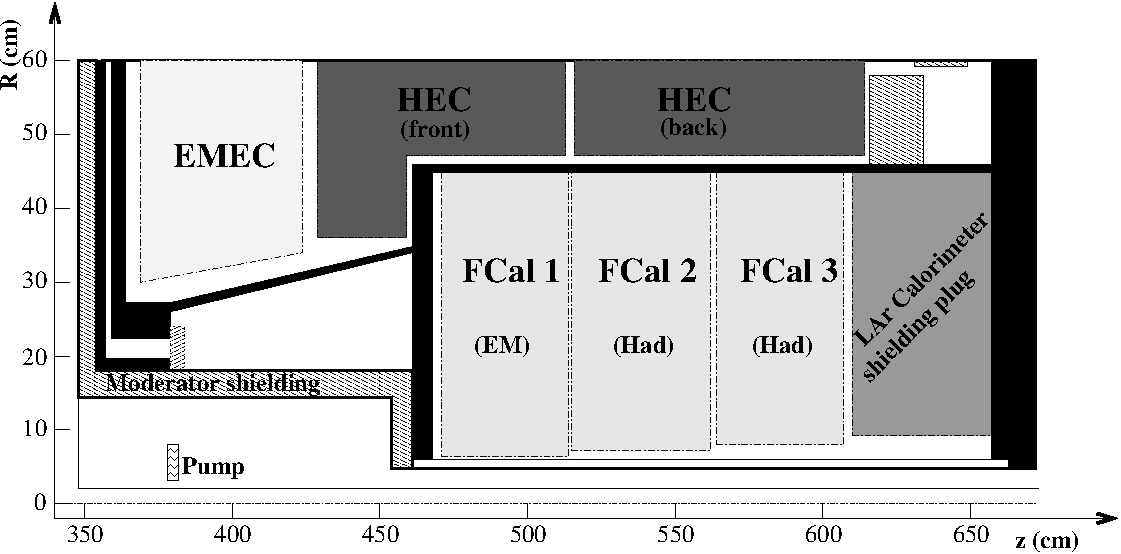
\includegraphics{figures/experiment/ATLAS_FCal_layout}}
	\caption{Schematic diagram showing the layout of the forward calorimeter in the $R$-$z$ plane.}
	\label{fig:ATLAS-calorimeters-fcal-layout}
\end{figure}


\begin{figure}
	\centering
	\subfloat[] {\label{fig:ATLAS-calorimeter-fcal1-electrodes}
		\resizebox{0.45\textwidth}{!}{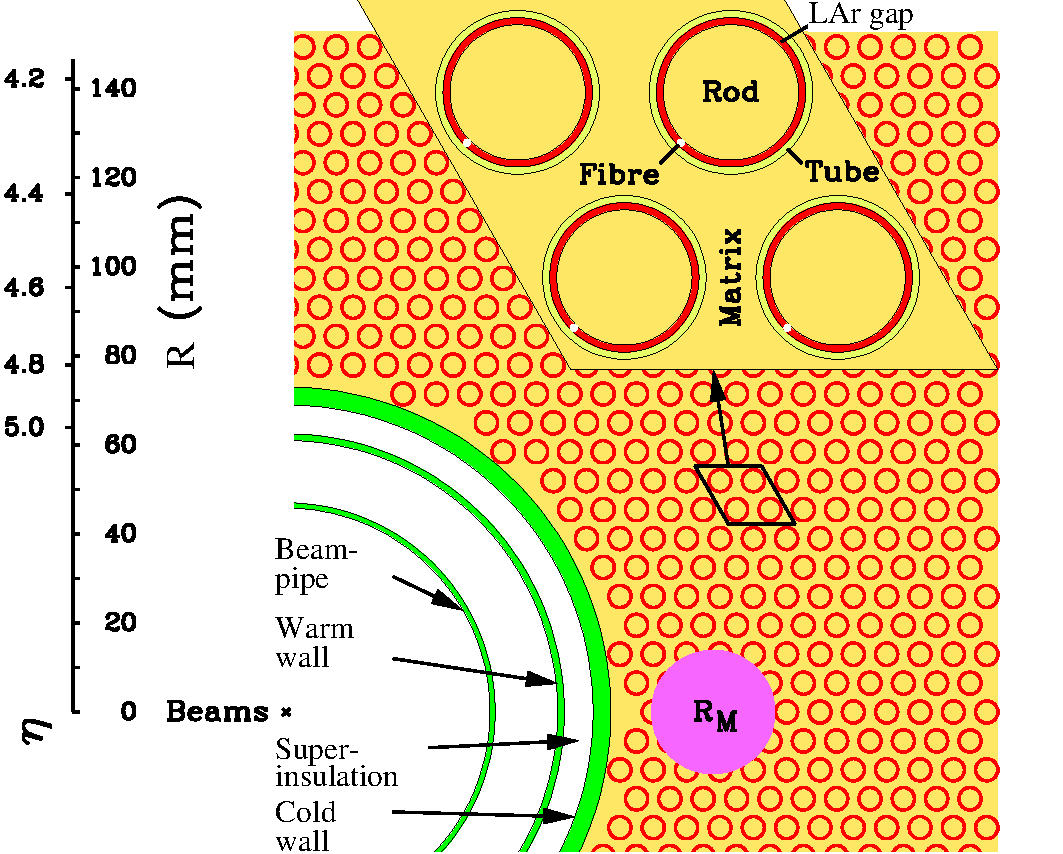
\includegraphics{figures/experiment/ATLAS_FCal1_electrodes}}
	}
	\subfloat[] {\label{fig:ATLAS-calorimeter-fcal23-electrodes}
		\resizebox{0.45\textwidth}{!}{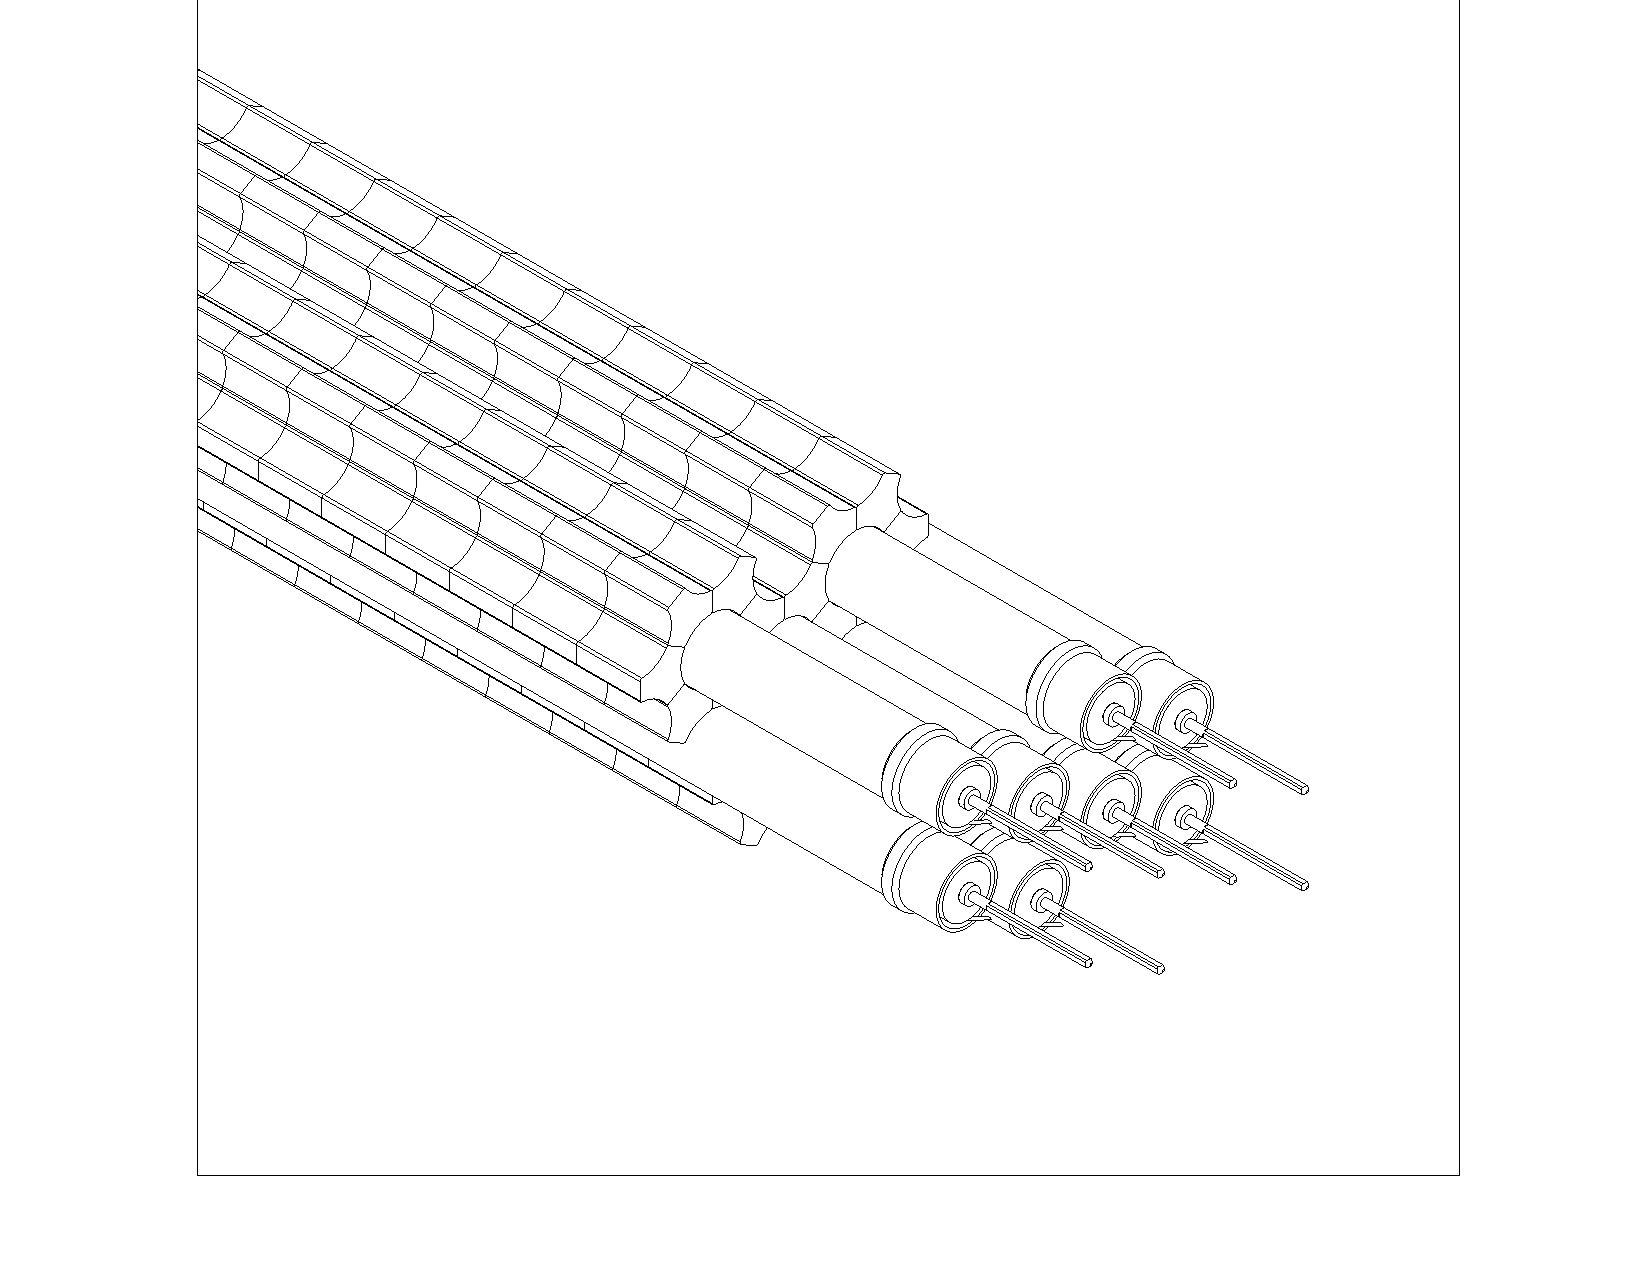
\includegraphics{figures/experiment/ATLAS_FCal23_electrodes}}
	}
	\caption{Left: the electrode structure of FCal1, showing the matrix of copper tubes and rods. The Moli{\`'e}re radius, $R_{\mathrm{M}}$, is shown for reference. Right: the absorber matrix in FCal2 and FCal, made from tungsten rods and copper tubes.}
	\label{fig:ATLAS-calorimeter-fcal-electrodes}
\end{figure}


\subsection{Muon Spectrometer}\label{sec:ATLAS-muon-spectrometer}
The muon spectrometer detects charged particles that penetrate the barrel and end-cap calorimeters. It forms the exterior of the ATLAS detector, occupying the volume of the barrel toroid with four large wheels on each side of the interaction point. Using a combination of several technologies, the muon spectrometer performs precision measurements of muon momenta in the region $|\eta|<2.7$, with a design resolution of 10\% for $\SI{1}{\tera\electronvolt}$ tracks, and also provides triggering on muons for $|\eta|<2.4$. 

The structure of the muon spectrometer is shown in figures~\ref{fig:ATLAS-muon-spectrometer-layout} and \ref{fig:ATLAS-muon-spectrometer-schematic}. The barrel systems are arranged in three layers with radii of approximately $\SI{5}{\meter}$, $\SI{7.5}{\meter}$, and $\SI{10}{\meter}$, mounted inside and on the eight coils of the barrel toroid magnet with approximate octagonal symmetry. The end-cap systems form four large wheels, located before and after the end-cap toroid magnets at positions of $|z|\approx \SI{7.4}{\meter},\ \SI{10.8}{\meter},\ \SI{14}{\meter},$ and $\SI{21.5}{\meter}$. 

\begin{figure}[htbp]
	\centering
	\resizebox{0.6\textwidth}{!}{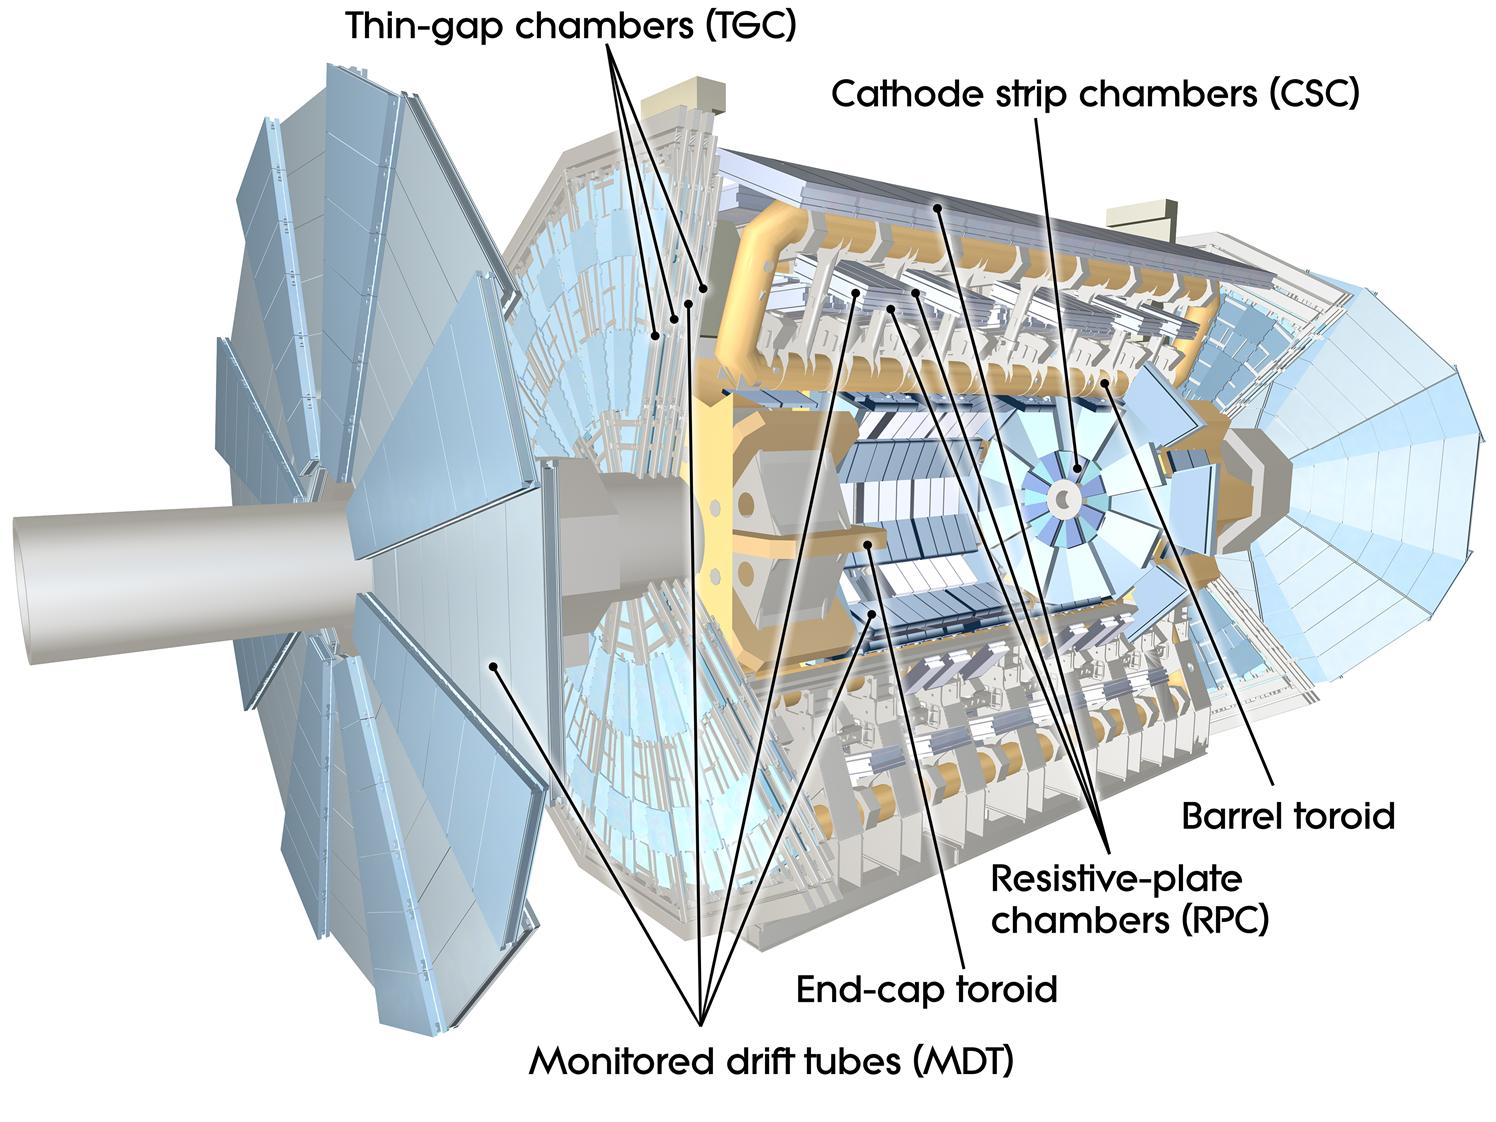
\includegraphics{figures/experiment/ATLAS_muons_sketch}}
	\caption{3D model of the ATLAS muon spectrometer. The four different types of detector (MDTs, CSCs, RPCs, and TGCs) and the toroid magnets are shown.}
	\label{fig:ATLAS-muon-spectrometer-layout}
\end{figure}

\begin{figure}[htbp]
	\centering
	\subfloat[ $R$-$z$ view of the muon spectrometer barrel. The barrel contains three layers, each with eight large and eight small chambers.] {
		\resizebox{0.4\textwidth}{!}{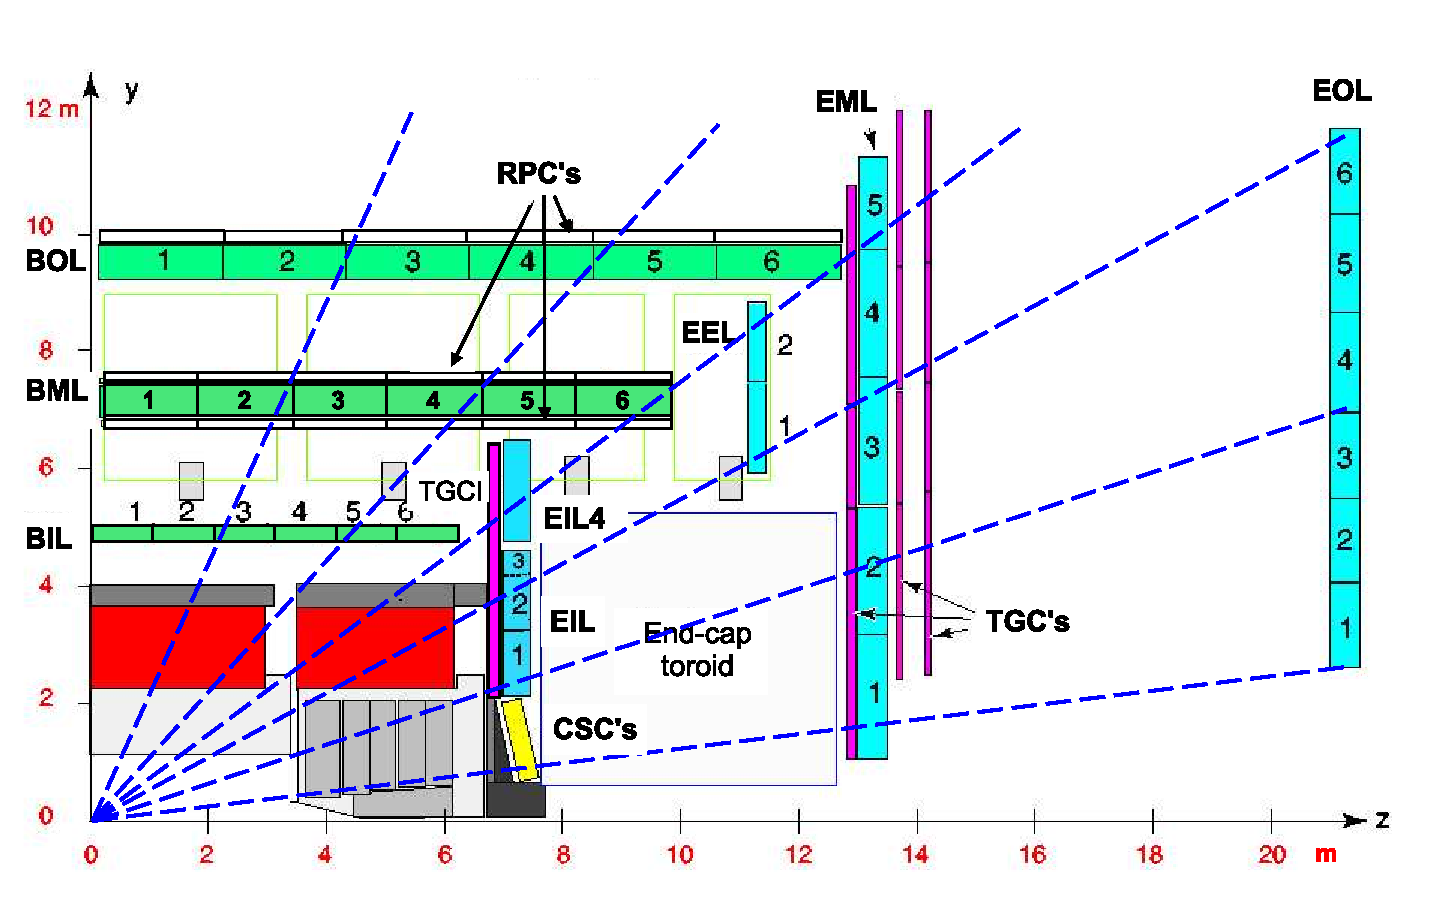
\includegraphics{figures/experiment/ATLAS_MS_layout_rz}}
	}
	\subfloat[ $R$-$\phi$ view of the muon spectrometer. The MDTs are shown in green and cyan, the CSCs in yellow, the TGCs in magenta, and the RPCs in white.] {
		\resizebox{0.4\textwidth}{!}{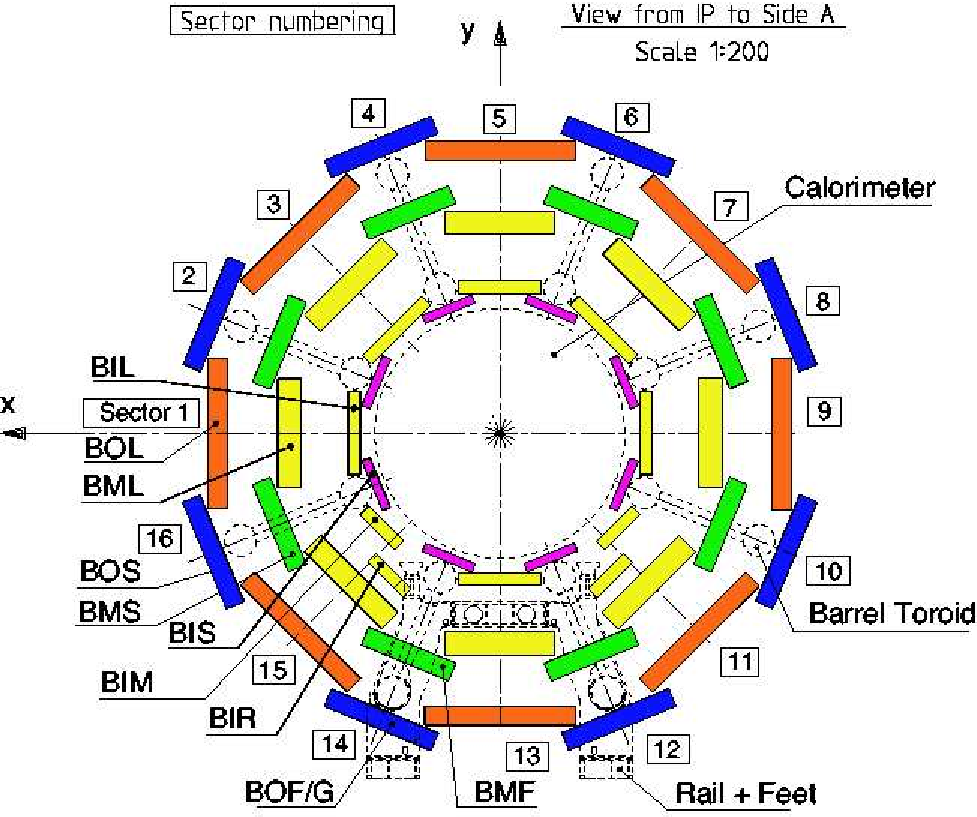
\includegraphics{figures/experiment/ATLAS_MS_layout_rphi}}
	}
	\caption{Layout of the chambers of the muon spectrometer.}
	\label{fig:ATLAS-muon-spectrometer-schematic}
\end{figure}



Four different technologies are used for precision measurements and triggering, depending on the location in the detector. Monitored drift tubes (MDTs) perform the precision measurements over most of the volume with $|\eta|<2.7$. Cathode strip chambers (CSCs) replace the MDTs in the innermost wheel for $2.0<|\eta|<2.7$, to handle the high particle flux. Triggering is performed by resistive plate chambers (RPCs) in the barrel ($|\eta|<1.05$) and thin gap chambers (TGCs) in the end-caps. The trigger chambers also supplement the MDT position measurements with the hit coordinate in the non-bending plane. 

\subsubsection{Monitored Drift Tubes}
The muon spectrometer contains 1088 MDT chambers, covering a total area of $\sim$\SI{550}{\meter\tothe{2}}. The majority of the MDT chambers are rectangular in the barrel and trapezoidal in the end-caps, and are laid out to optimize the solid angle coverage under the constraints of the magnet coils and other structures in the vicinity of the toroid magnet. Each chamber contains several drift tubes, as shown in figure~\ref{fig:ATLAS-MS-MDT-chamber}: the innermost chambers are divided into two groups of tube layers, called \emph{multilayers}, each with four layers of tubes, while the remaining chambers have two groups of three layers of tubes. 

\begin{figure}[htbp]
	\centering
	\resizebox{0.6\textwidth}{!}{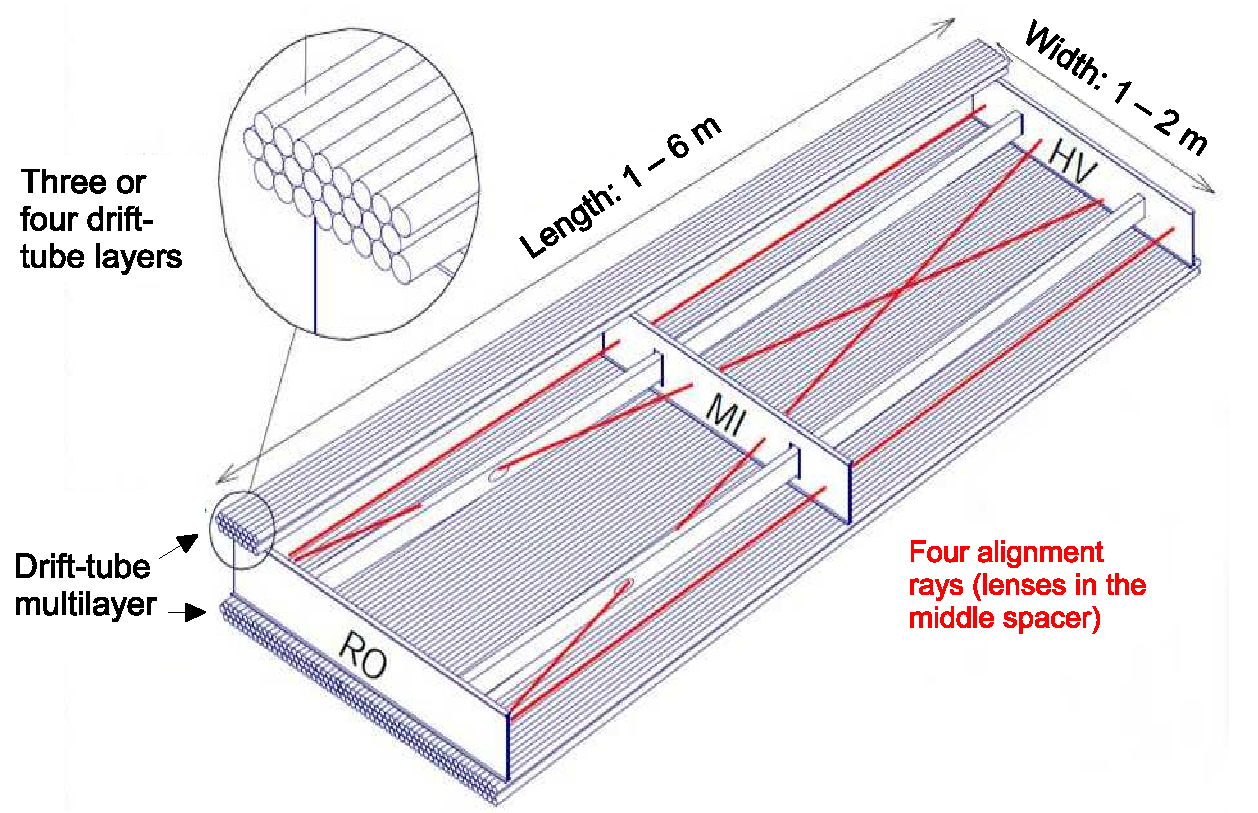
\includegraphics{figures/experiment/ATLAS_MDT_chamber}}
	\caption{The mechanical structure of a MDT chamber. Two multilayers, each consisting of three or four rows of drift tubes, are separated by aluminum spaceers. Four optical alignment rays continuously monitor the geometry of the chamber.}
	\label{fig:ATLAS-MS-MDT-chamber}
\end{figure}


The aluminum drift tubes have a radius of $\SI{29.97}{\milli\meter}$, with a $\SI{50}{\micro\meter}$-diameter tungsten-rhenium wire forming the anode along the axis of the tube. A cross section of a tube is shown in figure~\ref{fig:ATLAS-MS-MDT-xsec}. The operating voltage is $\SI{3080}{\volt}$, creating a radial electric field which allows for determination of the track position independent of the angle between the track and the tube. The tubes are filled with a mixture of argon and CO$_2$ (93:7) with a high pressure of 3~bar to reduce the impact of diffusion on the resolution. The gas mixture has good aging properties, but suffers from a long drift time, up to $\SI{700}{\nano\second}$ from the wall to the wire, and exhibits a nonlinear space-drift time relation which degrades the spatial resolution at high counting rates due to positive ions distorting the electric field. 

\begin{figure}
	\centering
	\resizebox{0.4\textwidth}{!}{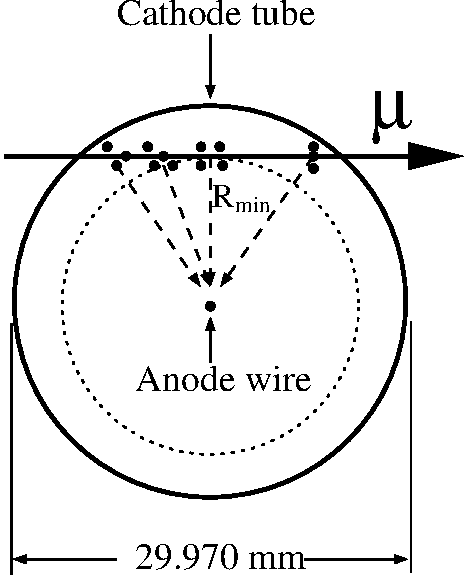
\includegraphics{figures/experiment/ATLAS_MDT_tube_cross_section}}
	\caption{Cross section of a drift tube, showing the cathode tube, the anode wire, and an illustration of a muon ionizing the gas as it traverses the tube.}
	\label{fig:ATLAS-MS-MDT-xsec}
\end{figure}

The average resolution of the drift tubes is $\SI{80}{\micro\meter}$, and the combined resolution of a chamber is $\SI{35}{\micro\meter}$. To achieve this precision, the position of the drift tubes and wires must be known to less than $\SI{30}{\micro\meter}$. Four optical alignment rays inside each MDT chamber continuously monitor the geometry of the chamber with a precision of a few microns, shown in figure~\ref{ATLAS-MS-MDT-chamber}. An inter-chamber optical alignment network monitors the relative positions of chambers relative to their neighbors with a precision of approximately $\SI{20}{\micro\meter}$. The optical alignment is supplemented with track-based alignment algorithms to align the chambers with poor or absent connection to the optical network, the end-caps with respect to the barrel, and the muon spectrometer with respect to the inner detector.




\subsubsection{Cathode Strip Chambers}
The rate limit for the safe operation of the MDTs is about \SI[per-mode=fraction]{150}{\hertz\per\centi\meter\tothe{2}}, which is exceeded for $|\eta|>2$ in the first layer of the end-cap at $|z|\approx 7~\mbox{m}$. Accordingly, CSCs are used in this volume of the detector, which can operate up to rates of about 1~kHz/\cm$^2$. Eight large and eight small trapezoidal chambers give full coverage in $\phi$, as shown in figure~\ref{fig:ATLAS-MS-CSC-layout}.  

The CSCs are multiwire proportional chambers, with parallel wires running in the radial direction and the two cathodes finely segmented in perpendicular directions to provide measurements in both the $\eta$ and $\phi$ directions. The perpendicular cathode segmentation provides position measurements in two dimension, aiding the resolution of nearby hits from more than one track. In the bending direction, the segmentation corresponds to a readout pitch of $5.31~\mm$ and $5.56~\mm$ for the large and small chambers, respectively.  The track coordinate is determined from a relative measurement of the charge induced on 3-5 adjacent strips at the peak of the charge distribution, shown schematically in figure~\ref{fig:ATLAS-MS-CSC-charge}. The resolution, dominated by electronic noise in the pre-amplifiers and by the spread of charge along the anode wire due inclined tracks, delta electrons, or a Lorentz force along the wire, is roughly $60~\micron$ per CSC plane. In the non-bending direction, a coarser segmentation leads to a resolution of $5~\mm$. 

\begin{figure}[htbp]
	\centering
	\subfloat[] {\label{fig:ATLAS-MS-CSC-layout}
		\resizebox{0.4\textwidth}{!}{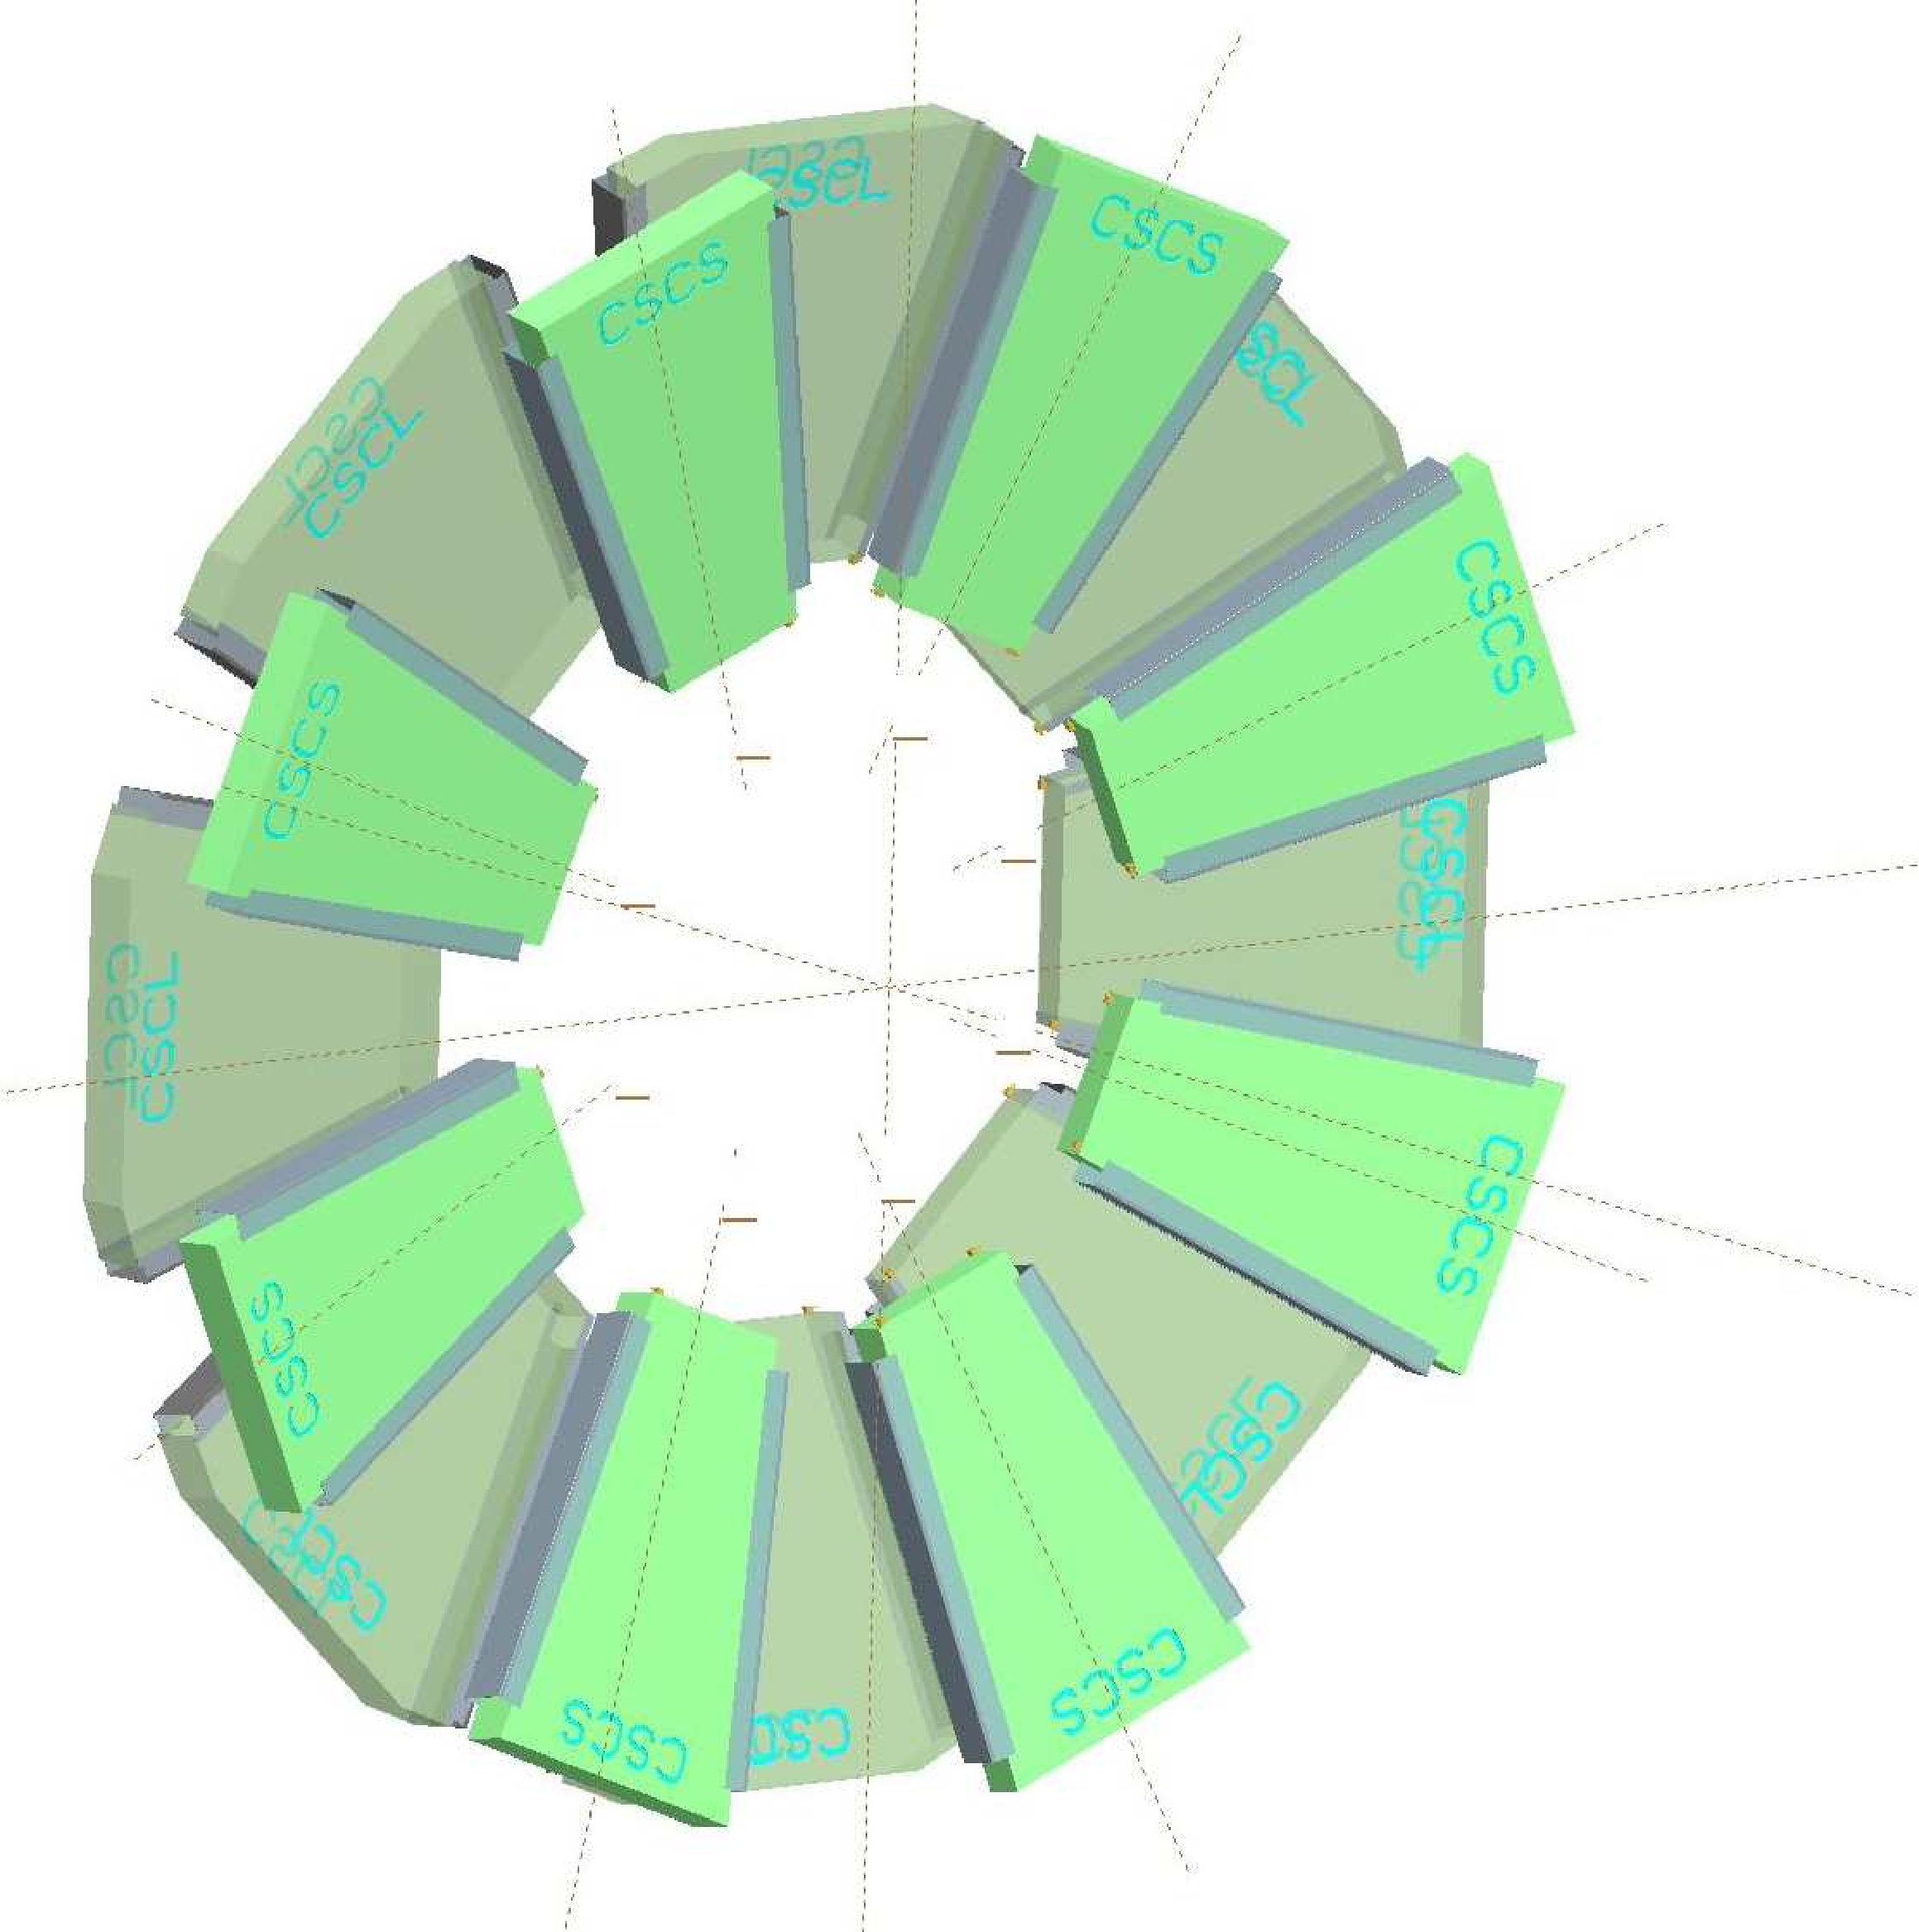
\includegraphics{figures/experiment/ATLAS_CSC_geometry}}
	}
	\subfloat[] {\label{fig:ATLAS-MS-CSC-segmentation}
		\resizebox{0.4\textwidth}{!}{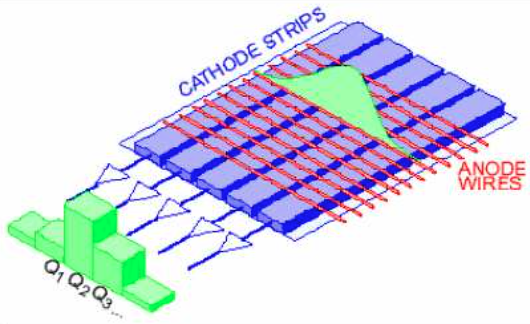
\includegraphics{figures/experiment/ATLAS_CSC_readout_strips2}}
	}
	\caption{Left: Layout of the eight large and eight small CSC chambers. Right: Schematic view of the CSC anode wires and perpendicular cathode strips, showing the deposition of charge from a track on several adjacent strips.}
	\label{fig:ATLAS-MS-CSC}
\end{figure}


\subsubsection{Resistive Plate Chambers}
Muon triggering in the barrel ($|\eta|<1.05$) is performed by 544 RPCs, which exhibit good spatial and timing resolution and an adequate rate capability of $\sim1~\mbox{kHz}/\cm^2$. The RPCs form three layers, or \emph{stations}, with two on either side of the middle MDT layer and the third on the inner or outer side of the outer MDT layer, for the small and large sectors, respectively. Each station has two independent layers, each providing a measurement of $\eta$ and $\phi$, resulting in six possible measurements for muons passing through three stations. 

An RPC unit consists of two sets of two parallel resistive plates ($2~\mm$-thick phenolic-melaminic plastic laminate) separated by $2~\mm$ by insulating spacers, shown in figure~\ref{fig:ATLAS-MS-RPC-schematic}. The interior is filled with a gas mixture of C$_2$H$_2$F$_4$/Iso-C$_4$H$_{10}$/SF$_6$ (94.7/5/0.3). With an electric field of $4.9~\mbox{kV}/\mm$, muons traversing the gas induce an avalanche towards the anode, which is read out via capacitive coupling to $25$-$35~\mm$-wide copper strips on the exterior face of the RPC. The RPCs achieve a spatial resolution of approximately $10~\mm$ in $z$ and $\phi$, a timing resolution of $1.5~\ns$, and a detection efficiency of $\sim 98\%$. 

\begin{figure}[htbp]
	\centering
	\resizebox{0.6\textwidth}{!}{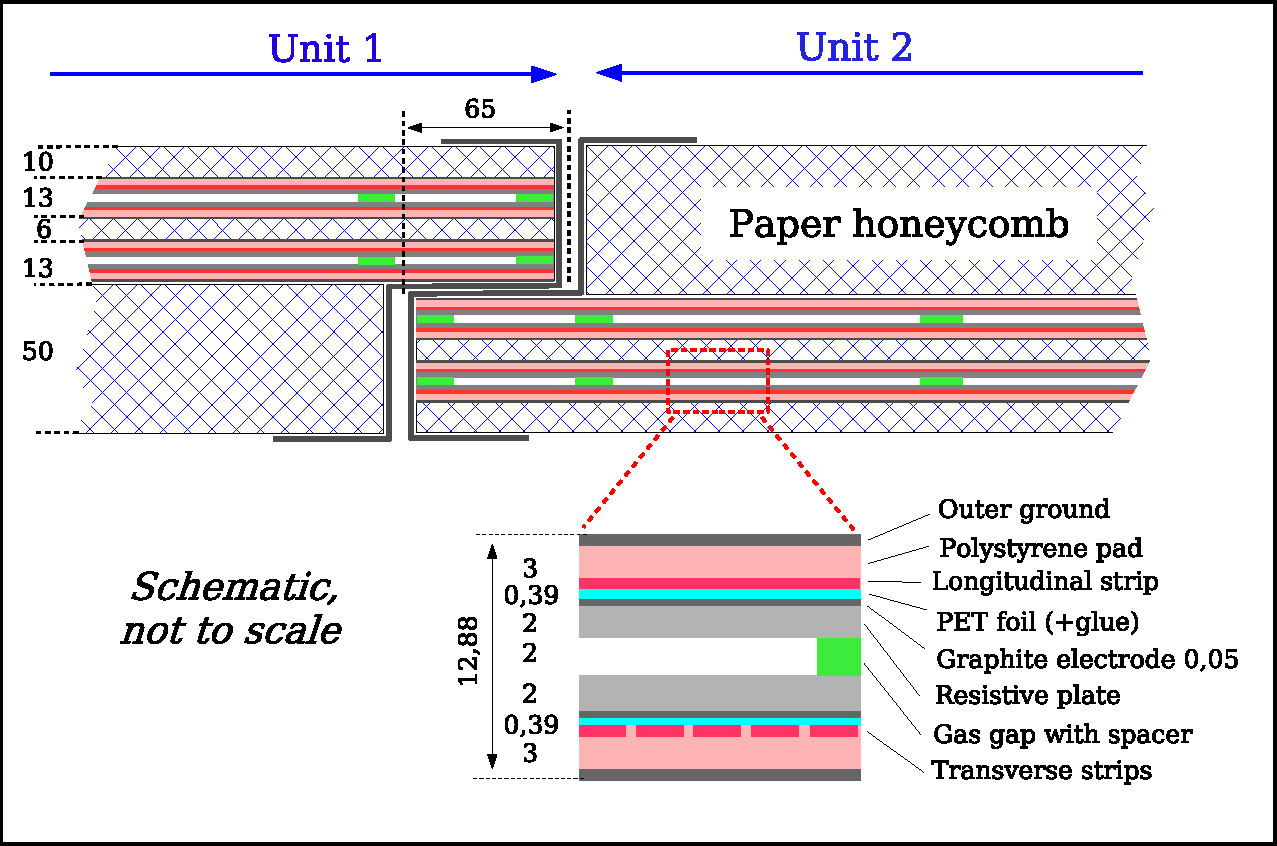
\includegraphics{figures/experiment/ATLAS_RPC_structure}}
	\caption{Cross section of an RPC, showing two units joined to form a single chamber. Each unit has two sets of two resistive plates (grey) separated by insulating spacers (green). The readout strips (magenta) are on the opposite side of the resistive plates from the gas gap. Outside the detecting elements, the volume of the RPC chamber is filled with paper honeycomb. The dimensions are given in millimeters.}
	\label{fig:ATLAS-MS-RPC-schematic}.
\end{figure}

\subsubsection{Thin Gap Chambers}
TGCs provide muon triggering in the end-caps, due to their good timing resolution and high rate capability. The TGCs also provide an azimuthal coordinate measurement, which complements the MDT measurement in the radial direction. Nine TGC disks are installed in total: a doublet mounted near the inner MDT end-cap layer, and a triplet and two doublets near the middle MDT end-cap layer. The disks are divided into two concentric annuli, one covering $1.05\leq |\eta| \leq 1.92$ and the other covering $1.92\leq|\eta|\leq2.4$. 

\begin{figure}[htbp]
	\centering
	\subfloat[ Cross sectional views of a TGC trilepton and a TGC doublet. The dimensions of the gas gaps are enlarged to show their structure.] {\label{fig:ATLAS-MS-TGC-triplet-doublet}
		\resizebox{0.5\textwidth}{!}{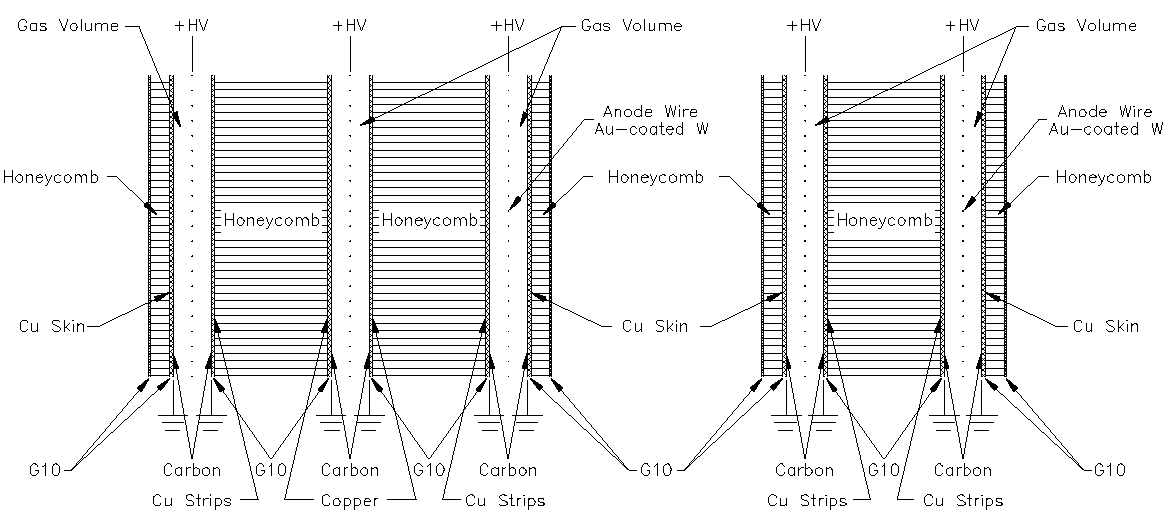
\includegraphics{figures/experiment/ATLAS_TGC_construction}}
	}
	\hfill
	\subfloat[ Closeup view of the TGC structure, showing the anode wires, graphite cathodes, and copper readout strips..] {\label{fig:ATLAS-MS-TGC-structure}
		\resizebox{0.4\textwidth}{!}{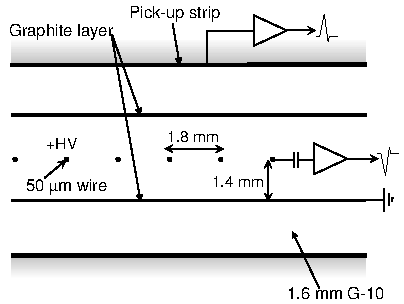
\includegraphics{figures/experiment/ATLAS_TGC_structure}}
	}
	\caption{The construction of the TGCs.}
	\label{fig:ATLAS-MS-TGC}
\end{figure}

The TGCs are multiwire proportional chambers filled with a gas mixture of CO$_2$ and $n$-pentane. The cathode planes are $1.6~\mm$-thick FR4 (Flame Resistant 4) plates, with the interior faces coated with graphite and exterior faces cladded with copper. The triplet TGCs have three layers of wires and two layers of copper readout strips, while the doublet TGCs have two layers each of wires and strips, as shown in figure~\ref{fig:ATLAS-MS-TGC-triplet-doublet}. The radial coordinate is measured by the anode wire groups and the azimuthal coordinate by the radial cathode strips. The chambers are ``thin'' in that the wire to cathode distance, $1.4~\mm$, is shorter than the wire-to-wire distance of $1.8~\mm$, as shown in figure~\ref{fig:ATLAS-MS-TGC-structure}. The anode wires have a diameter of $50~\micron$ and are operated at a potential of $2.9~\mbox{kV}$. The small wire-to-wire distance and high electric field near the anode wires contribute to a good timing resolution of $4~\ns$. The spatial resolution, $2$-$6~\mm$ in $R$ and $3$-$7~\mm$ in $\phi$, is determined by the ganging of readouts: due to the direction of the magnetic field, achieving the required momentum resolution at fixed transverse momentum requires finer resolution at larger pseudorapidities. 


\subsection{Trigger and Data Acquisition}
During a typical data-taking run during 2012, the LHC beam contains 1377 bunches with a typical bunch spacing of $50 \us$, giving an event rate of $\sim 20~\mbox{MHz}$. In contrast, the ATLAS data acquisition system records events at roughly $400~\mbox{Hz}$. The filtering of events is performed by the three-level ATLAS triggering system. The first level, L1, is implemented in hardware, and reduces the event rate to less than $75~\mbox{kHz}$. The second level, L2, is implemented in software, and reduces the event rate to less than $3.5~\mbox{kHz}$ using regions of interest (RoIs) identified by the L1 trigger. The final level of the trigger, the Event Filter, is also implemented in software, and reduce the event rate to less than $400~\mbox{Hz}$ using the full event information. 

The L1 trigger reduces the event rate from $20~\mbox{MHz}$ to $75~\mbox{kHz}$ using a limited subset of the event data. While the L1 trigger is processing an event, the full event data is stored in buffers on the detector. Due to the limited buffer size, the L1 latency must be less than $2.5 \us$, of which $1 \us$ is used by the cable propagation time. Therefore, the trigger is implemented in custom hardware processors. The block diagram for the trigger is shown in figure~\ref{fig:ATLAS-trigger-L1-block}. The inputs to the trigger include the RPC and TGC detectors in the muon spectrometer and all of the calorimeter system.  Two primary systems, the L1 Calorimeter Trigger and the L1 Muon Trigger, select events based on the presence of high-$\Et$ objects or significant total event activity. These include high-$\pt$ muons, electron and photons, jets, hadronically decaying tau leptons, large missing transverse energy, and large total transverse energy. 

The L1 Calorimeter Trigger uses about 7,000 analogue trigger towers with a reduced granularity, $\Delta\eta\times\Delta\phi=0.1\times0.1$ for most of the detector. Two subsystems run in parallel: the cluster processor identifies electrons/photons and hadronically decay tau lepton candidates with $\Et$ above a programmable set of thresholds, while the jet/energy-sum processor identifies jets and calculates the total scalar transverse energy and $\Etmiss$ using $\Delta\eta\times\Delta\phi=0.2\times0.2$ blocks of calorimeter cells. Isolation cuts can be applied as well, limiting the energy allowed in the towers surrounding the object of interest and, in the case of electrons/photons, in the hadronic towers behind the electromagnetic towers. 

The L1 Muon Trigger searches for a coincidence of hits in consecutive muon trigger stations within a \emph{road}, roughly corresponding to the path of a muon from the interaction point through the detector. The $\pt$ threshold is encoded in the width of the road, with a narrower road corresponding to a higher $\pt$ threshold. For low-$\pt$ muons in the RPCs, the algorithm begins with hits in the second RPC doublet, called the \emph{pivot plane}. The trigger requires a hit in the first RPC doublet, within the road defined by the interaction point and the hit in the pivot plane. The high-$\pt$ algorithm is similar, requiring a hit along the road in the third RPC doublet as well as the first two.In the end-caps, the pivot plane is established by the outermost layer of TGCs, with the road corresponding to the path of an infinite-momentum muon originating from the interaction point. To reject backgrounds from random coincidences, stricter requirements are imposed on the number of coincident hits in the TGC doublets and triplets.

The muon and calorimeter triggers pass their decisions along with the corresponding data to the Central Trigger Processor (CTP). The CTP communicates the total trigger decision to the front ends on the detector, including special triggers such as random triggers or the minimum bias trigger based on scintillator counters. In the event of a passed trigger, the event data is passed to the L2 trigger. The CTP also manages the \emph{luminosity blocks}, an index representing the time at which an event was recorded with coarse ($\sim1$ minutes) granularity. A luminosity block is the shortest time interval for which the integrated luminosity can be determined such that the total uncertainty is dominated by systematic effects, rather than limited statistics. In the event of a detector failure, this index allows the rejection of a minimal set of affected events. 

The L2 trigger reduces the event rate from a maximum of $75~\mbox{kHz}$ from the L1 trigger to less than $3.5~\mbox{kHz}$. The trigger is implemented in software, and uses only the subset of the event data within the RoIs identified by the L1 trigger, typially $1$-$2\%$ of the total. After a successful L1 trigger, the data corresponding to the RoIs, stored in the detector-specific front end electronics, are accumulated in the RoI builder via 1574 readout links. The RoI builder combines the 1574 event fragments into a single data structure, which is passed to the L2 processing farm. At each step of a given trigger algorithm targeting particular signatures, only the relevant RoIs are analyzed. If no signatures remain valid, the event is rejected. Hence the full RoI information is transferred only for events which pass the L2 selection criteria. The typical L2 latency is about $40 \ms$.

Finally, the event filter reduces the event rate to the final $\sim400~\mbox{Hz}$ read out from the detector to disk. Also implemented in software, it runs the same algorithms as used in the offline event reconstruction using the full event information. Based on the objects used for triggering, the triggered events are categorized into one or more \emph{data streams}. The data streams and other data computed by the event filter are appended to the event data, which are then transferred to CERN’s central data-recording facility for storage. An example of the event filter rates from the various streams during a single data-taking run is shown in figure~\ref{fig:ATLAS-trigger-EF-rates-singlerun}. The monthly average rates of each stream during 2012 are shown in figure~\ref{fig:ATLAS-trigger-EF-rates-2012}.

\begin{table}[htbp]
	\centering
	\subfloat[ Event filter rates for a single data-taking run.] {\label{fig:ATLAS-trigger-EF-rates-singlerun}
		\resizebox{0.4\textwidth}{!}{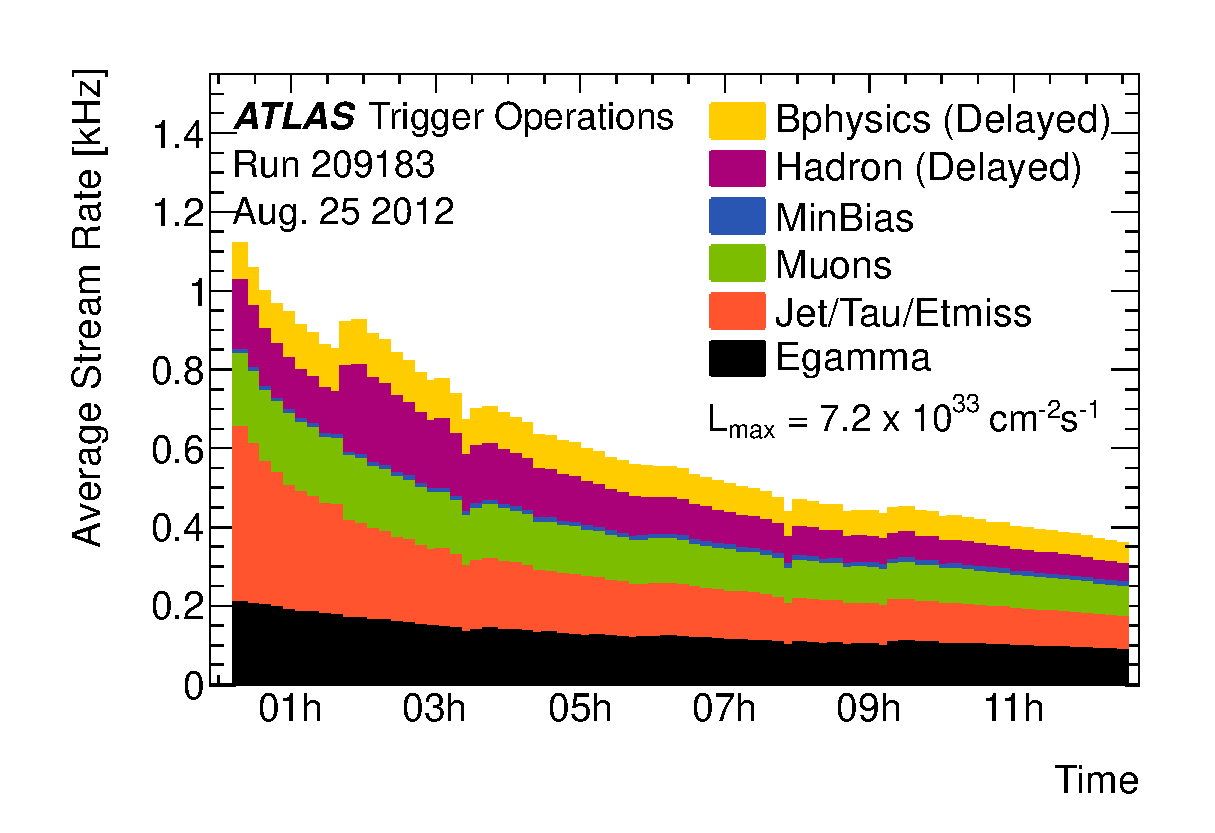
\includegraphics{figures/experiment/ATLAS_trigger_streamrates_singlerun.eps}}
	}
	\hfill
	\subfloat[ Average monthly event filter rates during 2012.] {\label{fig:ATLAS-trigger-EF-rates-2012}
		\resizebox{0.55\textwidth}{!}{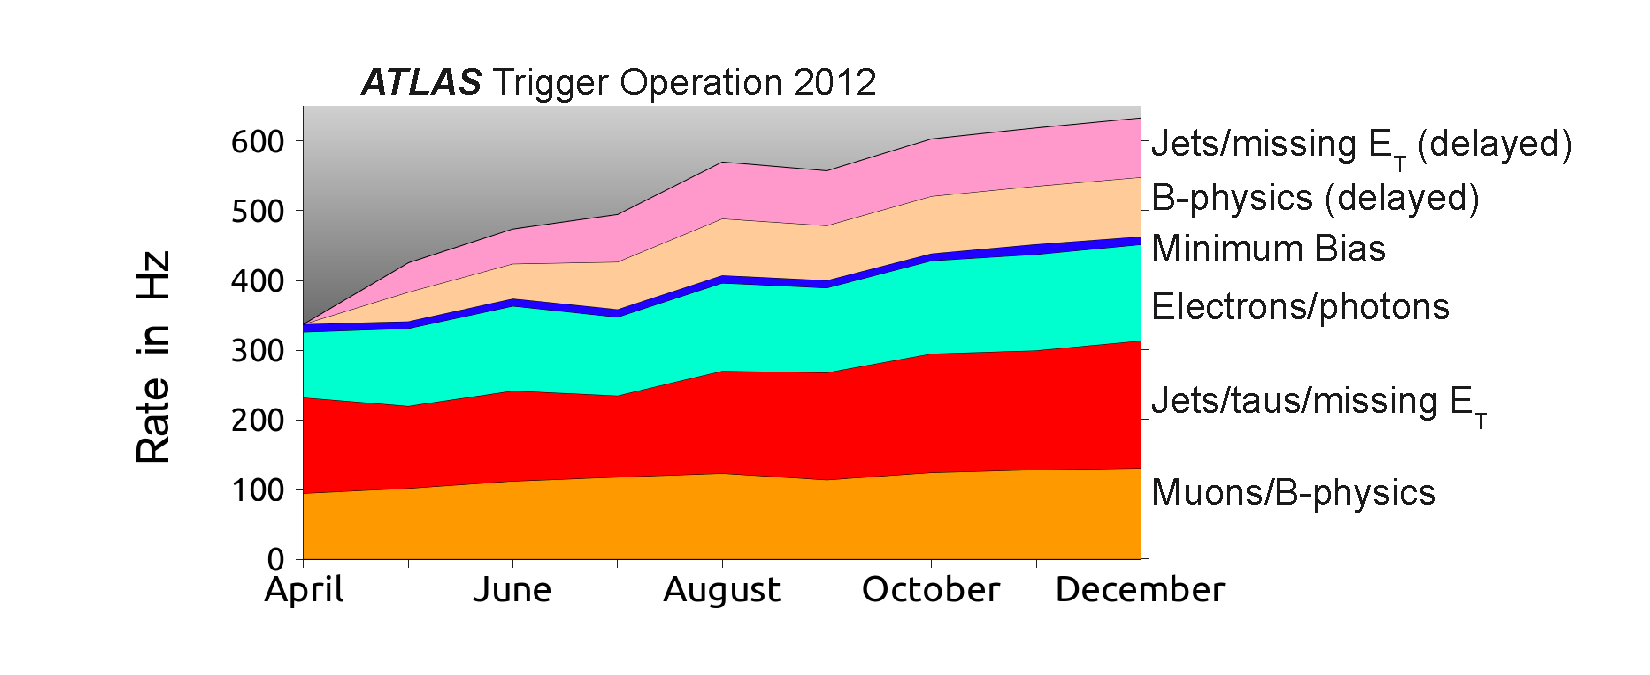
\includegraphics{figures/experiment/ATLAS_trigger_streamrates_2012}}
	}
	\caption{The rates of recording events from the event filter for different data streams.}
	\label{fig:ATLAS-trigger-EF-rates}
\end{table}


\printbibliography